%% GRB 081125496 — spectral and timing analysis (single-pulse campaign, burst #1)
%% DRAFT — all numbers real and provisional-flagged; produced by the staged
%% pipeline (AGENTS.md), one manuscript section per pipeline step.
\documentclass[twocolumn]{aastex631}

\newcommand{\grb}{GRB~081125496}
\newcommand{\pgstat}{\mathrm{PGstat}}

\shorttitle{\grb}
\shortauthors{Chand, Sharma, \& Joshi}

\begin{document}

\title{\grb}

\author{Agentic AI Report by Vikas Chand, Khushboo Sharma, and Jagdish C. Joshi}
\noaffiliation

\begin{abstract}
We present a complete timing and time-resolved spectral analysis of the bright
single-pulse burst \grb\ using \textit{Fermi}/GBM data, as the first burst of a
106-burst single-pulse campaign executed with a staged, gate-reviewed pipeline.
The windowed duration is $T_{90} = 8.50^{+0.15}_{-0.19}$~s with $5.3\sigma$ of
emission beyond the analysis window, the pulse is FRED-like (two-sigmoid
asymmetry $\varphi = 0.317 \pm 0.026$), and the per-band durations follow
$T_{90} \propto E^{-0.14 \pm 0.02}$. The minimum variability timescale depends
on the estimator by design: a windowed method finds $33.9 \pm 2.9$~ms on the
pulse rise, while global wavelet methods return $215 \pm 17$~ms (CWT) and
$546 \pm 69$~ms (Haar) for the same data. The spectral lag between 25--50 and
100--300~keV is $\tau = 0.705^{+0.291}_{-0.205}$~s (soft lagging hard), which
for a single broad pulse we interpret as envelope evolution: $\tau/T_{90}
\approx 0.08$. We then fit 24 spectral models in nine Bayesian-block time bins
and in the time-integrated spectrum, selecting by the Akaike Information
Criterion. A cutoff power law suffices in seven of nine resolved bins; a
high-energy tail is demanded only on the pulse rise and in the late tail, where
the Band function wins with $\beta \simeq -2.1$. The time-integrated winner, a
smoothly broken power law plus power law, wins no resolved bin: the integrated
``extra component'' is spectral evolution in disguise. Across $\sim$90
blackbody-added fits we find zero photospheric evidence; every low-$kT$
solution is an edge-constrained artifact at the fitted band's lower boundary.
We discuss the implications of estimator- and window-dependence for population
lag--variability correlations. All figures and numbers in this paper passed
independent verification gates; the analysis provenance is machine-auditable.
\end{abstract}

\keywords{Gamma-ray bursts (629) --- Time domain astronomy (2109)}

\section{Introduction} \label{sec:intro}

Single-pulse gamma-ray bursts offer the cleanest laboratory for prompt-emission
physics: one emission episode, no pulse overlap, and a light curve whose
spectral evolution can be followed from rise to decay without deconvolution.
They anchor pulse-paradigm descriptions of GRB variability
\citep{1996ApJ...459..393N,2003ApJ...596..389K}, spectral-lag physics
\citep{2010ApJ...711.1073U,2012MNRAS.419..614U}, curvature-effect tests
\citep{2013ApJ...778....3S}, and searches for spectral components beyond a
single continuum \citep{2019A&A...625A..60R,2019ApJ...886...20Y}.

\grb\ (\textit{Fermi}/GBM trigger bn081125496; $\mathrm{RA}=42\fdg7$,
$\mathrm{Dec}=-18\fdg9$) is a bright single-pulse burst with a GBM catalog
duration of $T_{90} = 9.28 \pm 0.61$~s and a 10--1000~keV fluence of
$1.85\times10^{-5}$~erg~cm$^{-2}$. It is burst \#1 of a 106-burst
single-pulse campaign whose sample is selected on light-curve morphology, not
brightness. This paper presents the complete per-burst analysis --- detector
selection through time-resolved spectroscopy and timing --- and doubles as the
reference implementation of the campaign's staged pipeline: each section below
corresponds to one pipeline step, and each step's products passed through
independent verification gates before entering this manuscript
(\S\ref{sec:provenance}).

\section{Observations and Data} \label{sec:data}

\grb\ triggered the \textit{Fermi} Gamma-ray Burst Monitor
\citep{2009ApJ...702..791M} on 2008 November 25. We use time-tagged event
(TTE) data from the NaI and BGO detectors. Following the convention of
\citet{2020ApJ...903....9C}, spectral fits use NaI channels in 8--900~keV with
the 30--40~keV iodine K-edge region excluded, and BGO channels in
0.2--38~MeV. Data in every band are retained subject to data-quality cuts
only; no detection-significance cut is applied, to avoid biasing the census of
spectral shapes.

\section{Detector Selection} \label{sec:detsel}

The campaign selects NaI detectors with source angles $\le 50\arcdeg$
(with a 50--60$\arcdeg$ rescue for detectors flagged in the burst catalog) and
the BGO on the source side. For \grb\ this yields NaI detectors $n_a$
(reference, smallest angle) and $n_b$, and BGO $b_1$
(Figure~\ref{fig:step1}). All subsequent analysis uses these three detectors.

\begin{figure}
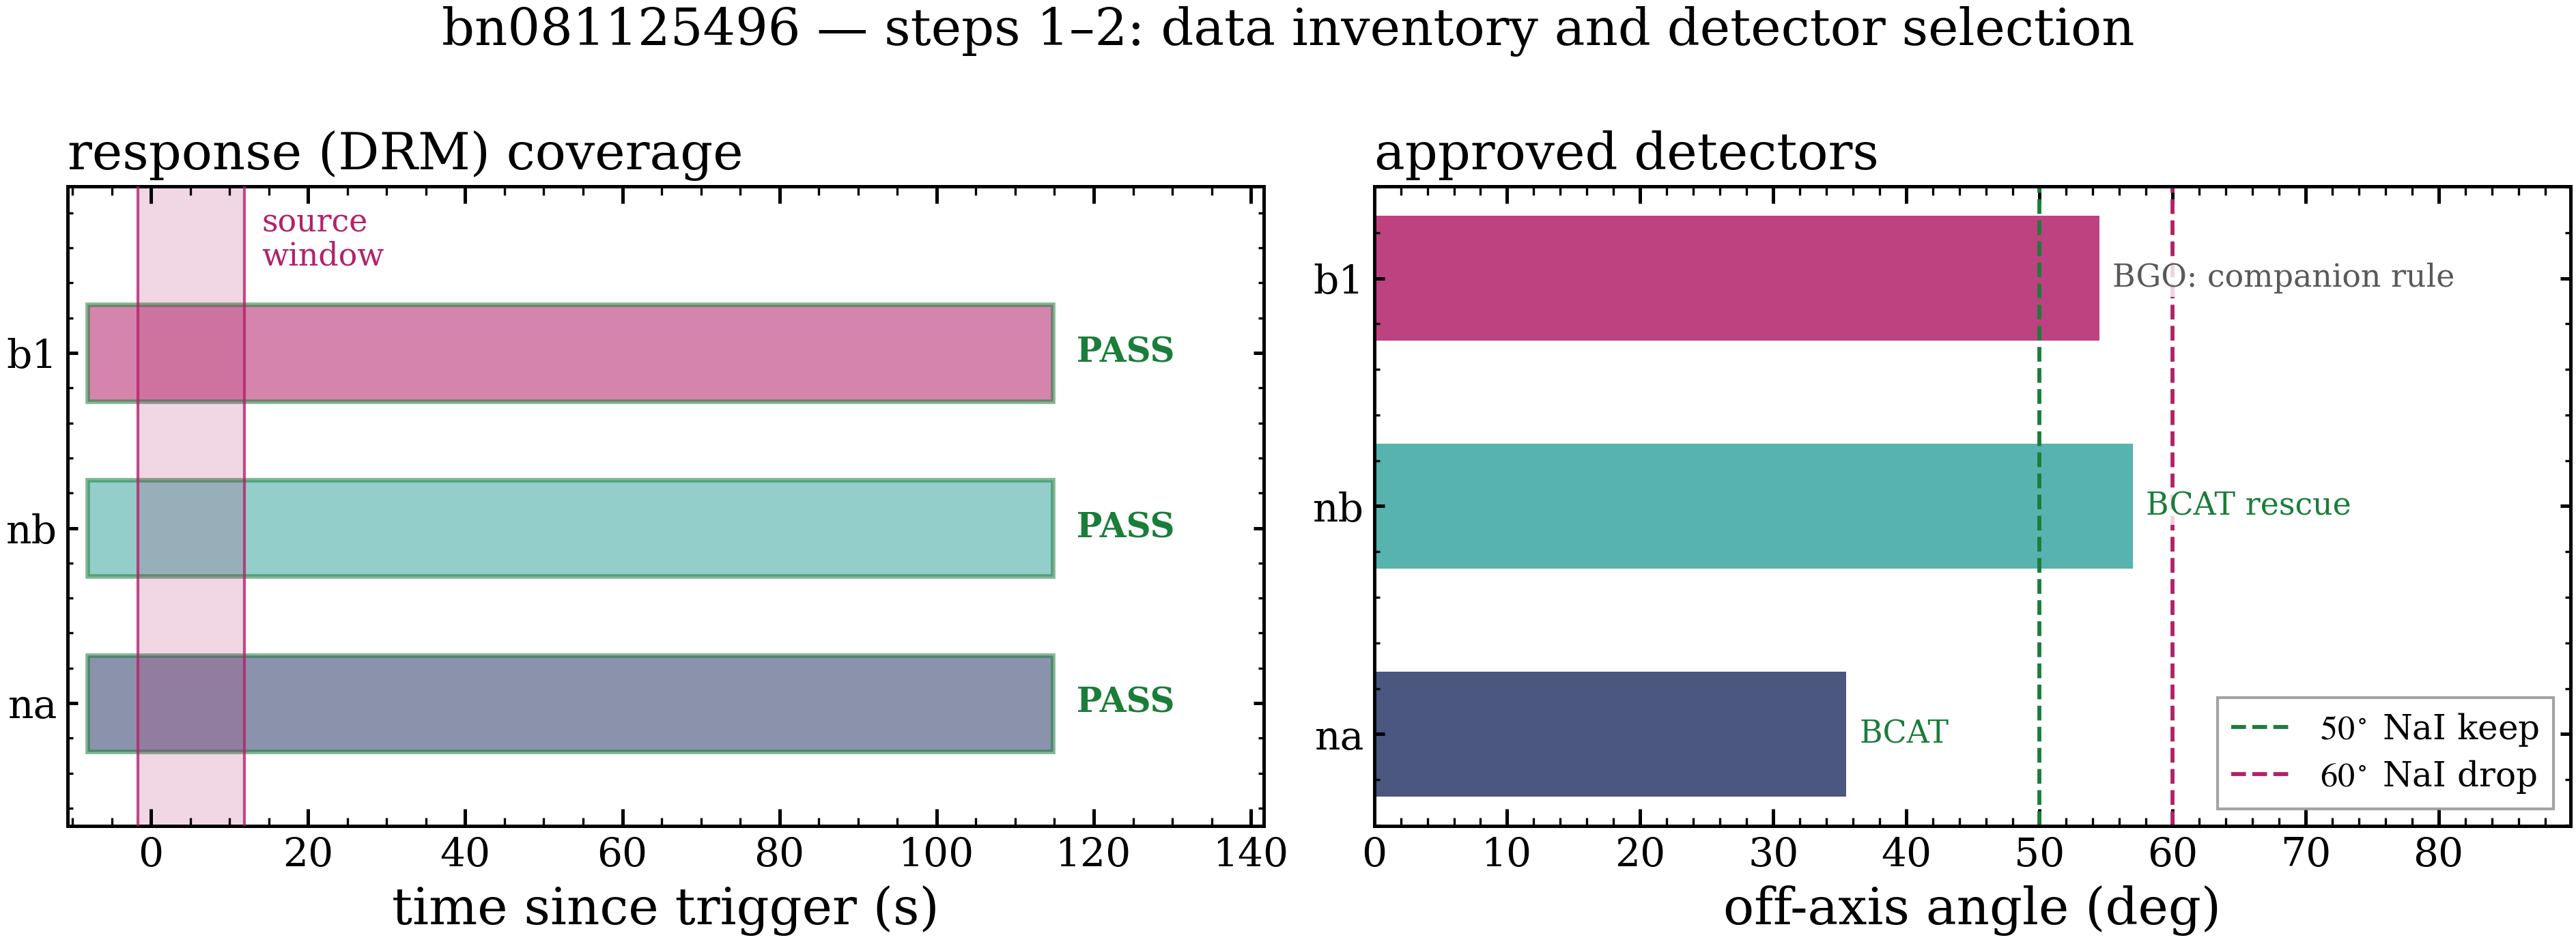
\includegraphics[width=\columnwidth]{figs/bn081125496_step1_inventory.png}
\caption{Detector selection for \grb: source angles for all GBM detectors with
the $50\arcdeg$ selection rule and the $50$--$60\arcdeg$ catalog-rescue band;
the selected detectors ($n_a$, $n_b$, $b_1$) and their data coverage.
\label{fig:step1}}
\end{figure}

\section{Background and Source Intervals} \label{sec:stage1}

Background and source intervals were selected interactively by a human
reviewer using a gtburst-style two-panel interface, and are recorded with
approval stamps in the campaign catalog. For \grb\ the background is fit on
per-detector pre- and post-burst windows ($n_a$: $(-23.5,-8.0)$ and
$(30,140)$~s; $n_b$: $(-21.0,-6.0)$ and $(17,75)$~s; $b_1$: $(-21.0,-6.0)$ and
$(21,81)$~s) with polynomial orders selected per detector (0--3), and the
approved source window is $(-1.7, 11.9)$~s (Figures~\ref{fig:step3}, \ref{fig:step4}). The background
windows deliberately hug the burst, and the same approved selections drive
both the spectroscopy and the timing analysis --- a single set of human
decisions propagates through every product.

\begin{figure}
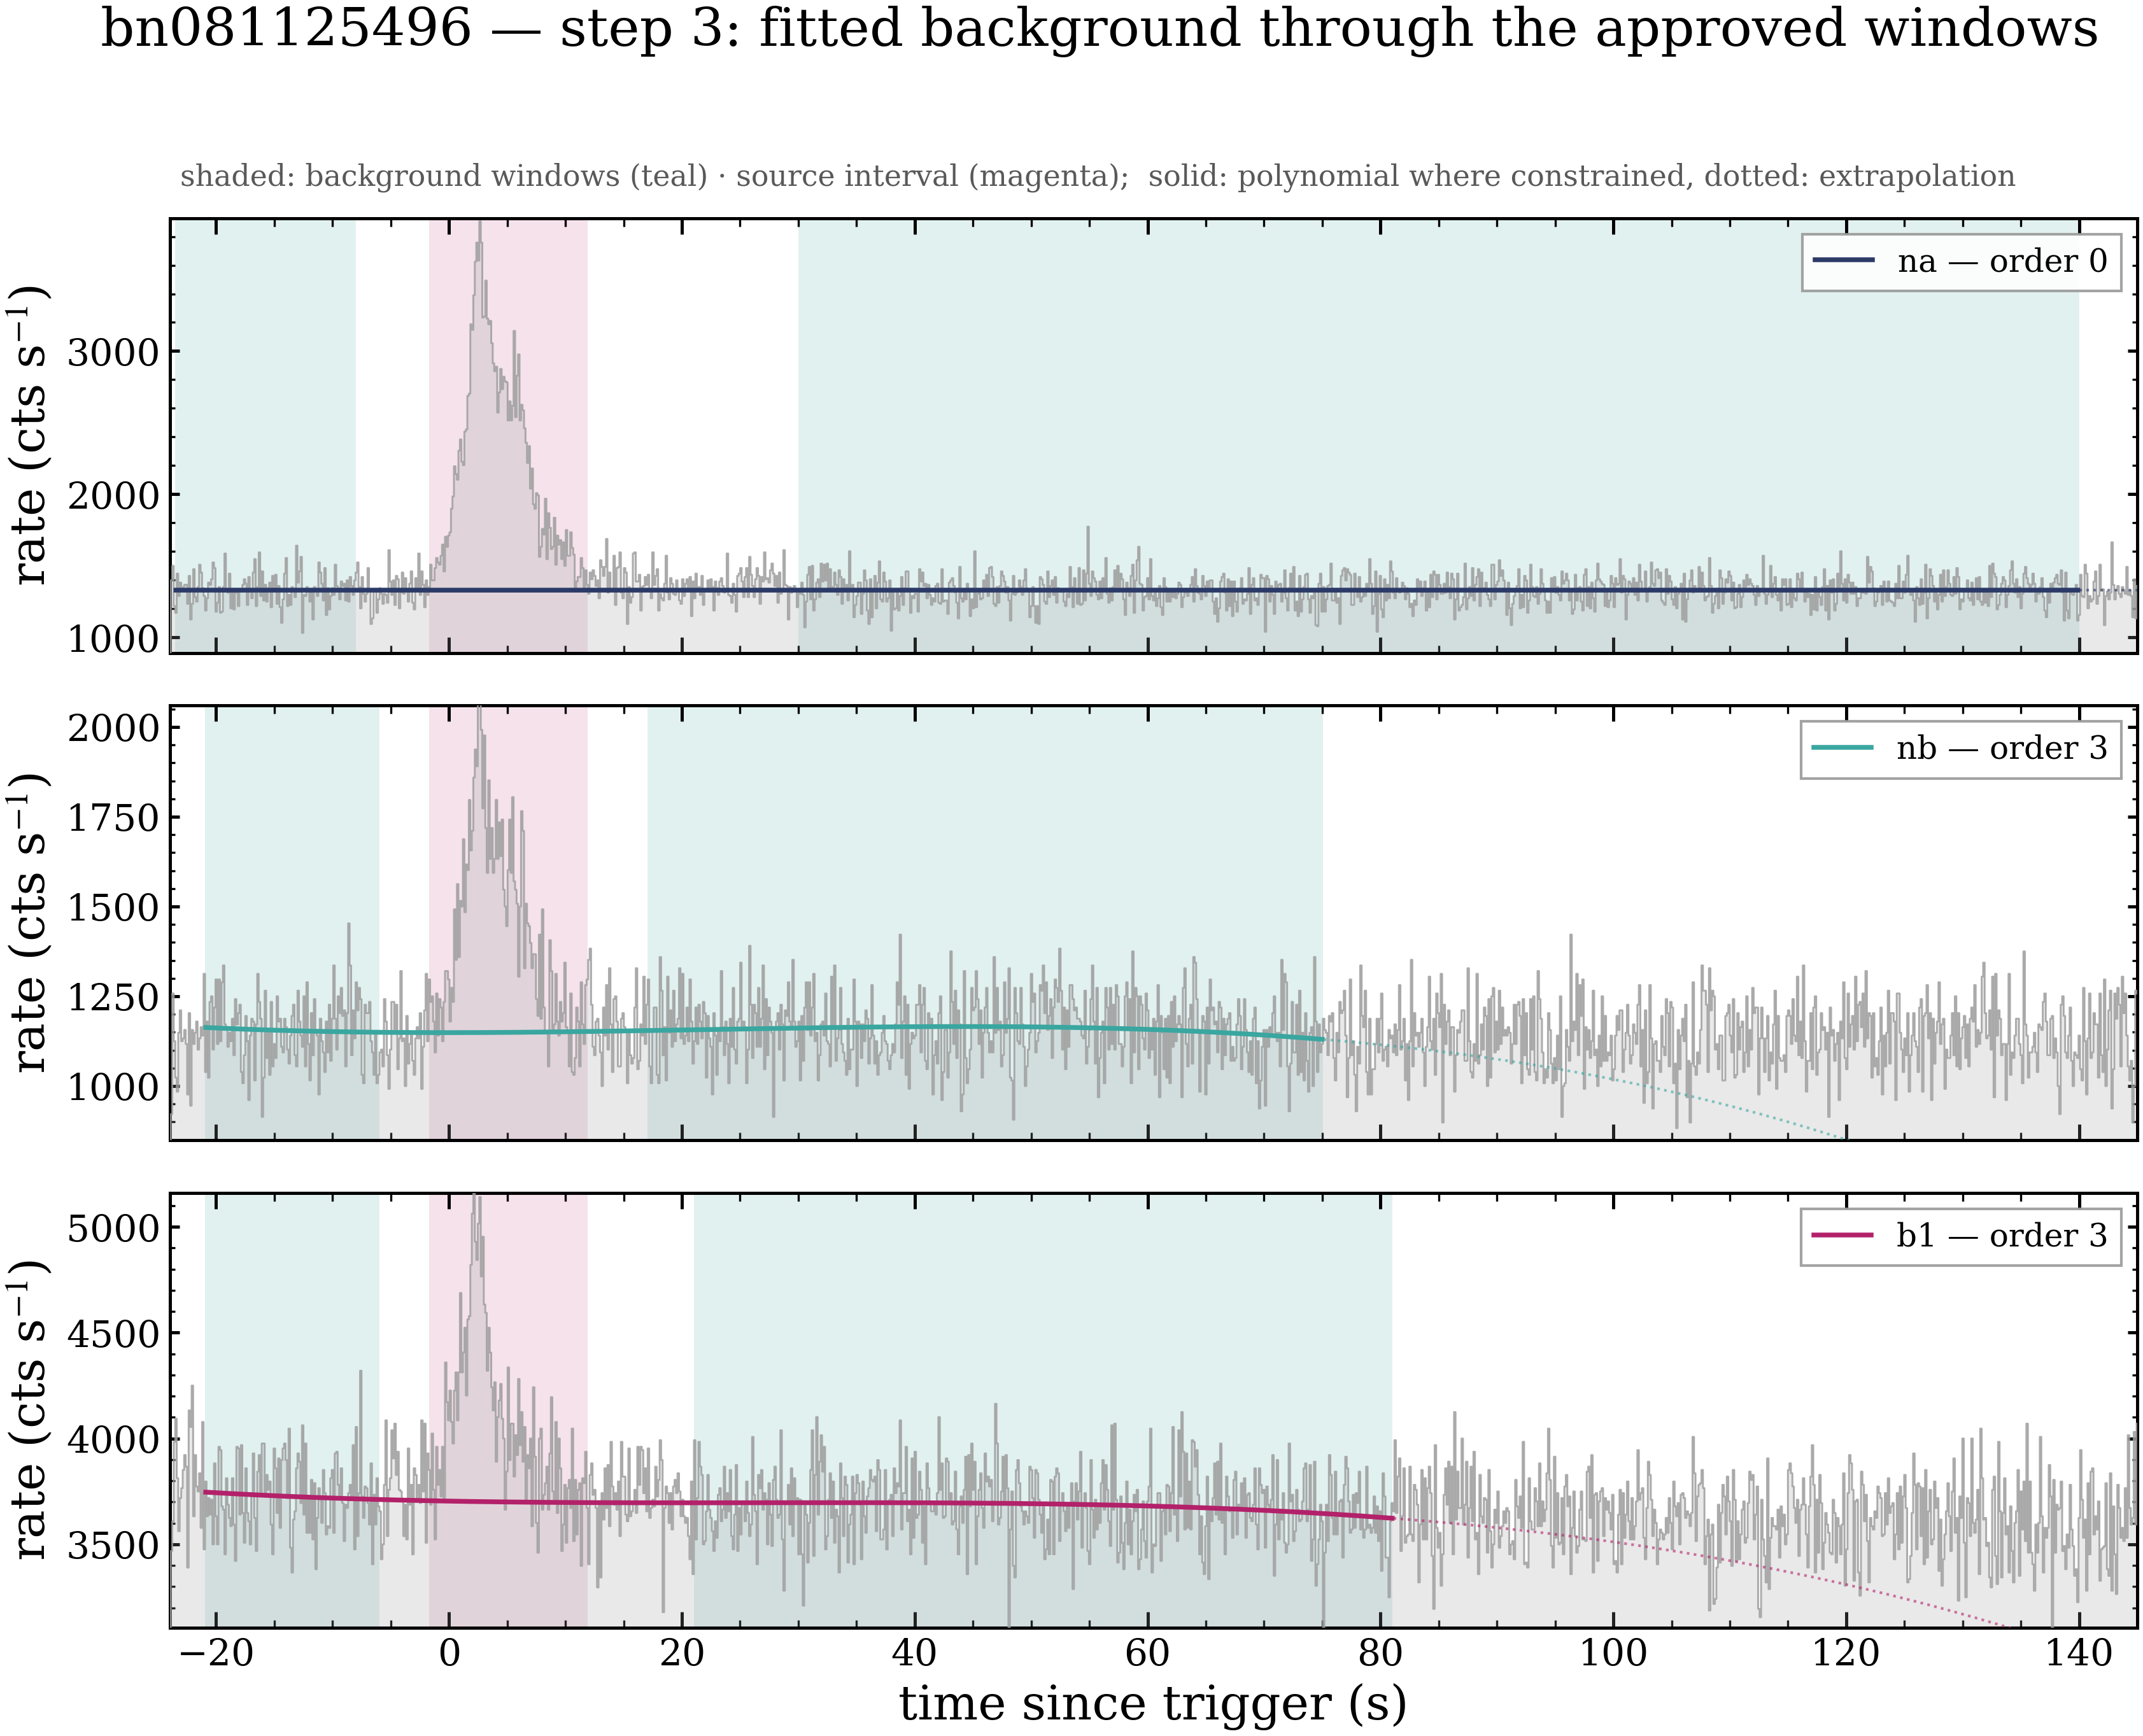
\includegraphics[width=\columnwidth]{figs/bn081125496_step3_background.png}
\caption{Approved background intervals and polynomial fits for the three
selected detectors. \label{fig:step3}}
\end{figure}

\begin{figure}
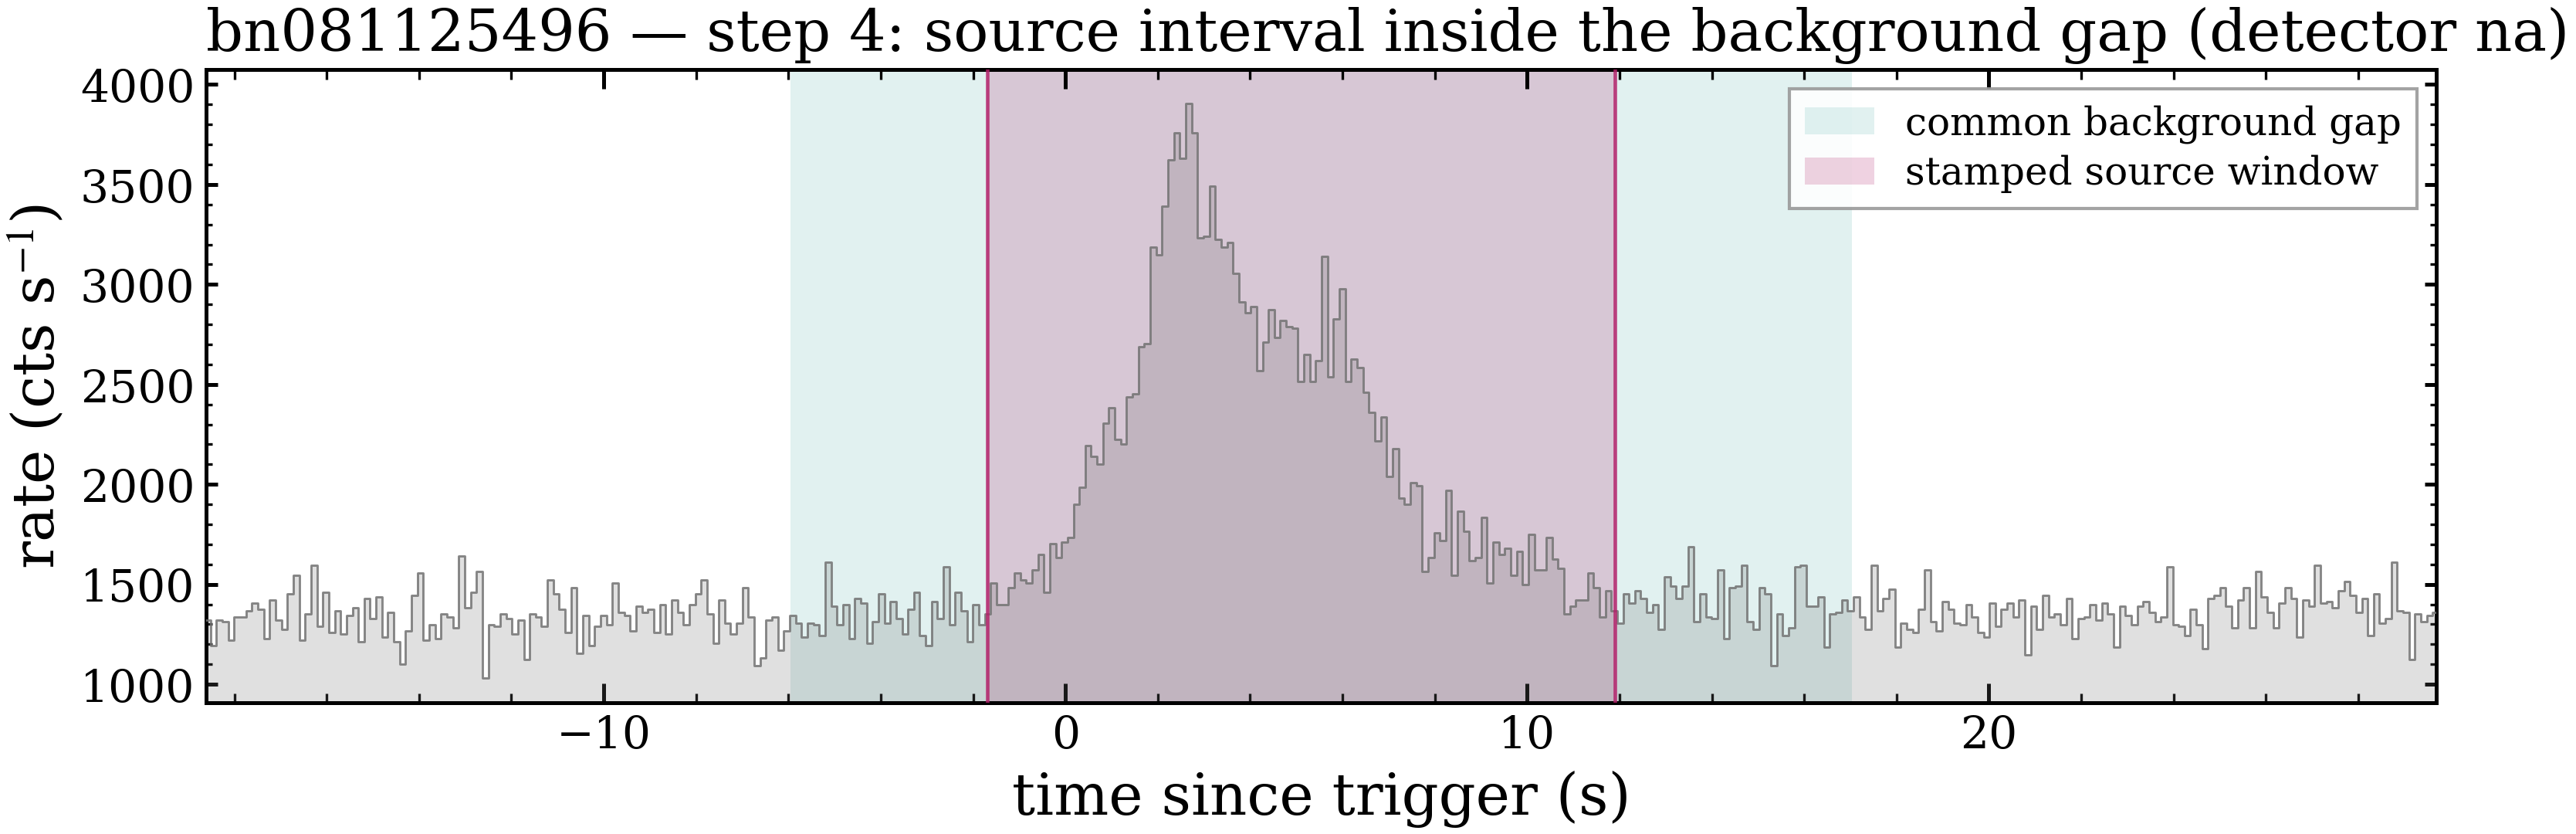
\includegraphics[width=\columnwidth]{figs/bn081125496_step4_source.png}
\caption{Approved source interval over the background-subtracted light curve.
\label{fig:step4}}
\end{figure}

\section{Timing Analysis} \label{sec:timing}

All timing measurements run on the approved selections of \S\ref{sec:stage1},
on the reference NaI; the spectroscopy (\S\ref{sec:spectra}) uses the same
selections.

\subsection{Durations} \label{sec:durations}

We measure durations inside the approved source window with a
first-crossing cumulative estimator; uncertainties come from Poisson
realizations of the raw counts propagated through the identical estimator,
with the $t_5$--$t_{95}$ covariance retained
\citep[cf. the quadrature approximation of][]{2013ApJ...763...15Q}. We find
$T_{90} = 8.50^{+0.15}_{-0.19}$~s spanning $[0.47, 8.97]$~s and
$T_{50} = 3.50$~s. Emission continues beyond the window: the interval between
the source window and the post-burst background window holds
$5.3\sigma$ ($\approx 790$ net counts) of excess, so our $T_{90}$ is a
\emph{windowed lower limit}, consistent with the catalog
$9.28 \pm 0.61$~s \citep{2017ApJ...844..126S} once the excluded tail and the
count-space/fluence-space methodological difference are accounted for.
The same truncation applies to the spectroscopy: all spectral statements
describe the windowed emission.

Per-band durations decrease with energy from $9.4 \pm 0.2$~s (8--25~keV) to
$6.6 \pm 0.3$~s (100--350~keV), following
$T_{90} \propto E^{-0.14 \pm 0.02}$ ($\chi^2/\mathrm{dof} = 0.5$;
Figure~\ref{fig:step7}), consistent within $2\sigma$ with the
population-mean slope $-0.20 \pm 0.02$ of \citet{2013ApJ...763...15Q} ---
which we treat as a consistency check, not a per-burst law
\citep[cf.][]{1993ApJ...413L.101K}.

\begin{figure*}
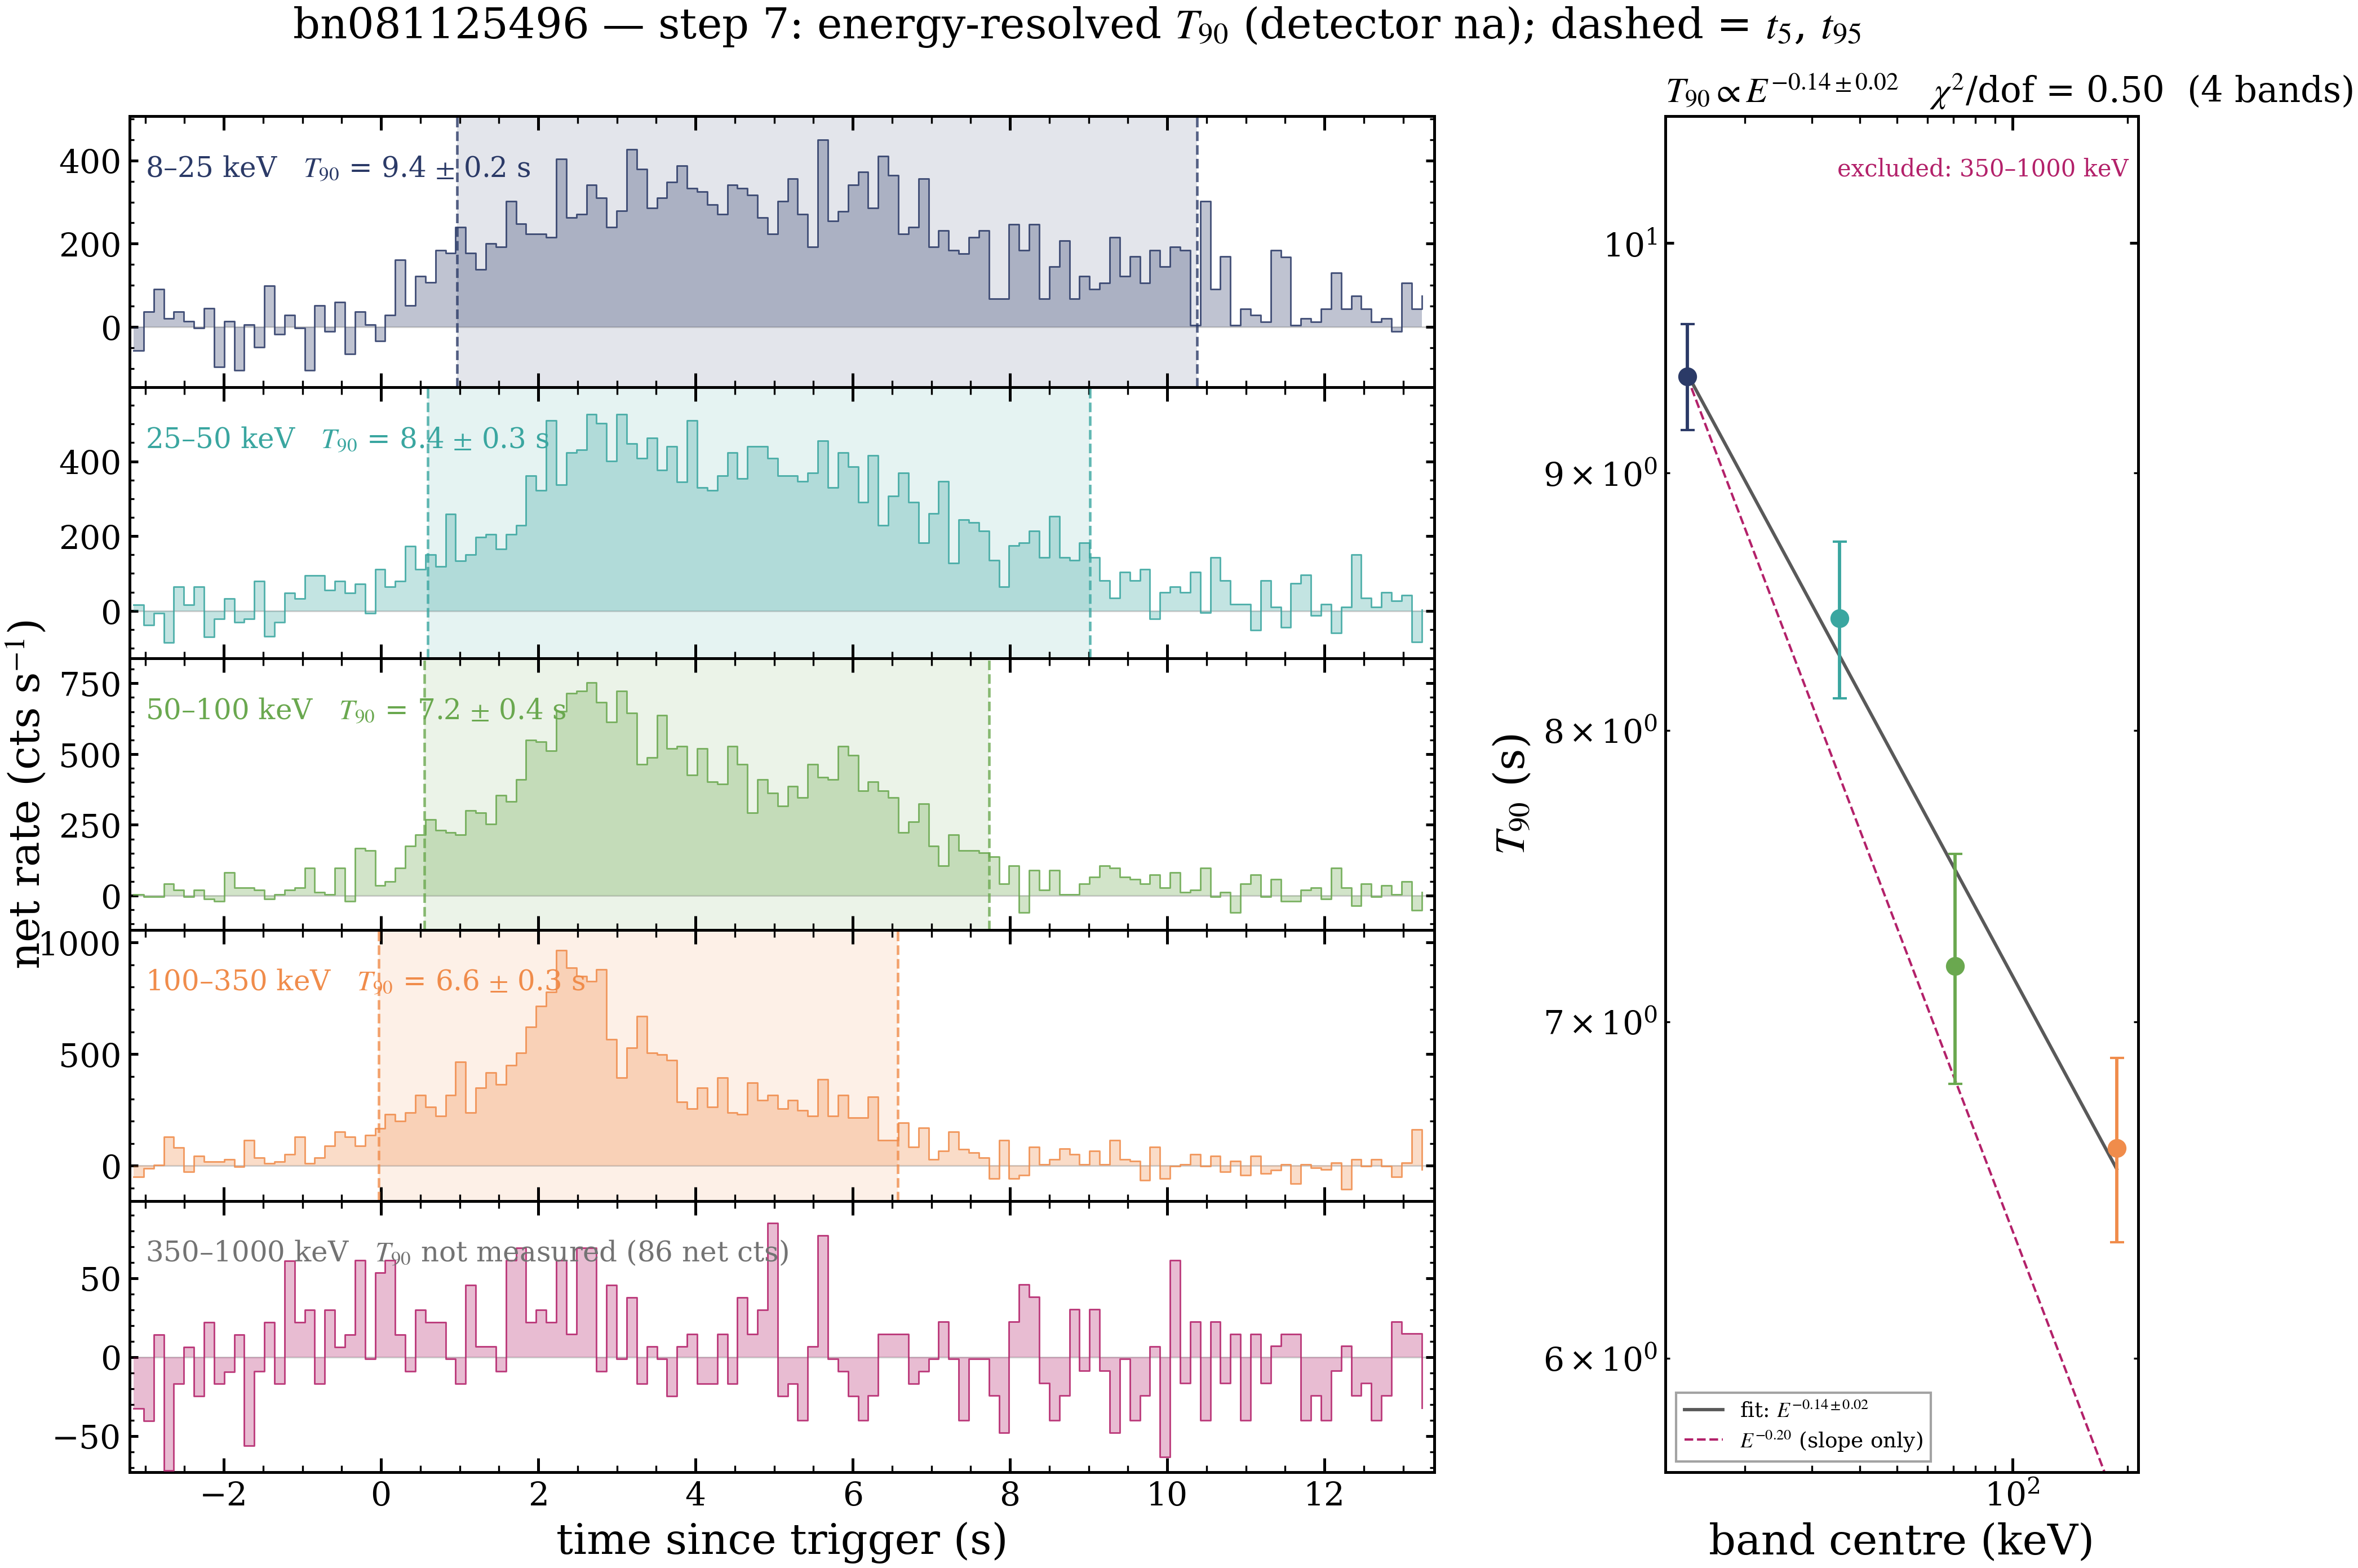
\includegraphics[width=\textwidth]{figs/bn081125496_step7_temporal.png}
\caption{Per-band light curves with individual $T_{90}$ measurements
(shaded $t_5$--$t_{95}$ spans; the 350--1000~keV band is excluded for
insufficient counts) and the $T_{90}(E)$ relation with the
\citet{2013ApJ...763...15Q} population slope for reference.
\label{fig:step7}}
\end{figure*}

\subsection{Pulse Shape} \label{sec:pulse}

We fit three analytic pulse models to the 8--900~keV net light curve
(Figure~\ref{fig:pulse}): the FRED form of \citet{1996ApJ...459..393N}, the
\citet{2003ApJ...596..389K} profile, and the two-sigmoid of
\citet{2025ApJ...991..230G}. The Kocevski profile wins
($\chi^2_r = 1.04$; Norris 1.08). The Gowri two-sigmoid, fitted under the
protocol of that paper ($r_l \le r_r$, $R^2 = 0.961 \ge 0.7$), gives the
shape parameter $\varphi = s_l/s_r = 0.317 \pm 0.026$: a clean FRED-like
asymmetry. We note $\varphi$ is a sigmoid-width ratio and is not directly
comparable to rise/decay-time asymmetries.

\begin{figure}
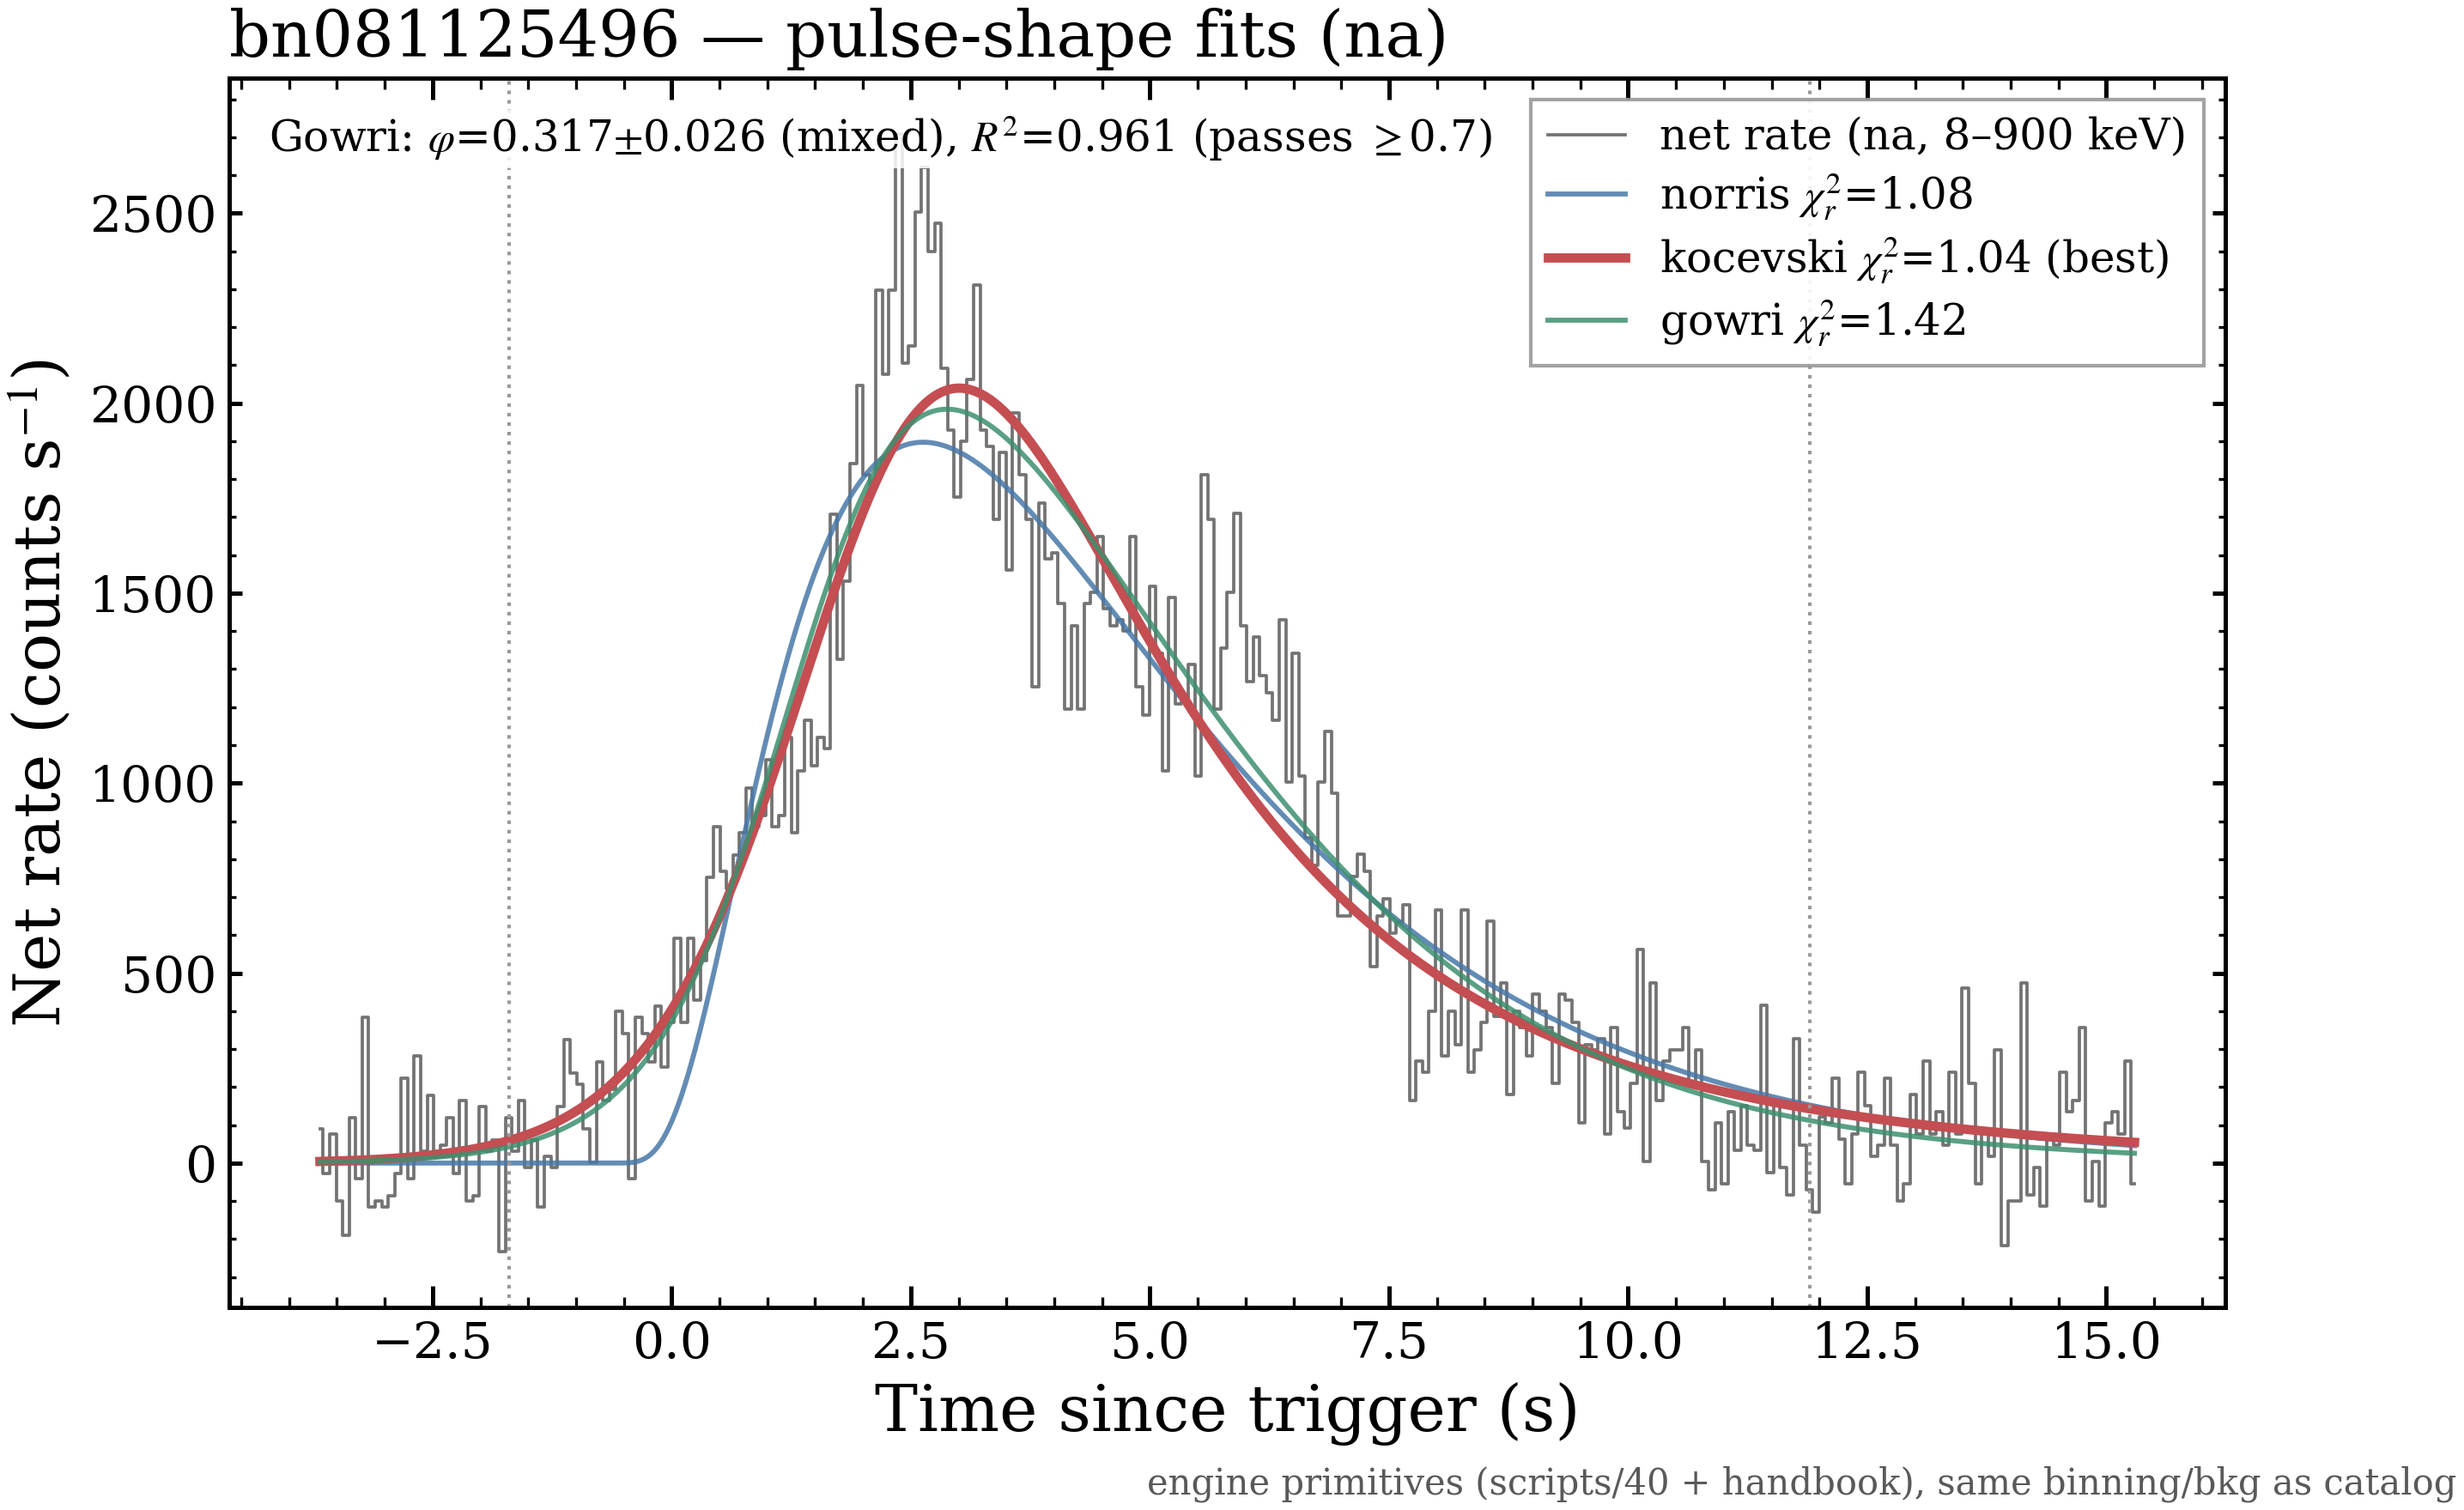
\includegraphics[width=\columnwidth]{figs/bn081125496_step7_pulse.png}
\caption{Pulse-shape fits to the net 8--900~keV light curve. The Kocevski
profile is the $\chi^2_r$ winner; the Gowri two-sigmoid supplies the
asymmetry parameter $\varphi$. \label{fig:pulse}}
\end{figure}

\subsection{Minimum Variability Timescale} \label{sec:mvt}

We measure the MVT with three estimators that differ at the primitive, and we
report all three with labels because they answer different questions
(Figure~\ref{fig:mvt}):

\begin{enumerate}
\item \textit{Windowed (canonical):} the validated framework of
\citet{2026ApJ...999...51B}, which scans short segments across the burst,
finds $33.9 \pm 2.9$~ms, localized on the pulse rise
(Figure~\ref{fig:balamvt}). The quoted uncertainty is the per-fit error; an
independent re-run shows realization scatter beyond it, and the local
detection $z$-score is 2.5 (weighted-mean significance 6.2) --- we therefore
quote this as the burst's MVT with those caveats attached.
\item \textit{Global CWT:} the continuous-wavelet method of
\citet{2018ApJ...864..163V} applied to the full source window returns
$215 \pm 17$~ms --- the timescale at which the \emph{whole window's} power
exceeds its Poisson floor.
\item \textit{Global Haar:} a Haar-wavelet structure minimum
\citep[cf.][]{2014ApJ...787...90G,2013MNRAS.432..857M} returns
$546 \pm 69$~ms.
\end{enumerate}

The ordering is not a discrepancy but a scope statement: a smooth 8.5~s FRED
dominates any global spectrum, while only a windowed scan can isolate the
$\sim$30~ms structure on the rise. Population studies that mix MVT estimators
mix questions; the energy dependence of MVT \citep{2015ApJ...811...93G}
compounds this across instruments.

\begin{figure}
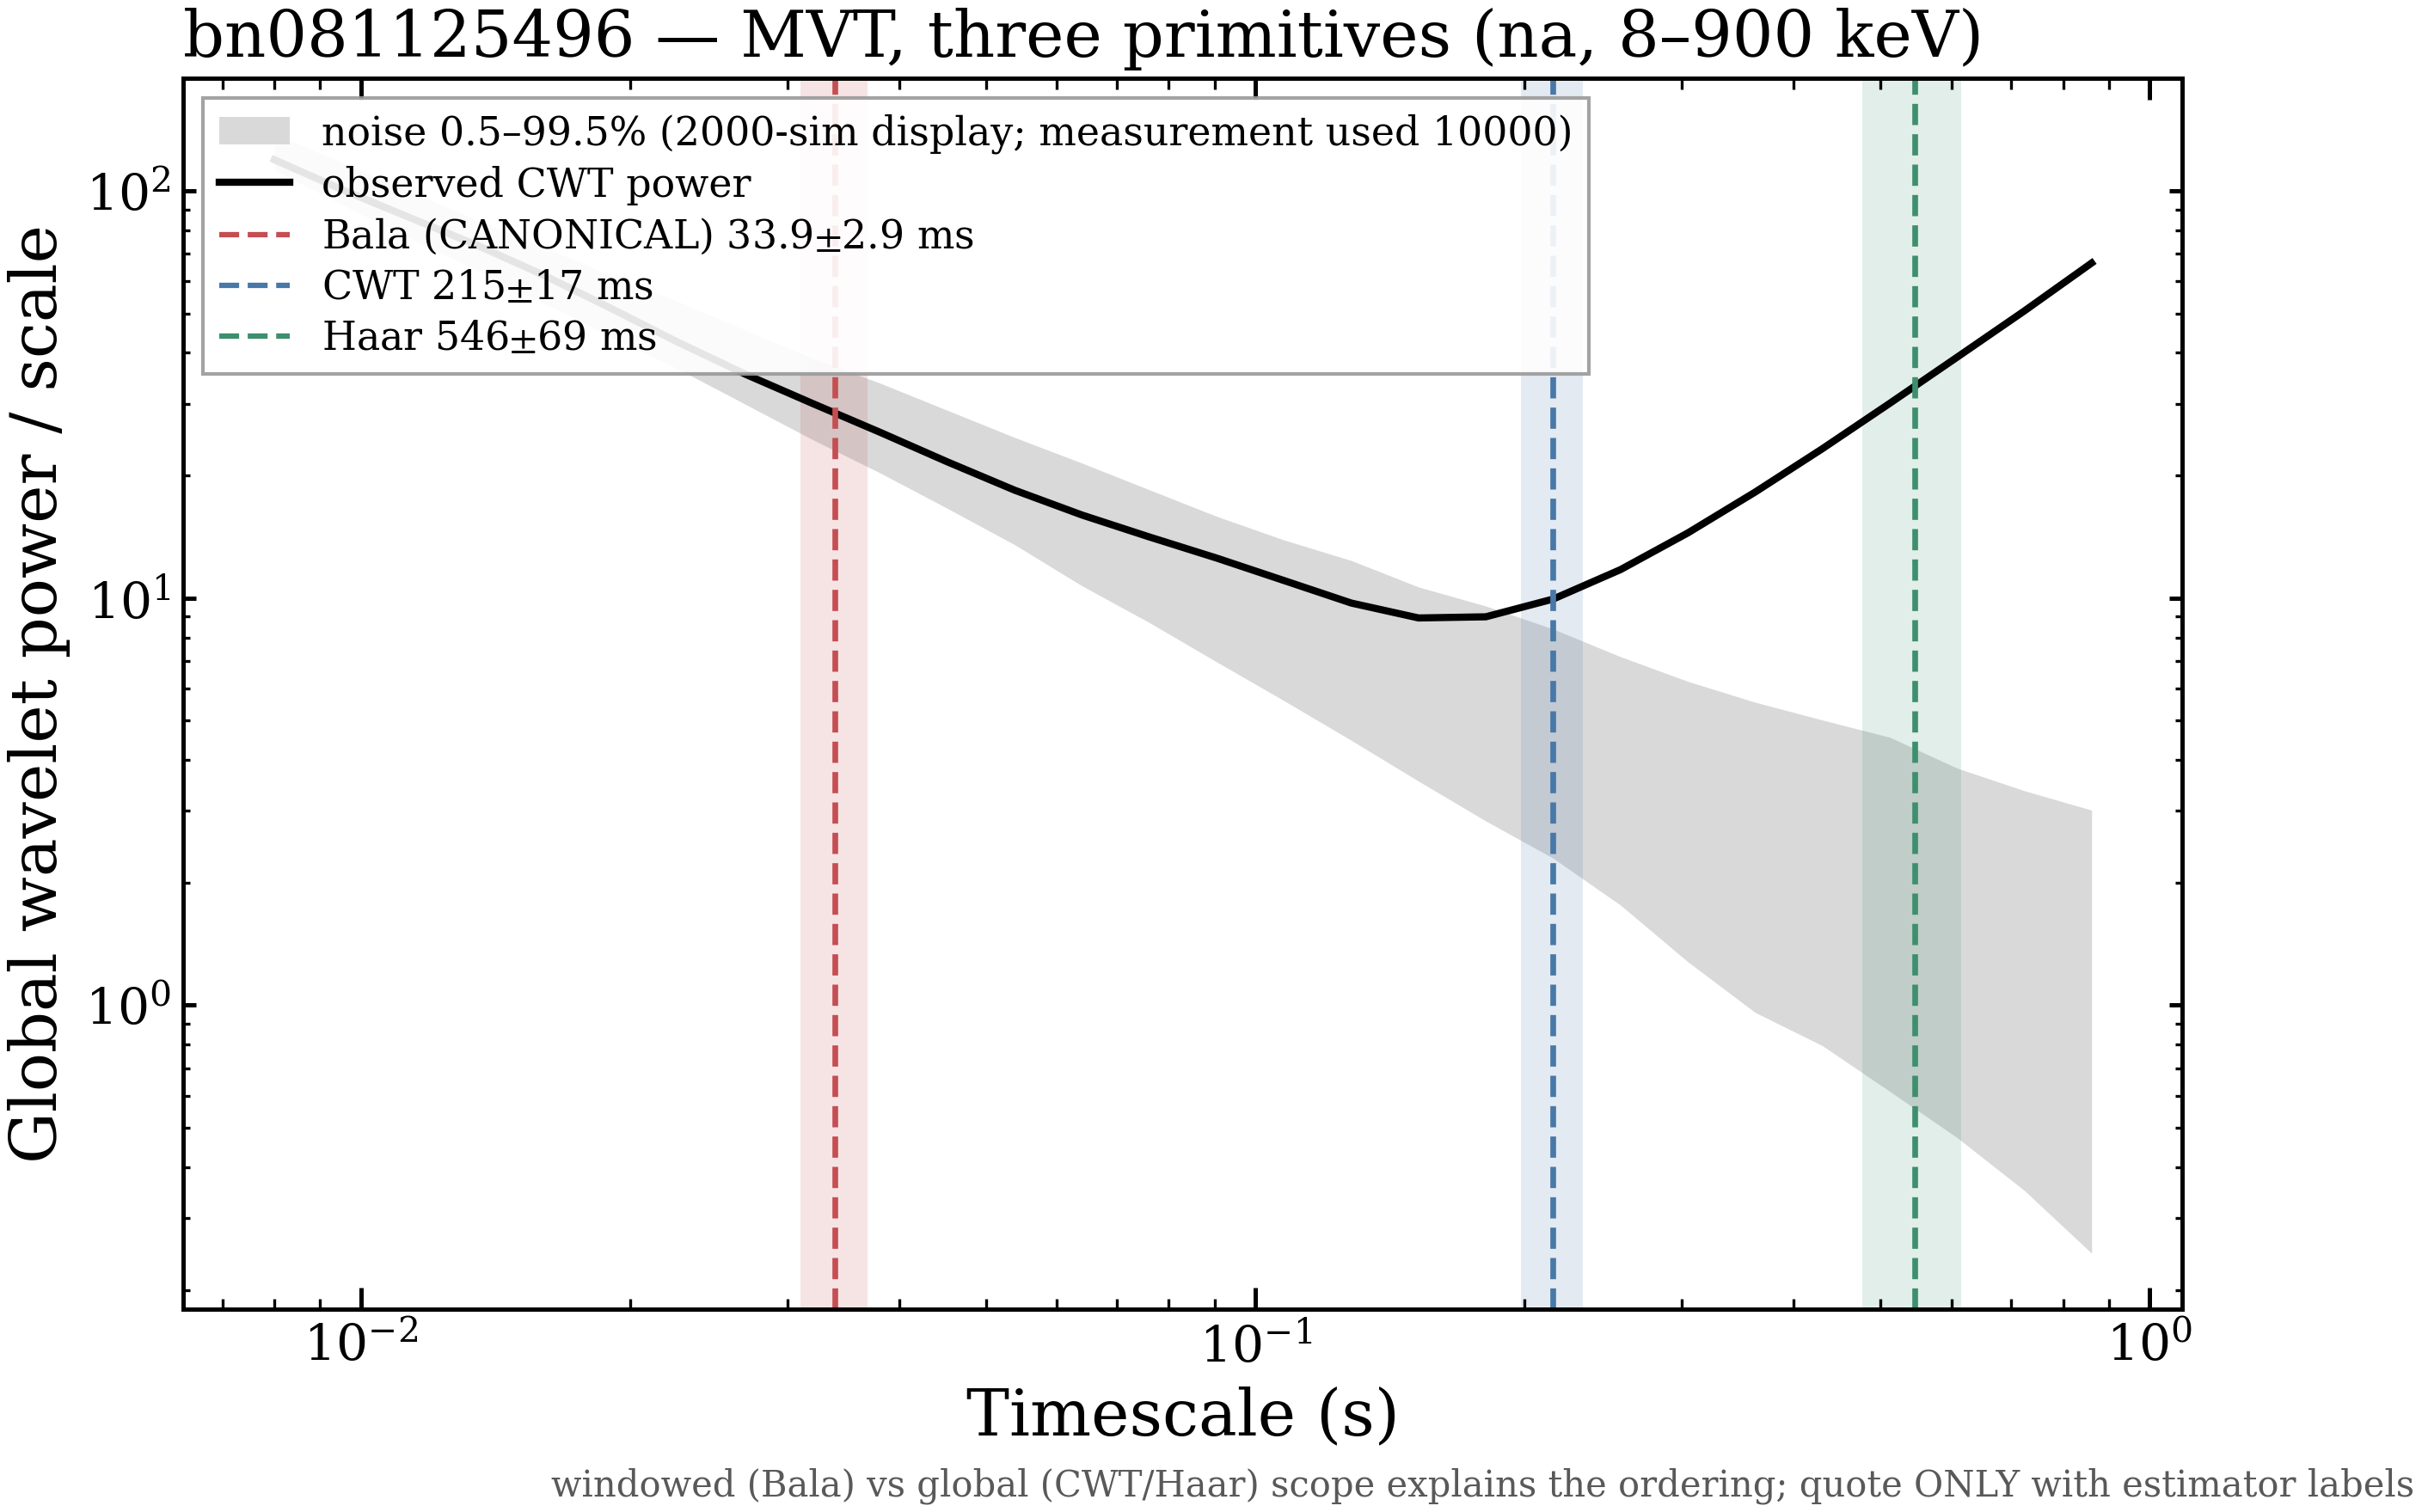
\includegraphics[width=\columnwidth]{figs/bn081125496_step7_mvt.png}
\caption{Global continuous-wavelet power spectrum of the \grb\ source
window (black) against the 0.5--99.5\% envelope of $10^4$ Poisson
realizations (gray), with all three MVT estimates marked (dashed lines with
$1\sigma$ bands). The global MVT is the scale at which observed power exits
the noise envelope --- a characteristic timescale closer to the rise time of
the shortest structures than to the shortest observable bin
\citep{2014ApJ...787...90G}. The windowed estimate (red) probes rise
structure that the whole-window spectrum averages away; the Haar minimum
(green) applies a later threshold on the same data. \label{fig:mvt}}
\end{figure}

\begin{figure}
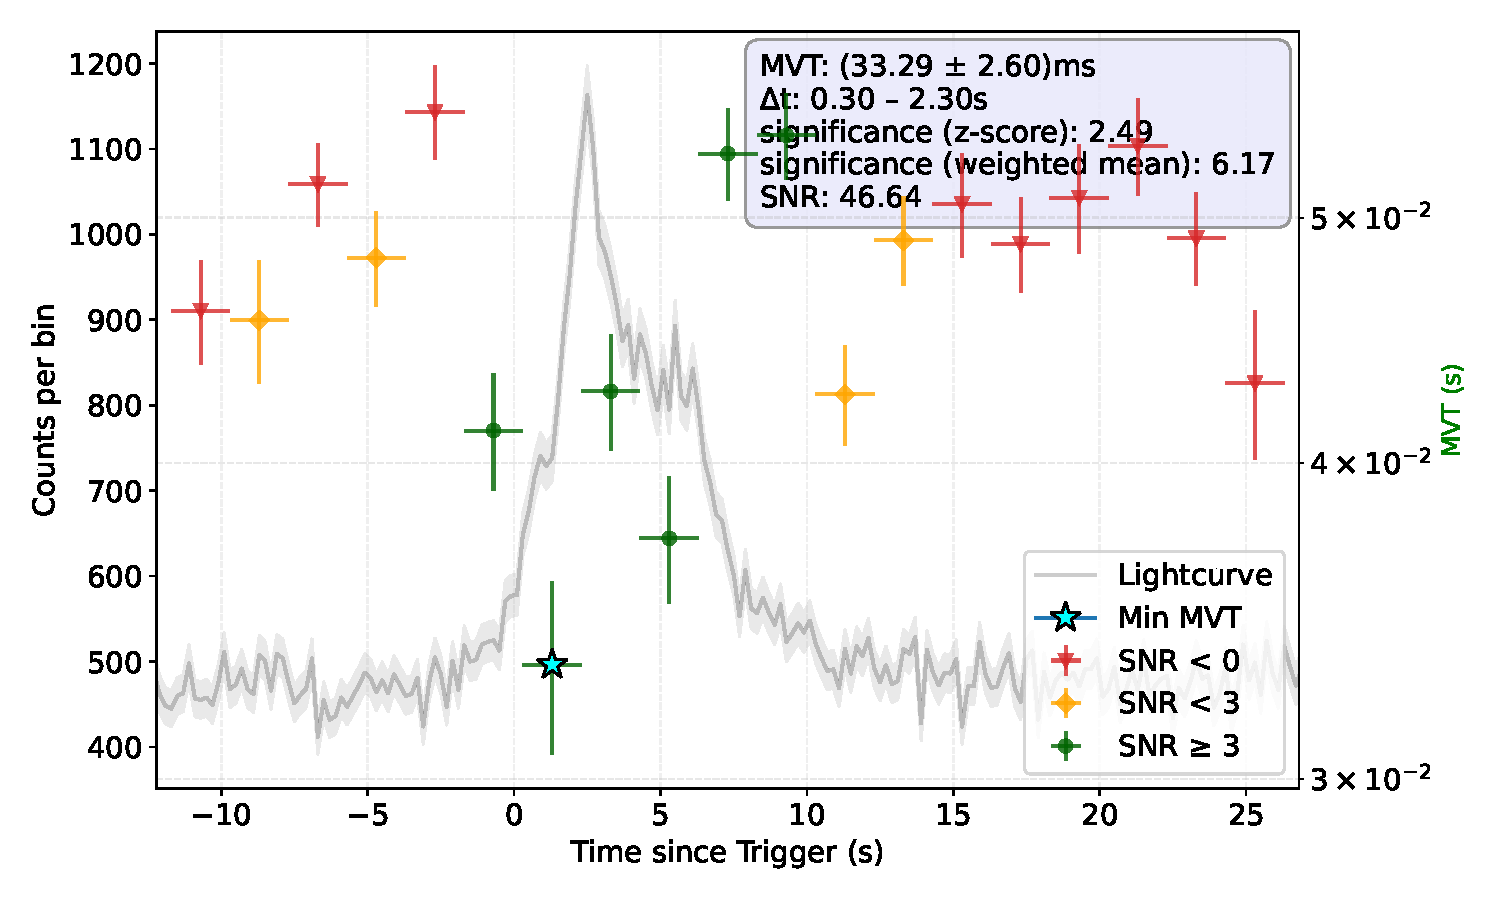
\includegraphics[width=\columnwidth]{figs/bala_mvt_native.pdf}
\caption{Native diagnostic of the windowed MVT framework
\citep{2026ApJ...999...51B}: MVT per 2~s segment over the light curve,
color-coded by segment signal-to-noise. The minimum ($33.3 \pm 2.6$~ms in
this realization) lies on the pulse rise; background-dominated segments (red)
trace the counting-noise ceiling, not the burst. \label{fig:balamvt}}
\end{figure}

\subsection{Spectral Lag} \label{sec:lag}

We measure the 25--50 vs.\ 100--300~keV lag with the discrete
cross-correlation function \citep{1997ApJ...486..928B}, an asymmetric-Gaussian
peak model \citep{2015MNRAS.446.1129B}, and flux-randomization Monte Carlo
errors \citep{1998PASP..110..660P}, taking the MC median with 16/84-percentile
uncertainties: $\tau = 0.705^{+0.291}_{-0.205}$~s, soft lagging hard
(positive lag in the standard convention;
\citealt{1996ApJ...459..393N,2010ApJ...711.1073U}), with a $39\sigma$ CCF
peak (Figure~\ref{fig:lag}).\footnote{An earlier in-house lag product was
quarantined after failing sign-convention validation against the standard
Norris definition; the defect and its resolution are recorded in the campaign
ledger.}

For a single broad pulse this number requires interpretation. The soft and
hard light curves are near-copies of one envelope, so the CCF is a broad
function whose width is set by the pulse duration; its peak offset measures
the soft--hard shift of the envelope --- the FRED's hard-to-soft evolution
--- not a photon arrival delay. Consistently, $\tau/T_{90} \approx 0.08$,
in line with lag--width scaling within the pulse paradigm
\citep{1996ApJ...459..393N,2012MNRAS.419..614U}. This has a population
consequence: in lag--variability correlations
\citep{2013ApJ...778....3S,2025JARNA..11...27G}, pulse width can enter both
axes for broad-pulse bursts, and single-pulse samples with width-scaled
windows (this campaign) are the clean way to separate the physics from the
scaling.

\begin{figure}
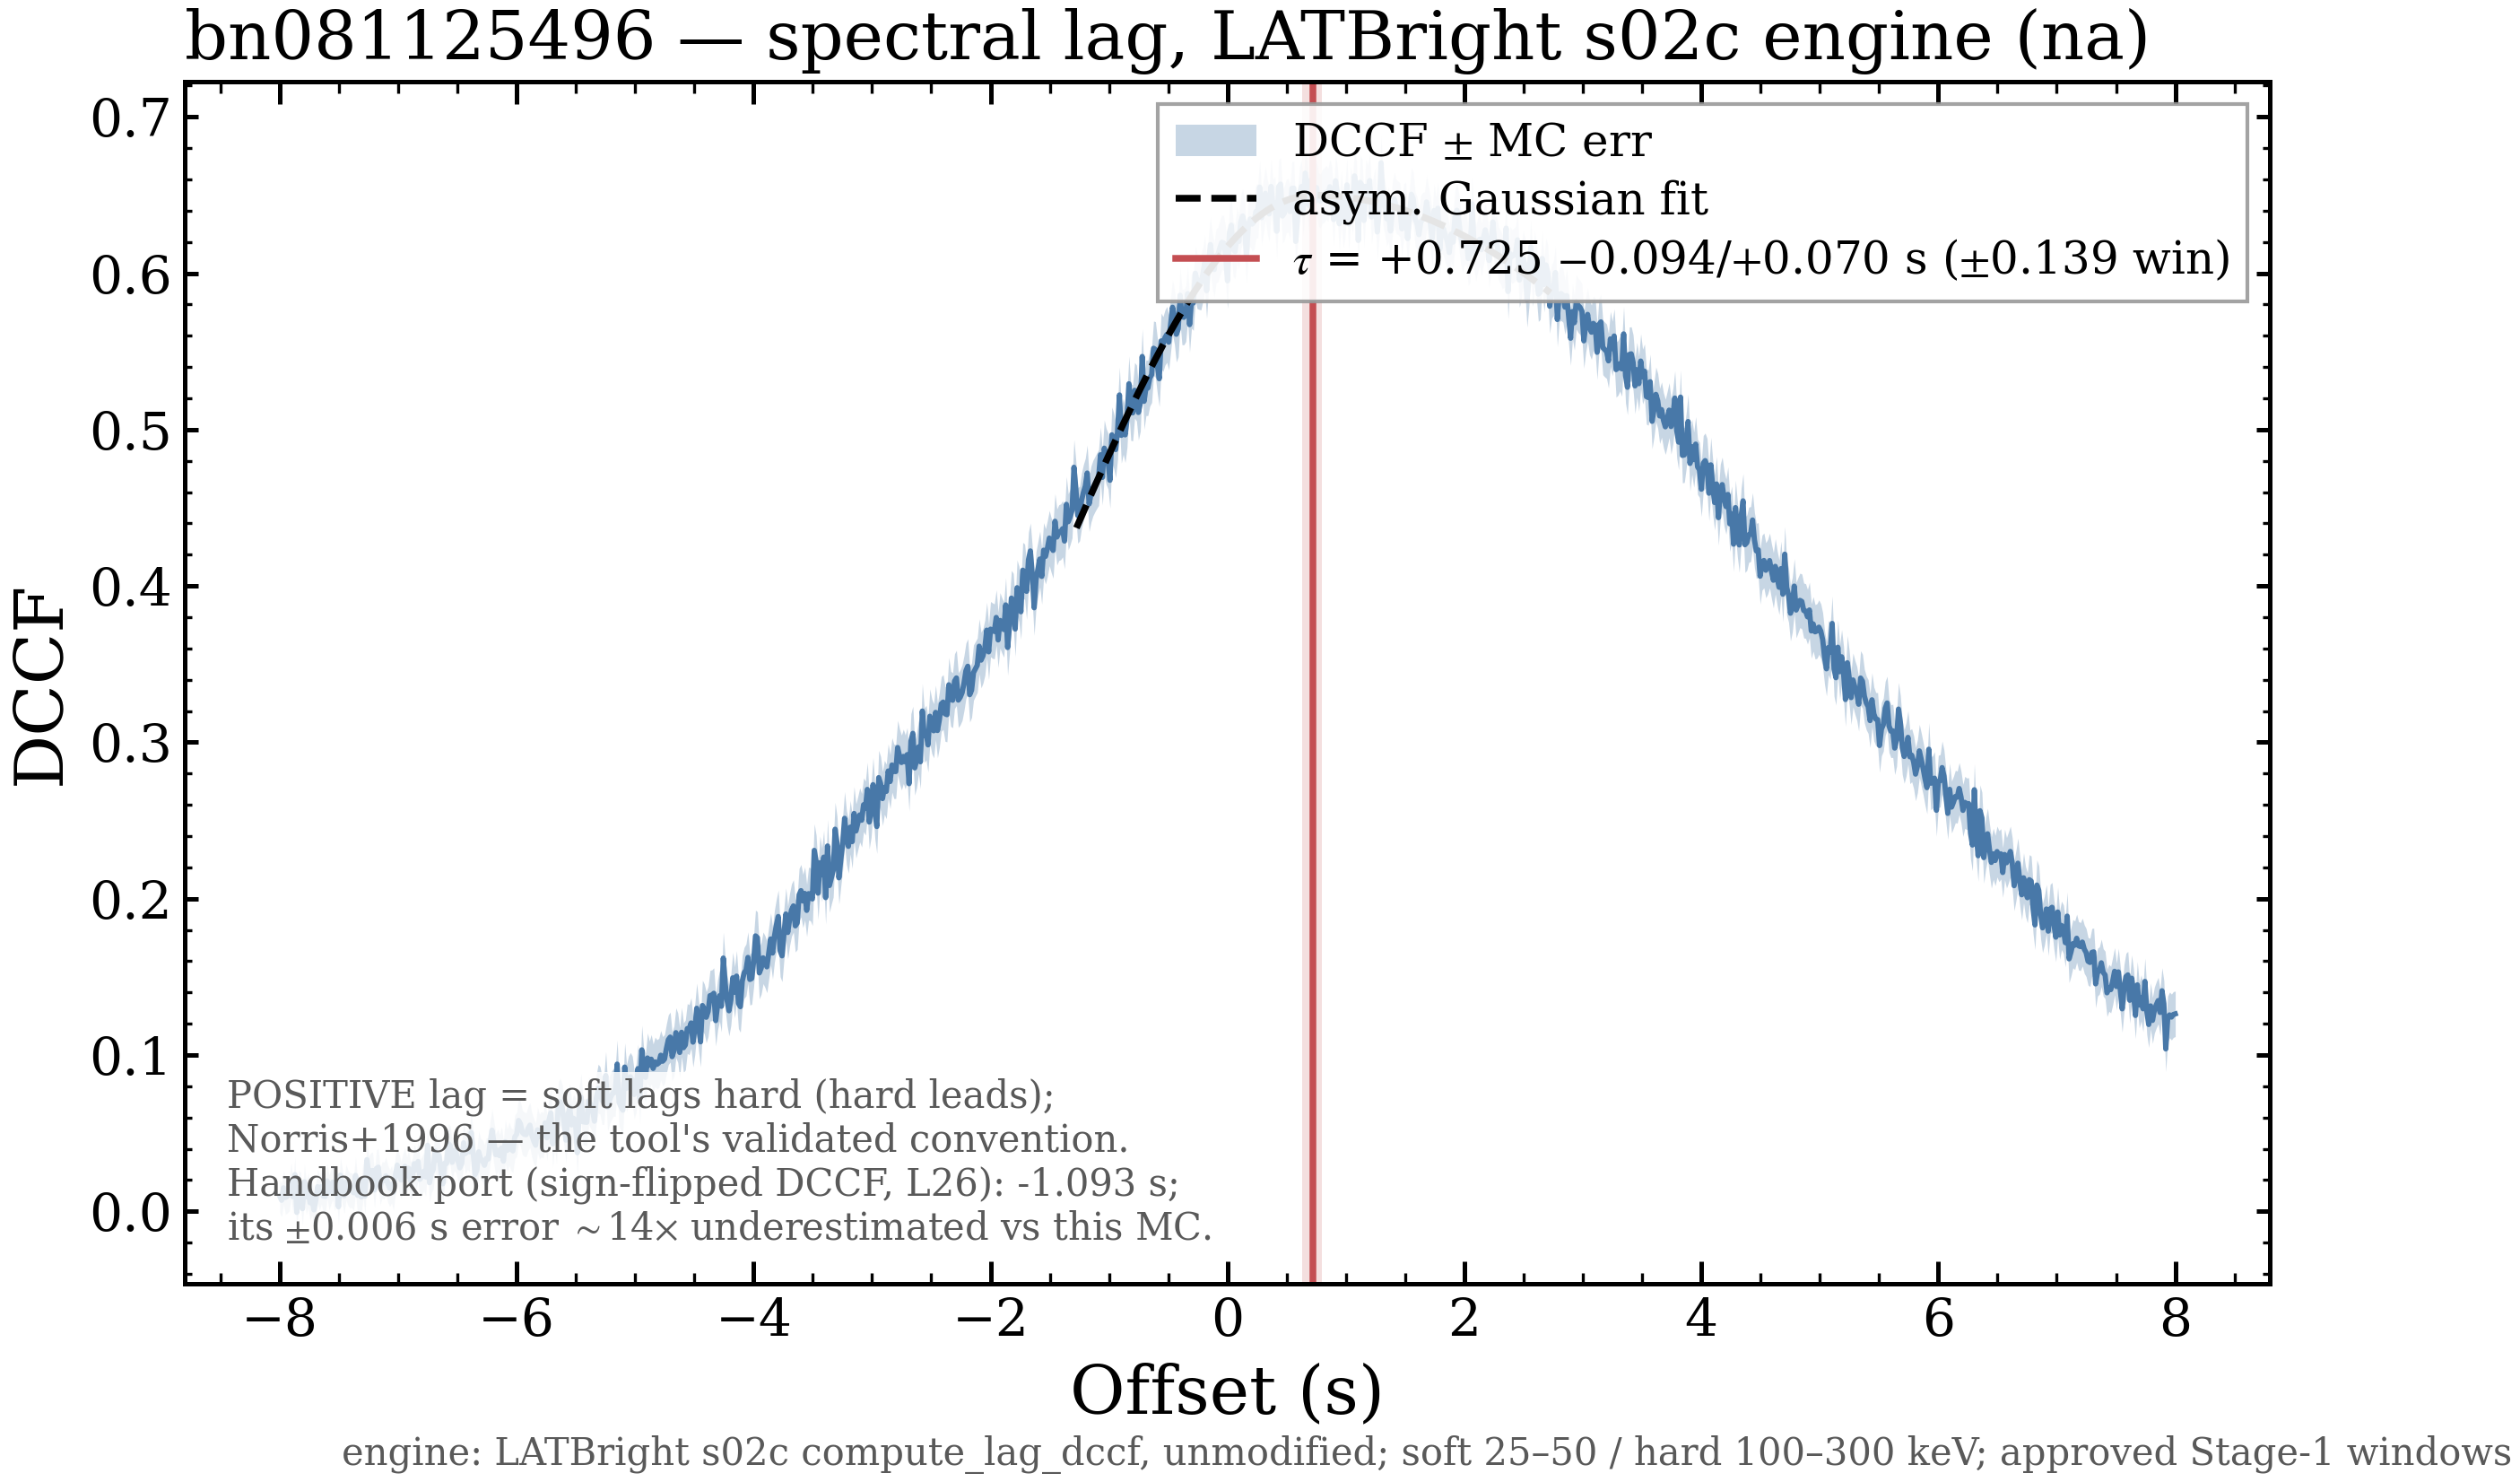
\includegraphics[width=\columnwidth]{figs/bn081125496_step7_lag_latbright.png}
\caption{Discrete cross-correlation of the 25--50 and 100--300~keV light
curves with the asymmetric-Gaussian peak model and the MC-median lag
(positive $=$ soft lags hard). For a single broad FRED the CCF width is the
pulse width; the lag measures envelope evolution
(\S\ref{sec:lag}). \label{fig:lag}}
\end{figure}


\section{Time Binning} \label{sec:binning}

We bin the source window with Bayesian blocks \citep{2013ApJ...764..167S} run
through the Multi-Mission Maximum Likelihood framework
\citep[3ML;][]{2015arXiv150708343V}, followed by a significance-based merge
requiring $S \ge 10$ per bin on the reference detector
\citep[cf.][who apply $S \ge 20$ to detector-combined spectra;
the single-detector floor is comparable after the $\sqrt{M}$
correction]{2019ApJ...886...20Y}. This yields nine time bins spanning
$-1.70$ to $10.65$~s (Figure~\ref{fig:step5}).

\begin{figure}
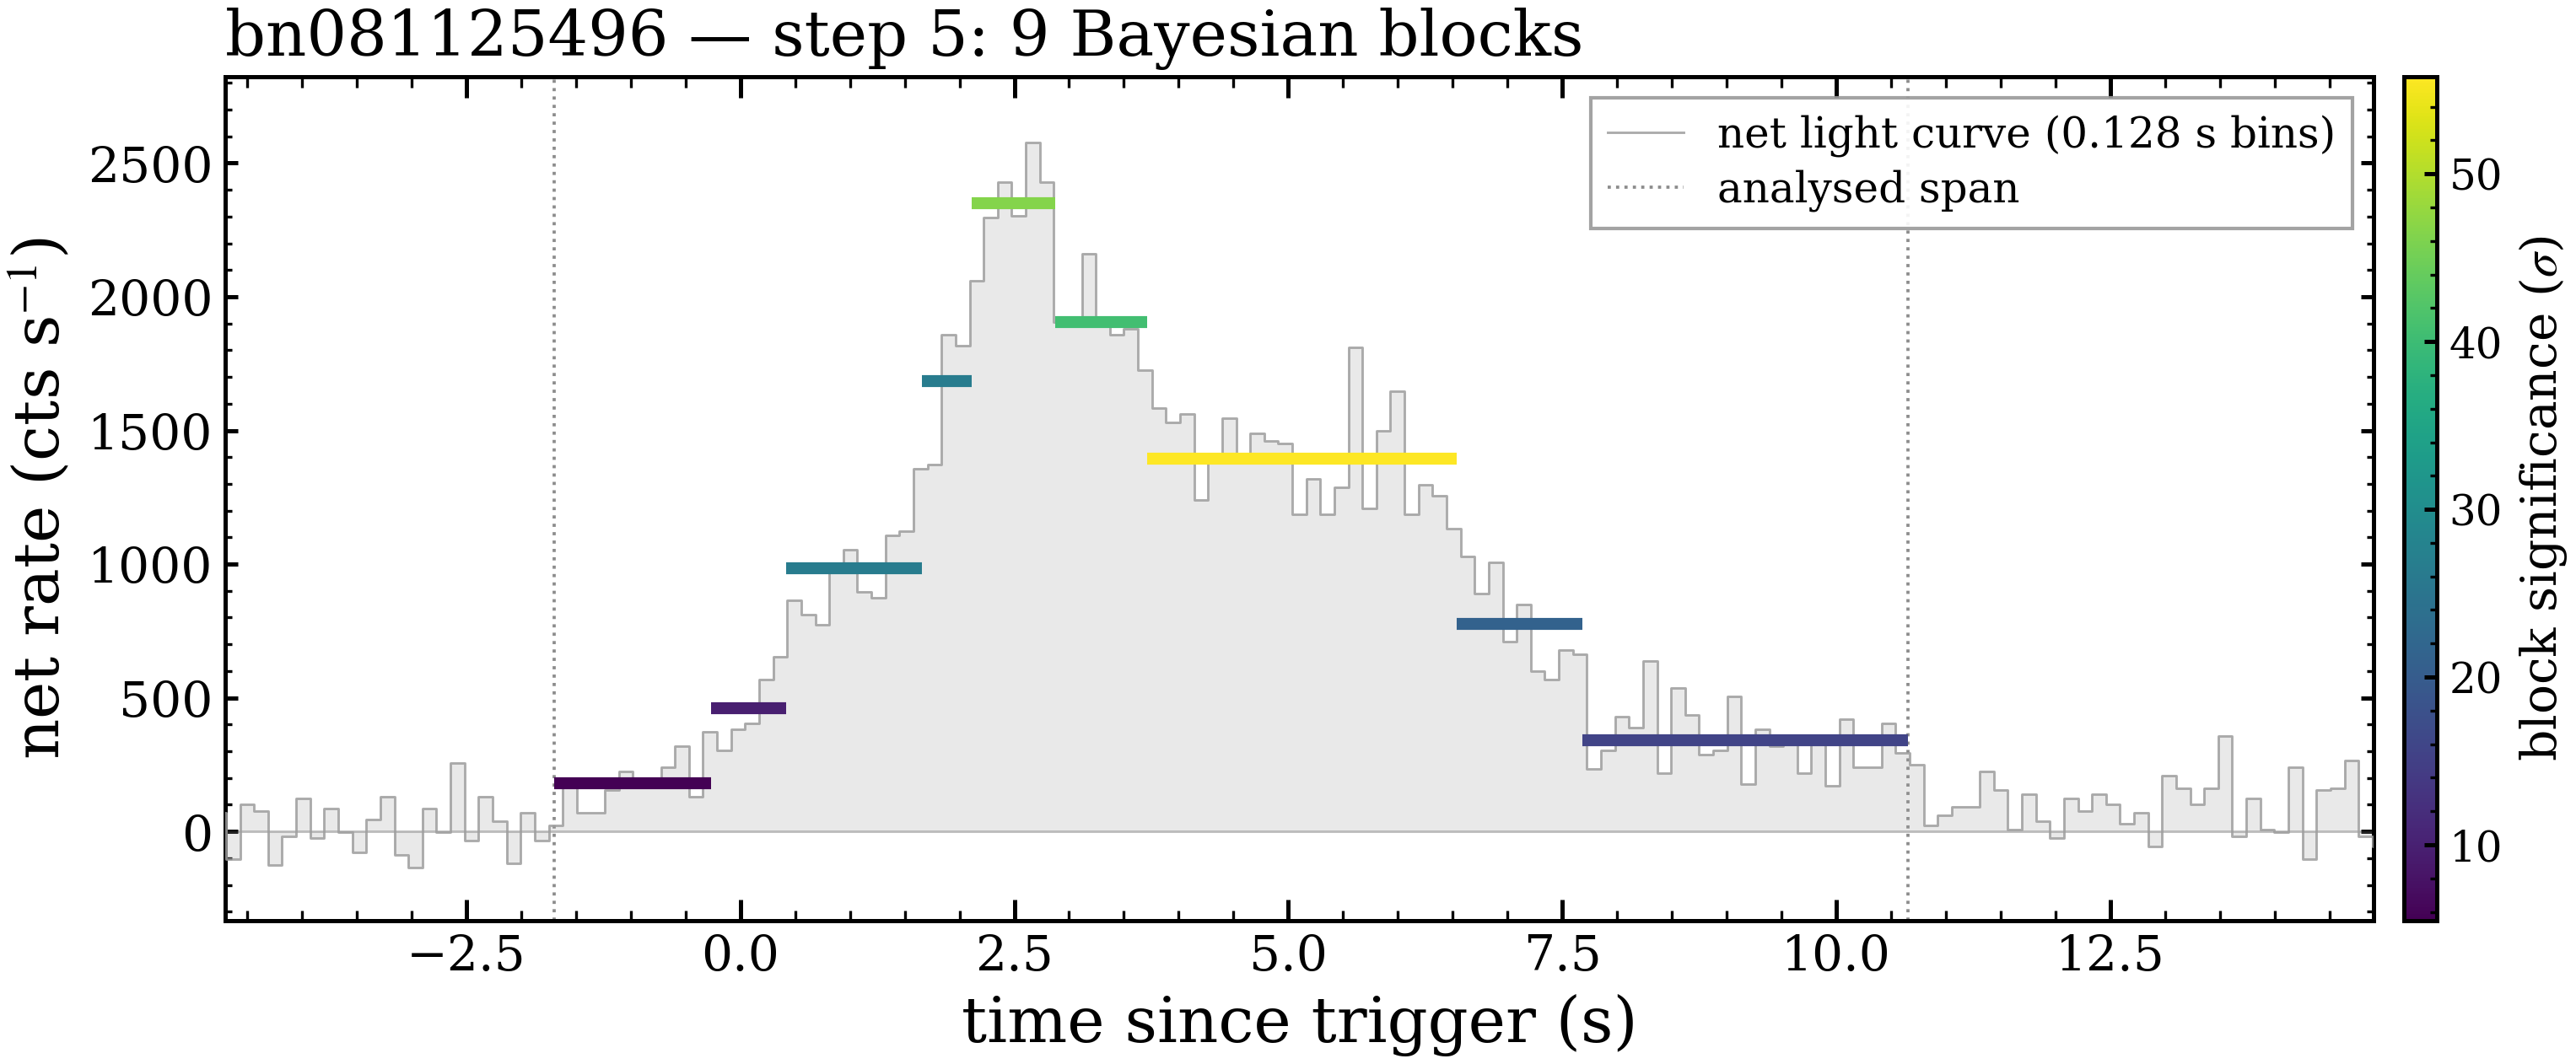
\includegraphics[width=\columnwidth]{figs/bn081125496_step5_binning.png}
\caption{Time binning for \grb. The Bayesian-block decomposition of the
reference-detector light curve \citep{2013ApJ...764..167S} is merged to the
nine spectroscopy bins (shaded spans) by the $S \ge 10$ significance floor;
block edges are drawn from the reference NaI. \label{fig:step5}}
\end{figure}

\section{Time-Resolved Spectroscopy} \label{sec:spectra}

\subsection{Method} \label{sec:specmethod}

For each of the nine bins and the time-integrated (T$_{\rm INT}$) spectrum we
fit 24 spectral models: the standard single-continuum forms (power law, cutoff
power law, Band, smoothly broken power law, double smoothly broken power law
\citep[cf.][]{1993ApJ...413..281B,2019A&A...625A..60R}) and their combinations
with blackbody, power-law, and cutoff power-law components. Fits minimize the
Poisson--Gaussian likelihood ($\pgstat$) in 3ML with inter-detector effective
area corrections free within $[0.8, 1.2]$ for the non-reference detectors.
Model selection uses the Akaike Information Criterion
\citep[AIC;][]{1974ITAC...19..716A}; we treat $\Delta\mathrm{AIC} < 2$ as a
statistical tie. As a representative goodness measure, the time-integrated
winner has $\pgstat/\mathrm{dof} = 4226.4/342$.

\subsection{Results} \label{sec:specresults}

Table~\ref{tab:winners} lists the AIC winner and its parameters in every bin.
Figure~\ref{fig:sedtint} and Figure~\ref{fig:sedbin4} show the two flagship
spectra --- the time-integrated Band fit and the peak-bin (bin 4) cutoff
power-law fit --- in $\nu F_\nu$ representation with data unfolded following
the XSPEC \texttt{eeufspec} construction (group-integrated ratio unfolding),
68\% error bands from 3ML's native error propagation, and count-space
residuals. Figure~\ref{fig:montage} shows all 24 model fits for the
time-integrated spectrum in a single AIC-ordered montage; equivalent montages
for every bin are provided in Appendix~\ref{app:montages}.

The spectral story is compact:

\textit{A cutoff power law suffices almost everywhere.} CPL wins six of nine
resolved bins (Table~\ref{tab:winners}); in those bins every added component
either rails to a boundary or reproduces the CPL shape. The margins to the
runner-up are thin throughout ($\Delta\mathrm{AIC} = 0.3$--$2.0$): this is a
burst in which many shapes tie, and we report winners with that caveat.

\textit{A high-energy tail is demanded only on the rise and in the late
tail.} In bin~2 (the pulse rise) a pure cutoff leaves a coherent positive run
across six of seven BGO groups at 0.3--10~MeV, and Band-family models absorb
it ($\beta = -2.08^{+0.13}_{-0.19}$). In bin~8 (the late tail) the tail
demand returns decisively (Band $\beta = -2.18^{+0.17}_{-0.26}$,
$E_{\rm p} = 37^{+16}_{-7}$~keV). In between, the tail is absent or
sub-threshold. The models tied at $\Delta\mathrm{AIC} < 1$ in bin~8 disagree
by an order of magnitude in 30~MeV flux: high-energy extrapolations from this
burst are model-dominated and we do not quote them.

\textit{The time-integrated winner is an artifact of evolution.} The
smoothly broken power law plus power law wins T$_{\rm INT}$
($\mathrm{AIC} = 4242.4$, a statistical dead heat with three other
composites) but wins \emph{no} resolved bin, and its power-law component is
invalid (railed) in eight of nine bins. Integrating a spectrum whose cutoff
energy evolves by a factor $\gtrsim 5$ (Figure~\ref{fig:evoCPL}) manufactures an
apparent second component. This is a concrete, single-burst demonstration of
why time-integrated component claims require time-resolved confirmation.

\textit{No photospheric component.} Across $\sim$90 blackbody-added fits in
all bins we find zero thermal evidence. The fitted blackbody population is
bimodal: a $kT \simeq 1.1$--$1.9$~keV cluster whose Wien peak
($3.92\,kT \lesssim 7.5$~keV) lies \emph{below} the 8~keV fitted boundary ---
edge-constrained artifacts absorbing low-energy calibration structure, not
photospheres --- and a $kT \simeq 10$--$40$~keV cluster with normalizations
consistent with zero. The bin-2 AIC winner (Band+BB,
$kT = 1.55^{+0.51}_{-0.37}$~keV) is itself the cautionary case: an
edge-constrained feature at the top of a ranking table. We flag such
solutions by the criterion $3.92\,kT$ below the fitted band and exclude them
from any thermal census.

\textit{Inter-detector calibration.} The $n_b$ effective-area factor rests on
its 0.8 lower bound in five of nine bins (e.g., $0.8134 \pm 0.034$ in bin~4);
$b_1$ reaches 1.2 in two. The bounds are held fixed at $[0.8, 1.2]$ as a
calibration prior. Low-energy features in this burst inherit that caveat,
which is one reason the edge-constrained blackbodies above are not read as
physical.

\begin{deluxetable*}{lccccl}
\tablecaption{AIC-selected best model per time bin (statistical ties at
$\Delta\mathrm{AIC}<2$ are noted in the text). Errors are MINOS
asymmetric. \label{tab:winners}}
\tablehead{
\colhead{Bin} & \colhead{Interval (s)} & \colhead{Model} &
\colhead{AIC} & \colhead{$\Delta$AIC$_{\rm 2nd}$} & \colhead{Parameters}
}
\startdata
T$_{\rm INT}$ & $[-1.70, 10.65]$ & SBPL+PL & 4242.4 & 0.8 &
$\alpha=-0.31^{+0.38}_{-0.35}$, $E_{\rm b}=146^{+58}_{-38}$,
$\beta=-3.35^{+0.39}_{-0.54}$; PL: $-1.63^{+0.63}_{-0.15}$ \\
0 & $[-1.70, -0.27]$ & CPL & 1966.9 & 2.0 &
$\Gamma=-0.23^{+0.61}_{-0.42}$, $E_{\rm c}=315^{+260}_{-130}$ \\
1 & $[-0.27, 0.42]$ & CPL & 1207.0 & 0.8 &
$\Gamma=-0.43^{+0.27}_{-0.22}$, $E_{\rm c}=321^{+170}_{-100}$ \\
2 & $[0.42, 1.66]$ & Band+BB\tablenotemark{a} & 1868.4 & 1.4 &
$\alpha=+0.02^{+0.31}_{-0.26}$, $E_{\rm p}=202^{+39}_{-28}$,
$\beta=-2.08^{+0.13}_{-0.19}$; $kT=1.55^{+0.51}_{-0.37}$ \\
3 & $[1.66, 2.11]$ & CPL & 813.1\tablenotemark{b} & 1.6 &
$\Gamma=-0.31^{+0.13}_{-0.12}$, $E_{\rm c}=167^{+30}_{-24}$ \\
4 & $[2.11, 2.87]$ & CPL & 1374.2 & 1.5 &
$\Gamma=-0.147^{+0.090}_{-0.085}$, $E_{\rm c}=134^{+13}_{-12}$ \\
5 & $[2.87, 3.71]$ & Band & 1482.2\tablenotemark{b} & 0.6 &
$\alpha=+0.08^{+0.17}_{-0.15}$, $E_{\rm p}=155^{+13}_{-12}$,
$\beta=-2.99^{+0.36}_{-0.65}$ \\
6 & $[3.71, 6.54]$ & CPL & 2717.9 & 1.9 &
$\Gamma=-0.305^{+0.074}_{-0.072}$, $E_{\rm c}=77.7^{+5.8}_{-5.1}$ \\
7 & $[6.54, 7.68]$ & CPL & 1675.6 & 0.8 &
$\Gamma=-0.48^{+0.24}_{-0.22}$, $E_{\rm c}=59^{+16}_{-12}$ \\
8 & $[7.68, 10.65]$ & Band & 2646.0 & 0.3 &
$\alpha=-0.10^{+1.4}_{-0.93}$, $E_{\rm p}=36.9^{+16}_{-6.9}$,
$\beta=-2.18^{+0.17}_{-0.26}$ \\
\enddata
\tablenotetext{a}{Edge-constrained blackbody: $3.92\,kT = 6.1$~keV lies below
the 8~keV fitted boundary; not photospheric (\S\ref{sec:specresults}).}
\tablenotetext{b}{AIC values are per-bin and not comparable across bins
(different data).}
\tablecomments{Energies in keV. All values provisional pending campaign
freeze. The complete 24-model $\times$ 10-bin parameter tables are available
as machine-readable products.}
\end{deluxetable*}

\begin{figure}
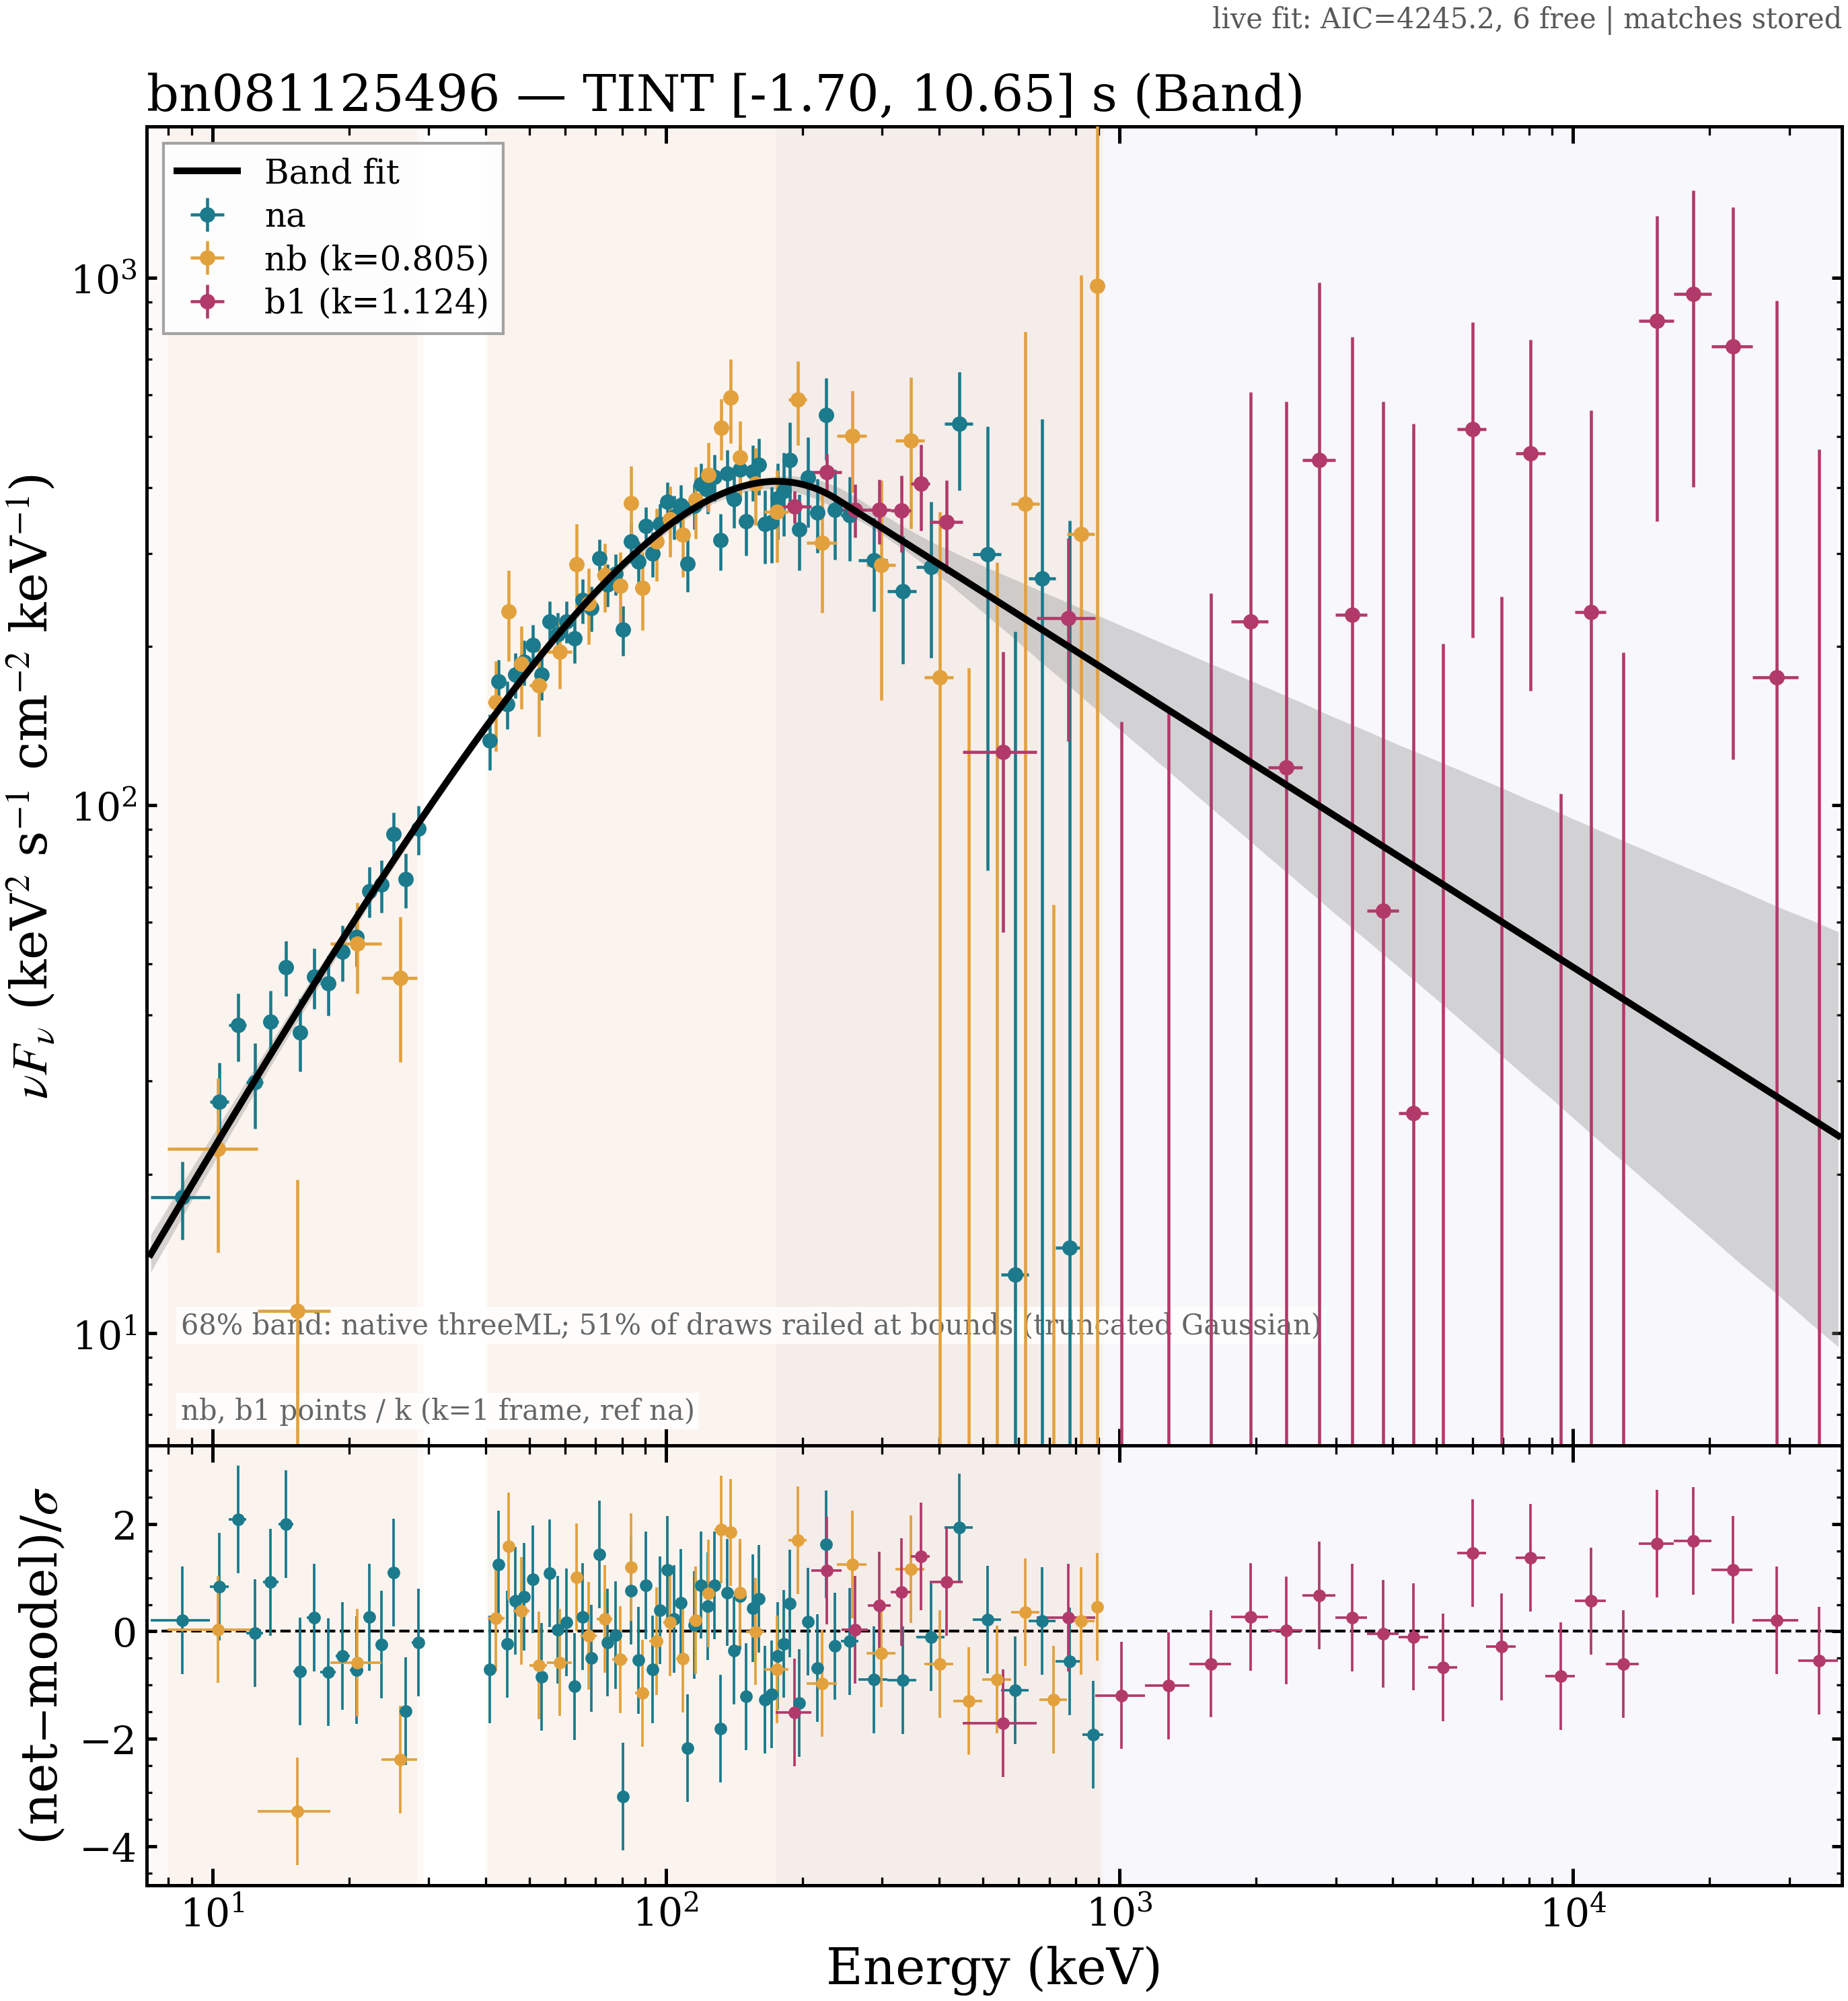
\includegraphics[width=\columnwidth]{figs/bn081125496_SED_TINT_Band.png}
\caption{Time-integrated $\nu F_\nu$ spectrum with the Band fit. Data points
are group-integrated ratio-unfolded (XSPEC \texttt{eeufspec} construction) at
\texttt{rebin 5 5}; non-reference detectors are scaled by their fitted
effective-area factors onto the $k=1$ frame (factors in legend); the 68\%
band is 3ML's native error propagation. Bottom: count-space residuals
$({\rm net}-{\rm model})/\sigma$. \label{fig:sedtint}}
\end{figure}

\begin{figure}
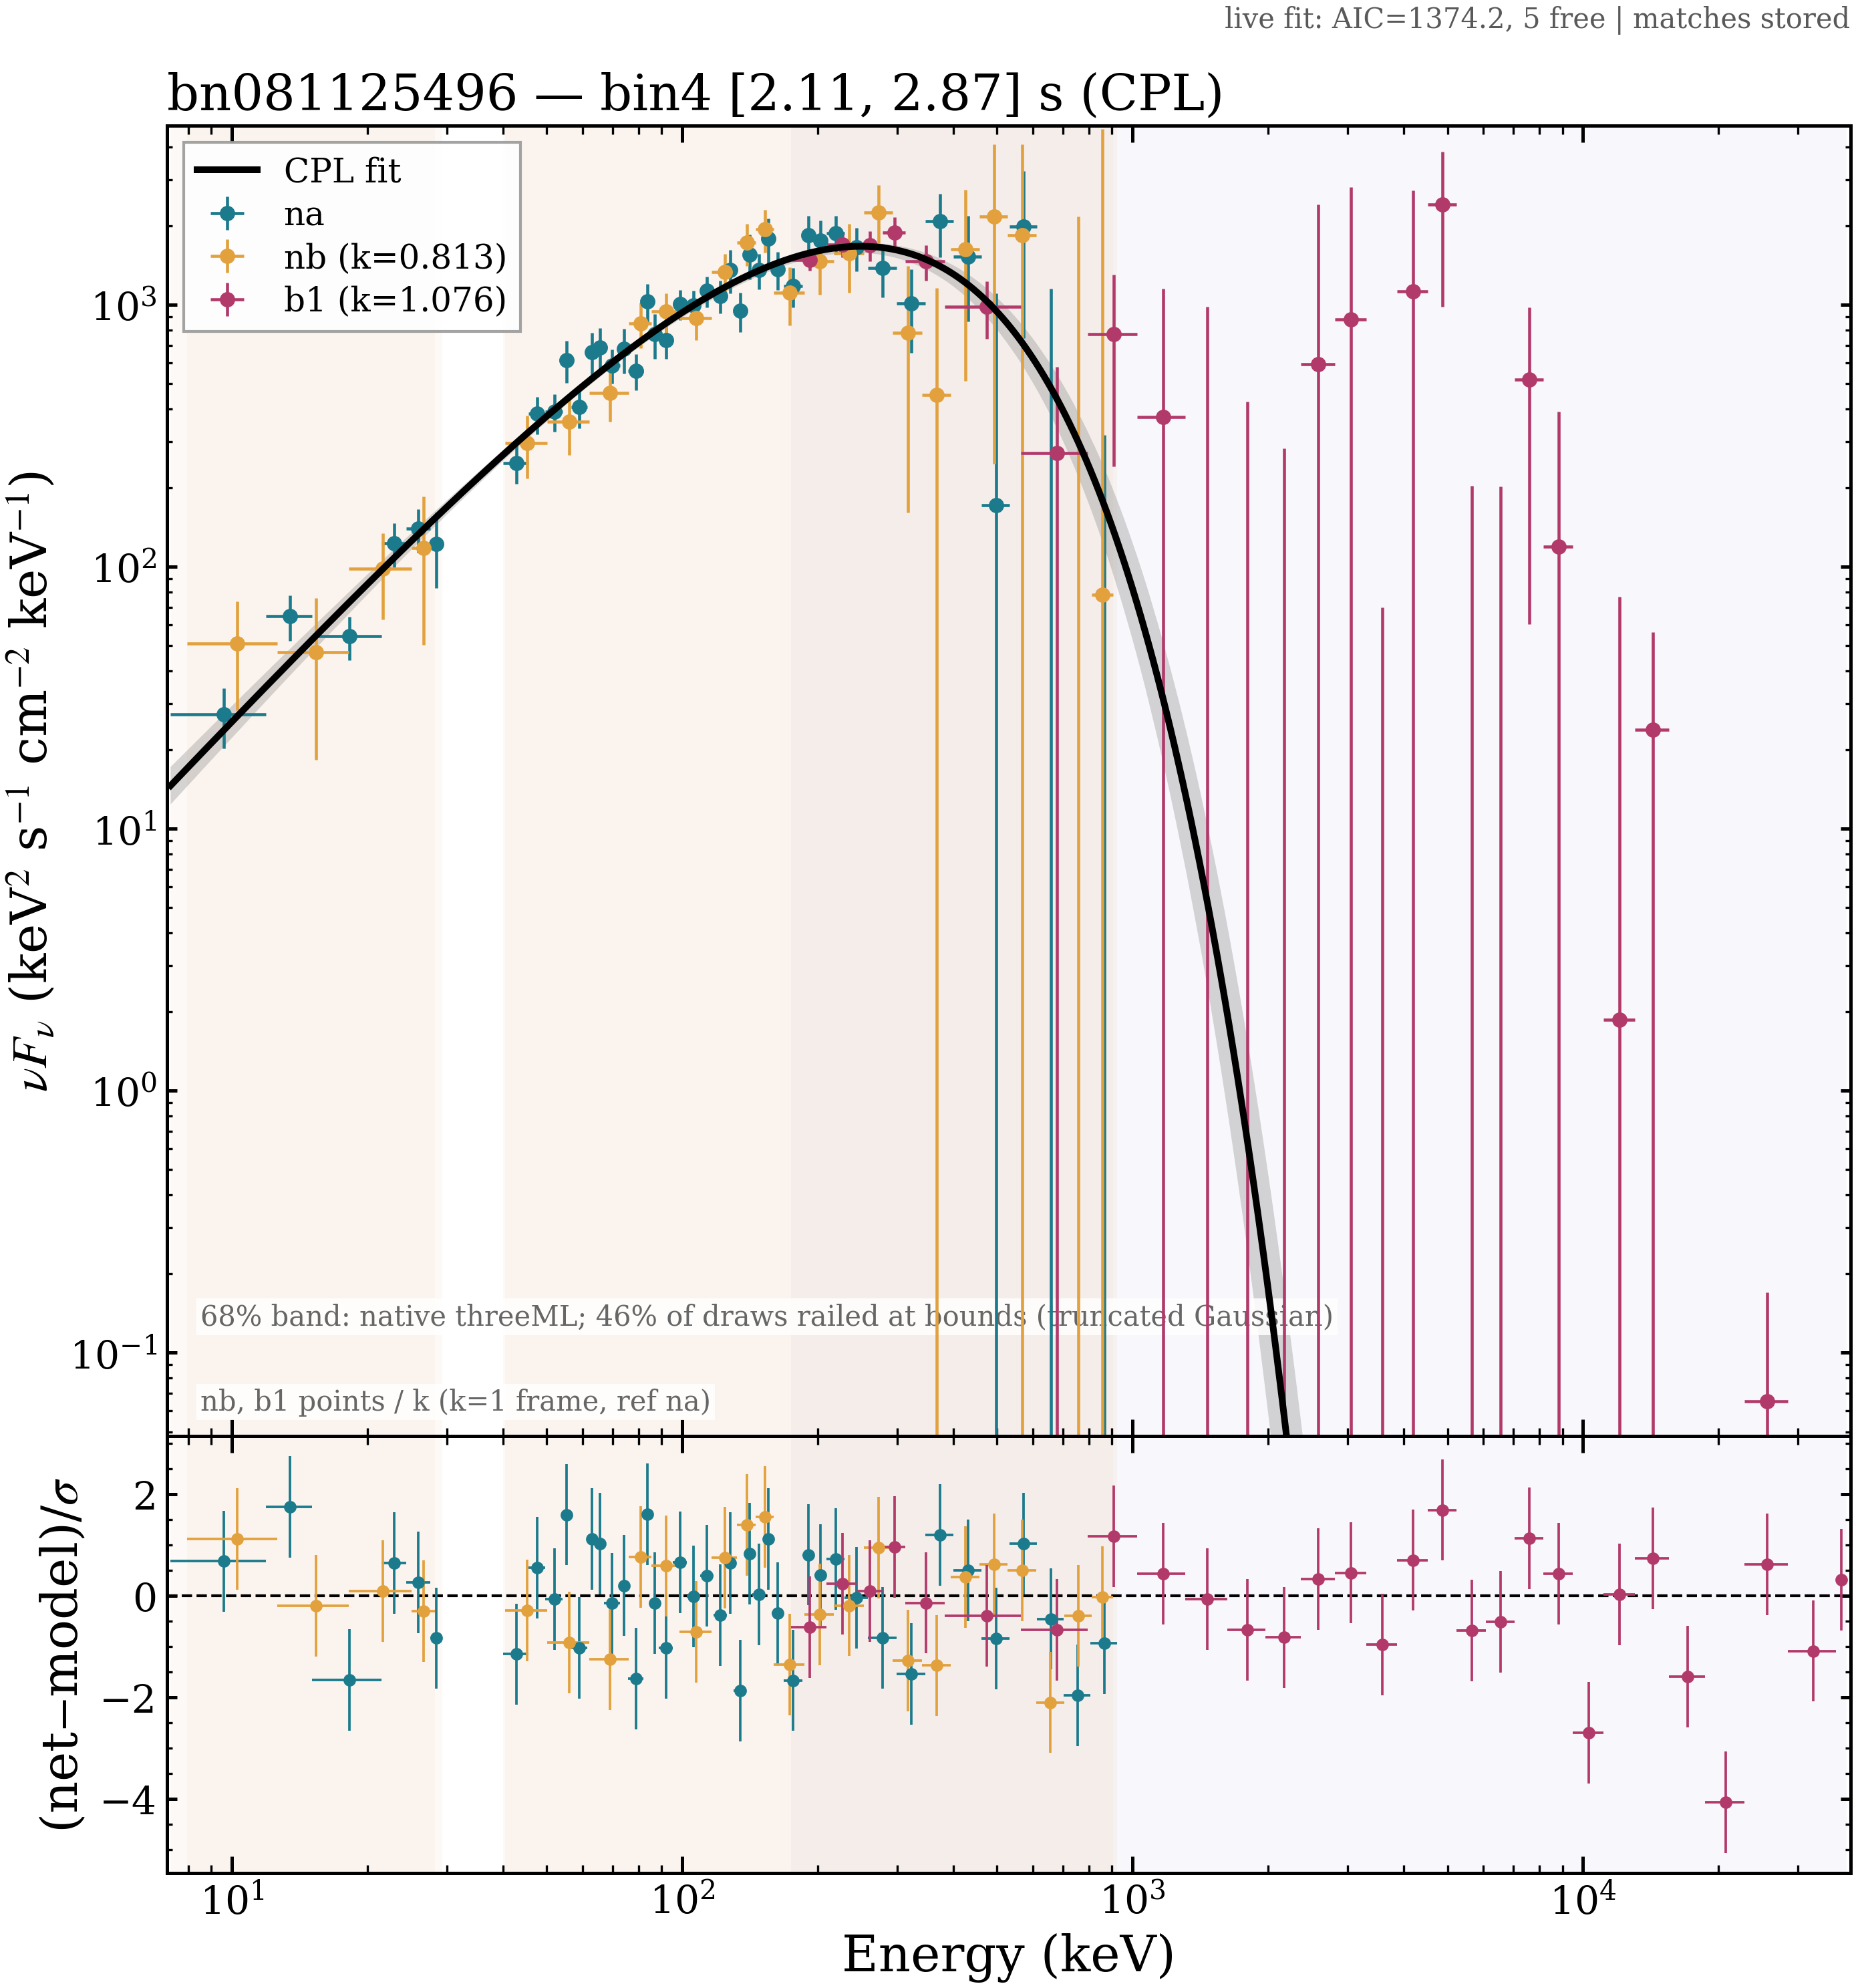
\includegraphics[width=\columnwidth]{figs/bn081125496_SED_bin4_CPL.png}
\caption{Same as Figure~\ref{fig:sedtint} for bin 4 with the winning cutoff
power law. \label{fig:sedbin4}}
\end{figure}

\begin{figure*}
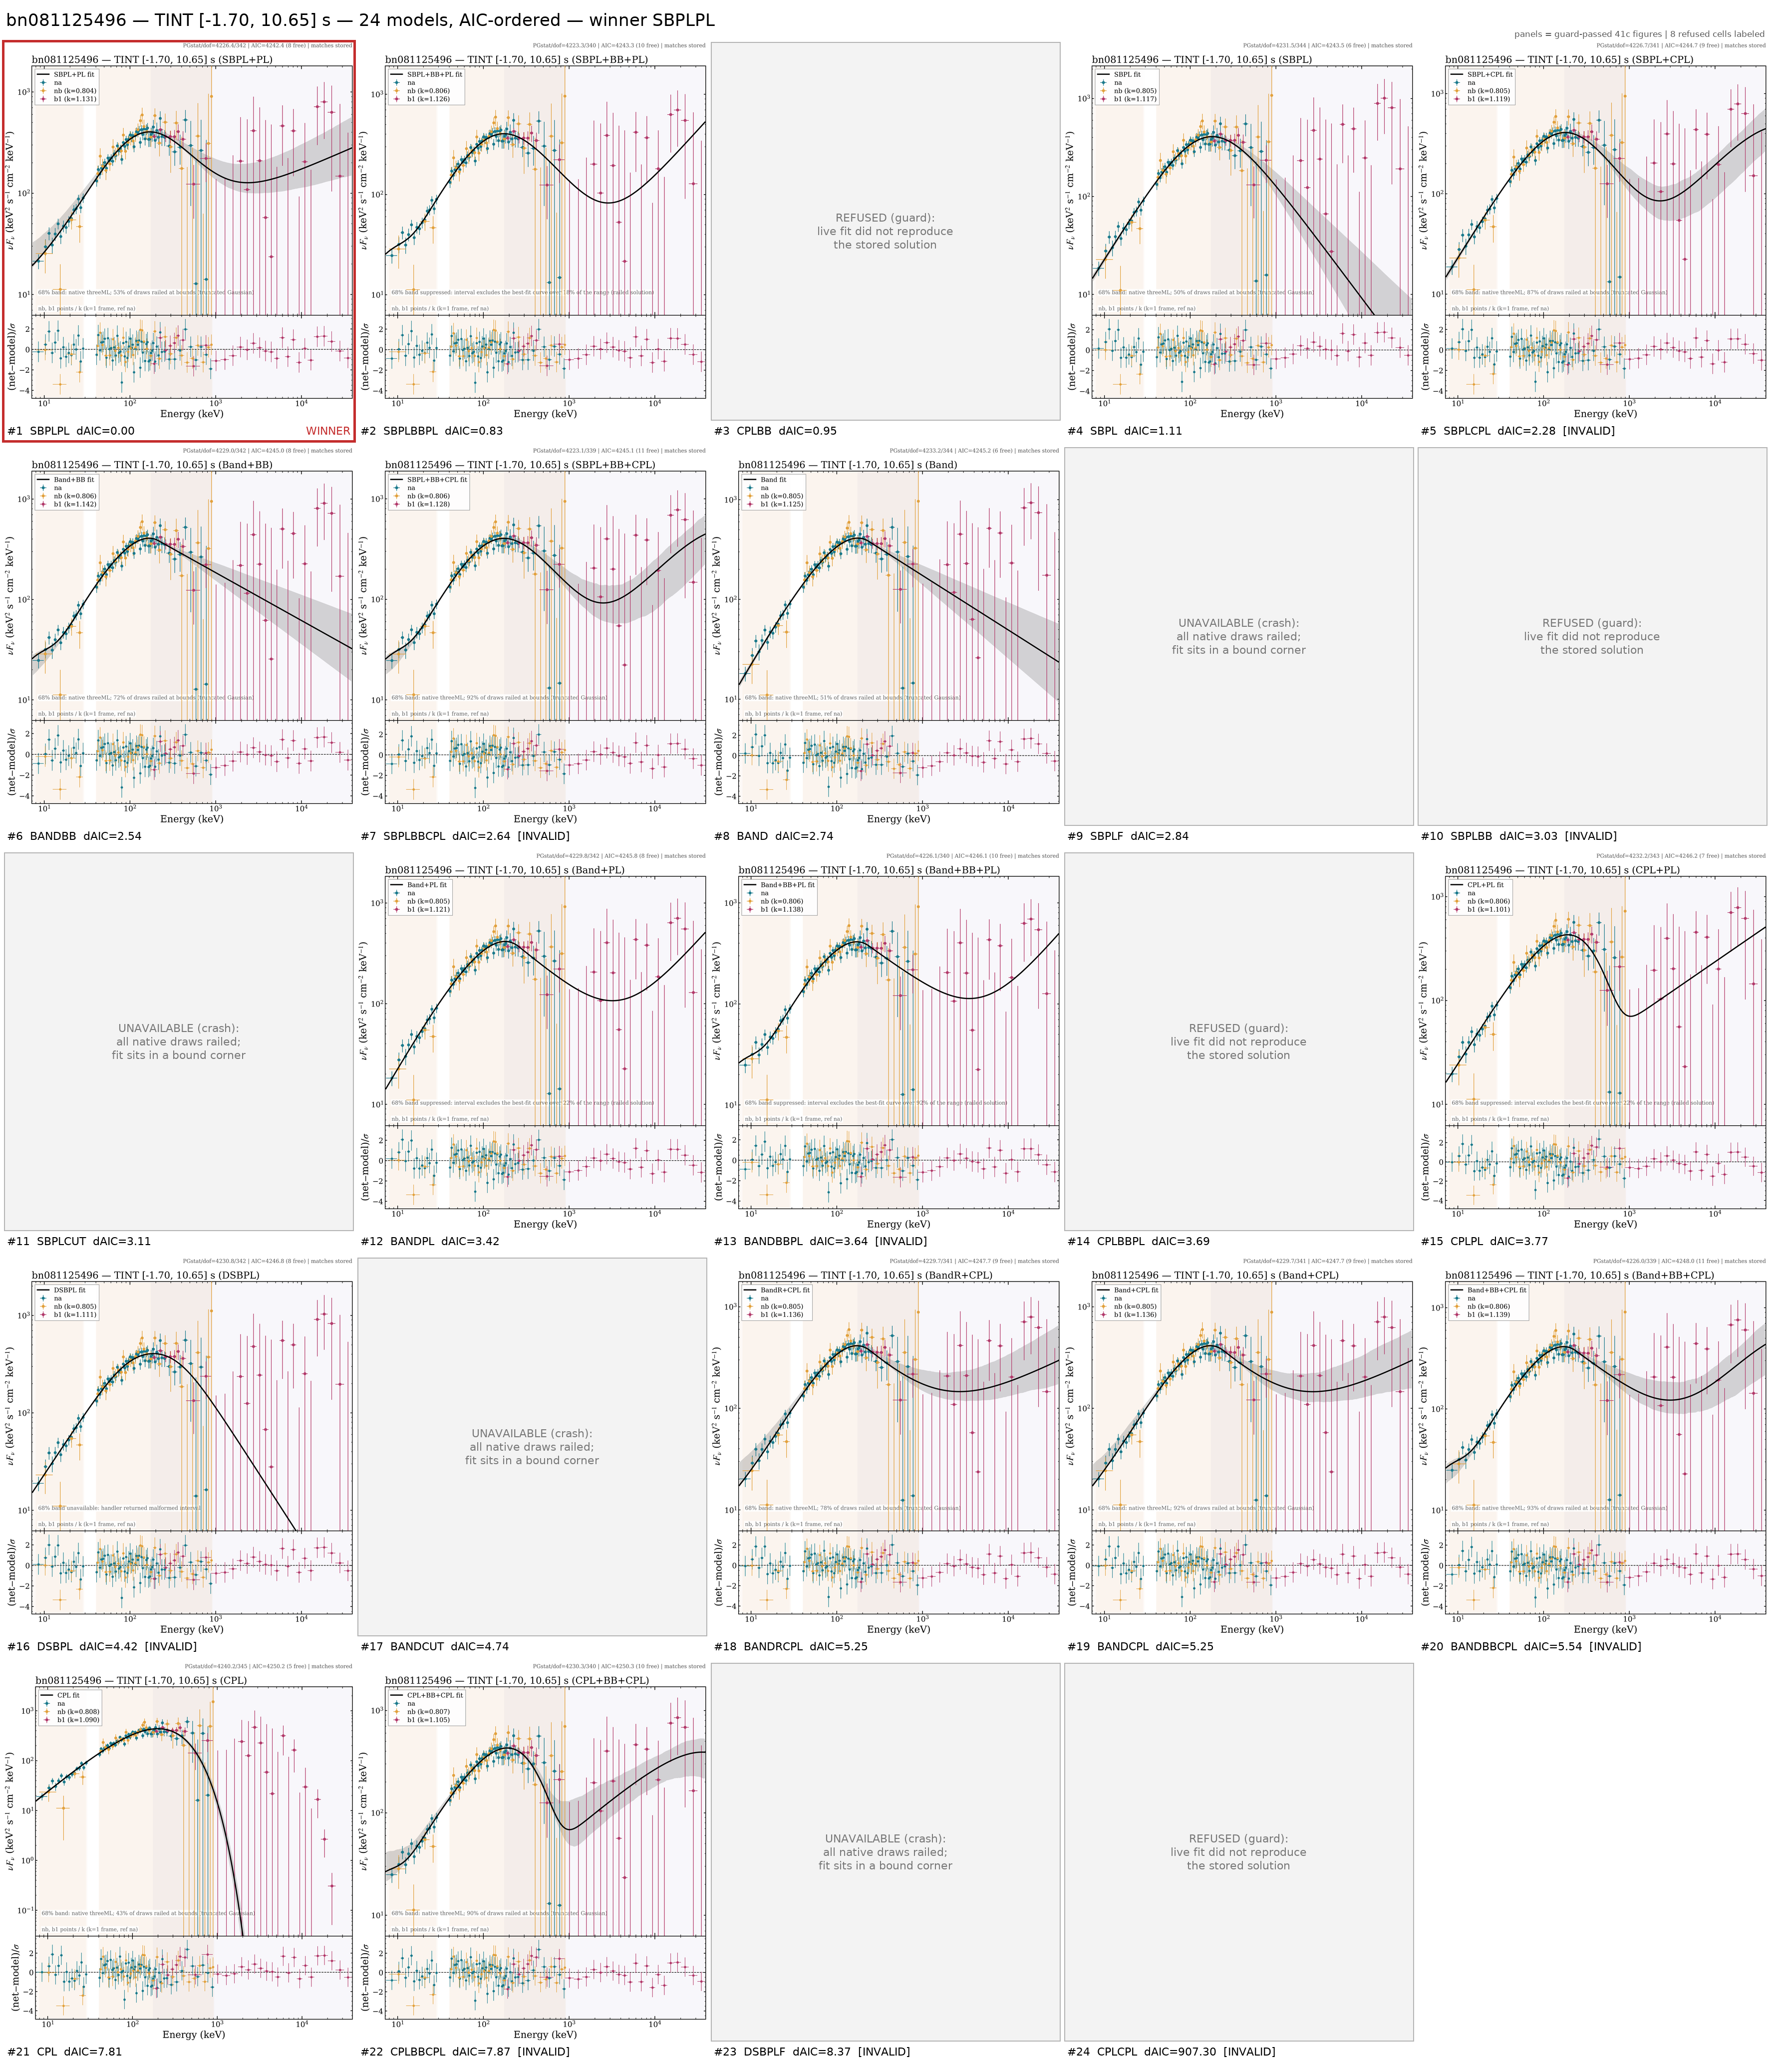
\includegraphics[width=\textwidth]{figs/bn081125496_montage_TINT.png}
\caption{All 24 model fits to the time-integrated spectrum, AIC-ordered
(winner top-left, red frame). Refused panels are labeled with the reason
(live fit did not reproduce the stored solution, or degenerate error
propagation); absence is never silent. Per-bin montages:
Appendix~\ref{app:montages}. \label{fig:montage}}
\end{figure*}

\subsection{Parameter Evolution} \label{sec:evolution}

For every model that wins at least one bin we track its parameters across all
bins (Figures~\ref{fig:evoCPL}--\ref{fig:evoSBPLPL}). The CPL panels carry
the burst's spectral history: the cutoff energy declines from
$\simeq 320$~keV on the rise to $\simeq 59$~keV in the late decay --- hard-to-soft
evolution across a factor $\sim$5.5 --- while the low-energy index stays in a
narrow range around $\Gamma \simeq -0.3$, well inside the synchrotron
fast-cooling death line and consistent with marginally fast cooling at the
peak bins. The Band panels show $\beta$ railing to $-5$ (a CPL clone)
everywhere except where the tail is real (bins 2, 5, 8). The SBPL+PL panel
makes \S\ref{sec:specresults}'s point graphically: the model is valid in one
bin only.

\begin{figure}
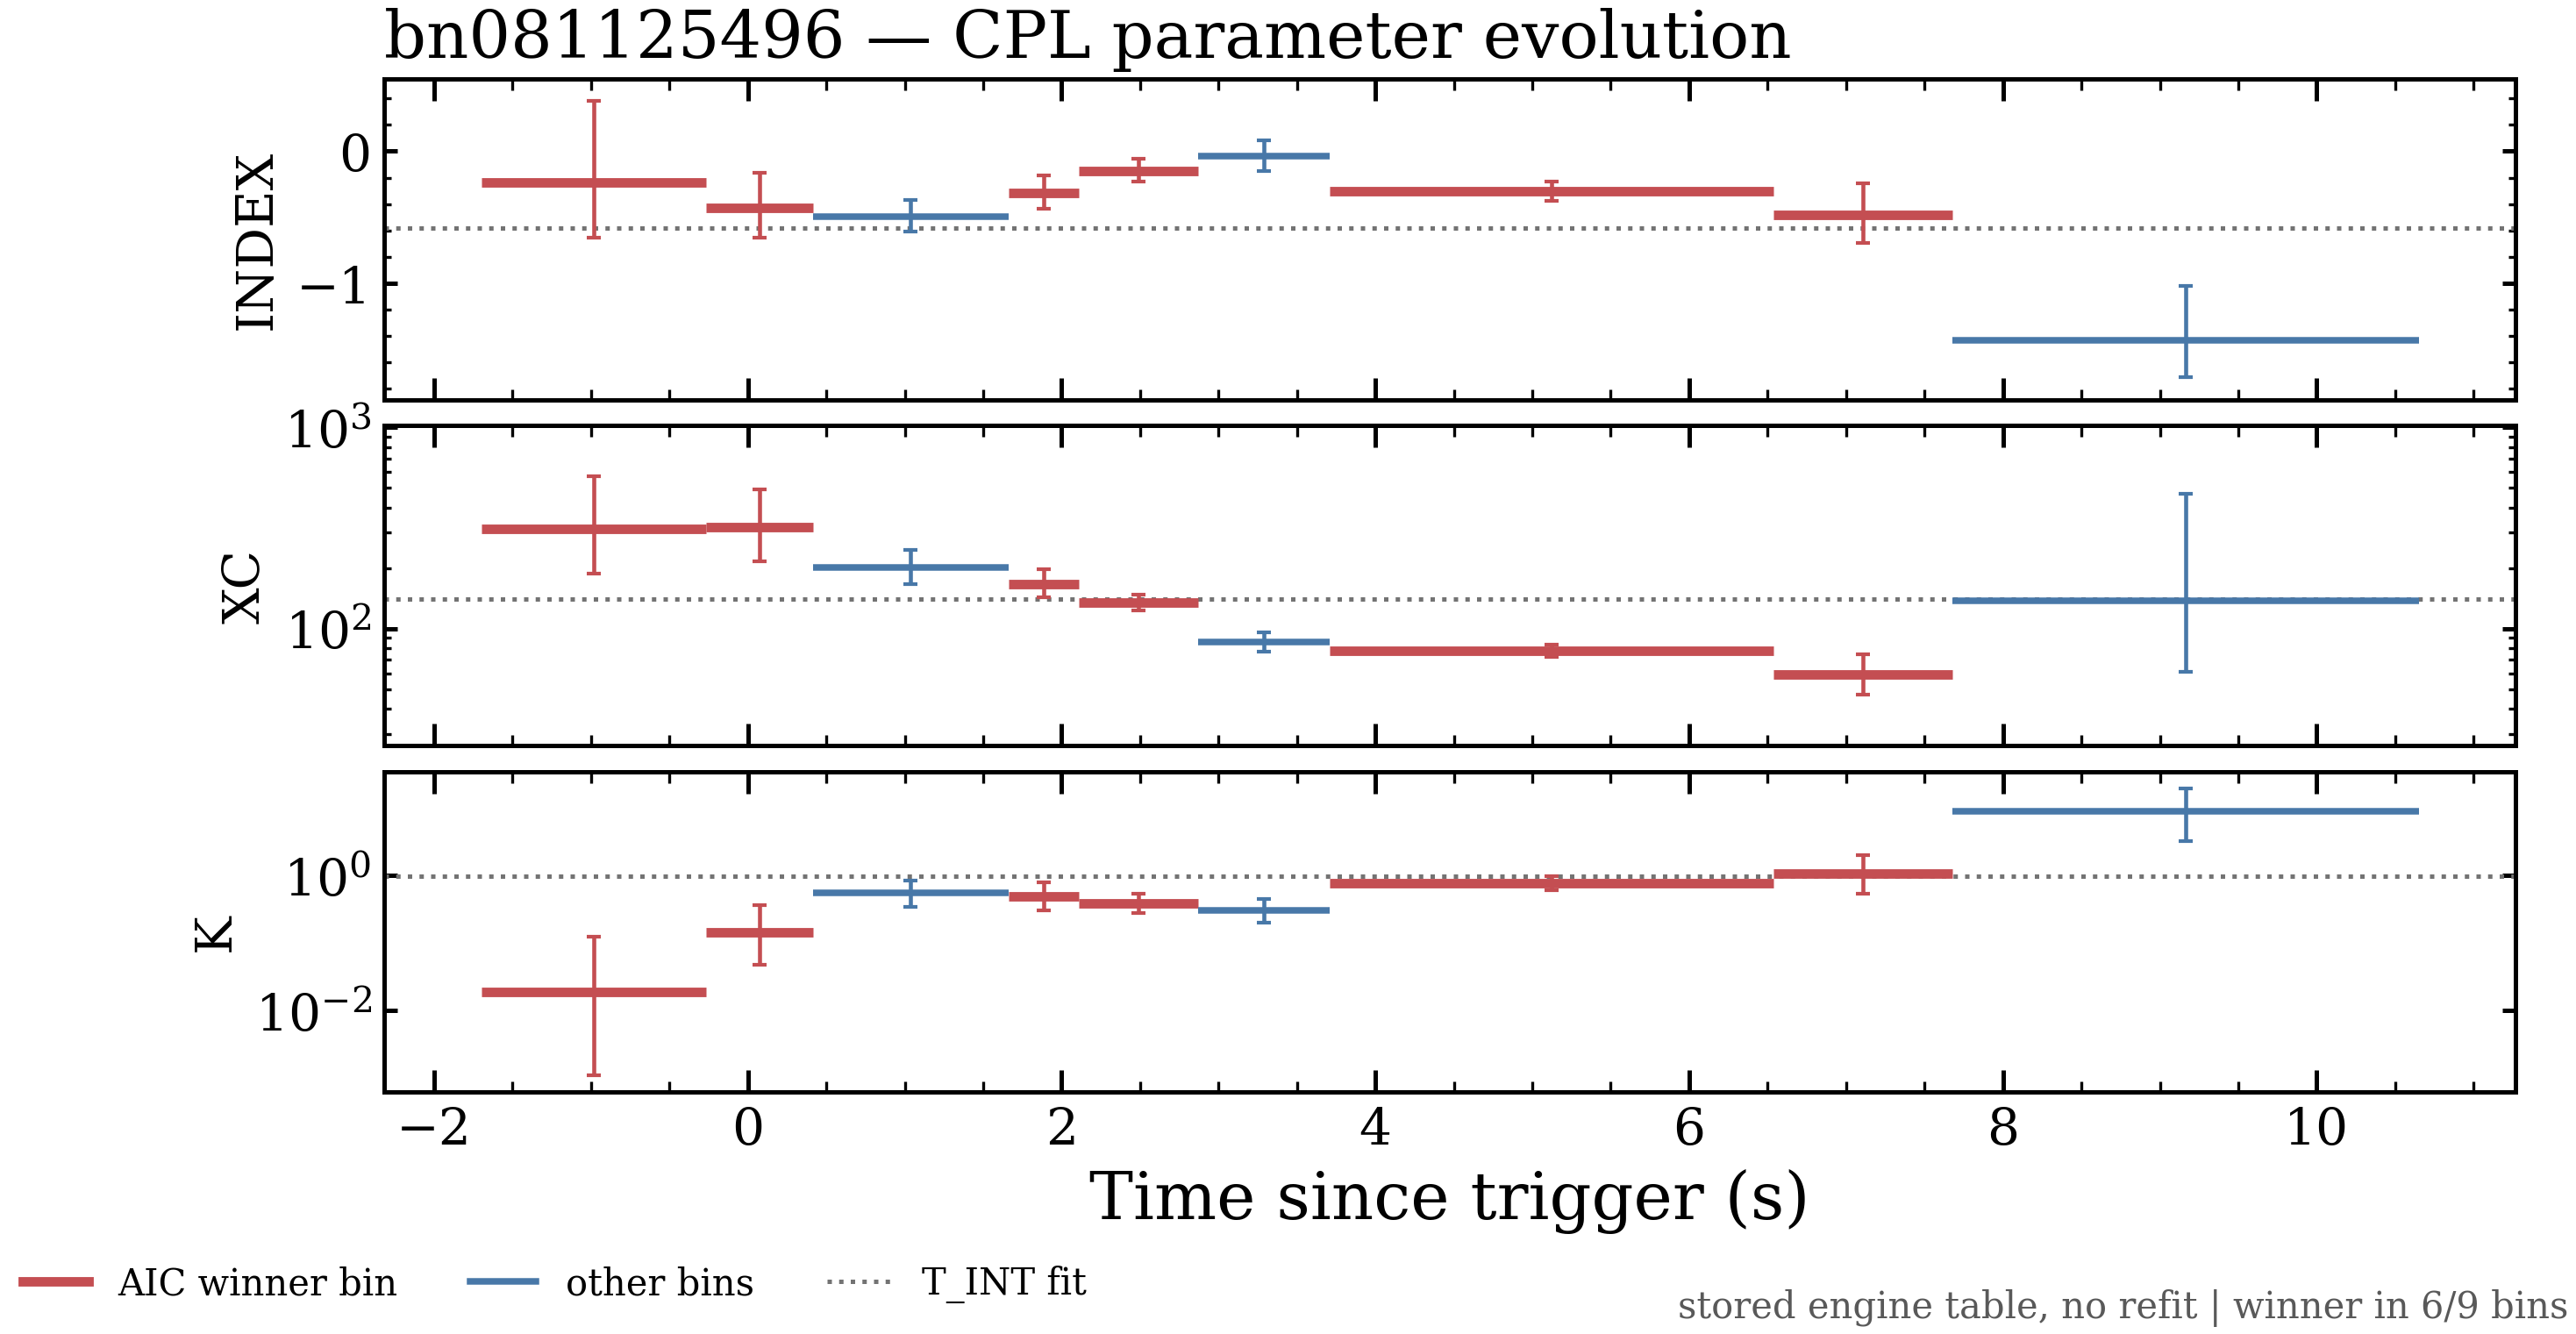
\includegraphics[width=\columnwidth]{figs/bn081125496_paramevo_CPL.png}
\caption{CPL parameter evolution across the nine bins. Top to bottom:
low-energy index $\Gamma$, cutoff energy $E_{\rm c}$, and normalization.
Horizontal bars span each time bin; red bars mark bins where CPL is the AIC
winner; the dotted line is the time-integrated value. $E_{\rm c}$ carries the
burst's hard-to-soft history while $\Gamma$ stays near $-0.3$.
\label{fig:evoCPL}}
\end{figure}

\begin{figure}
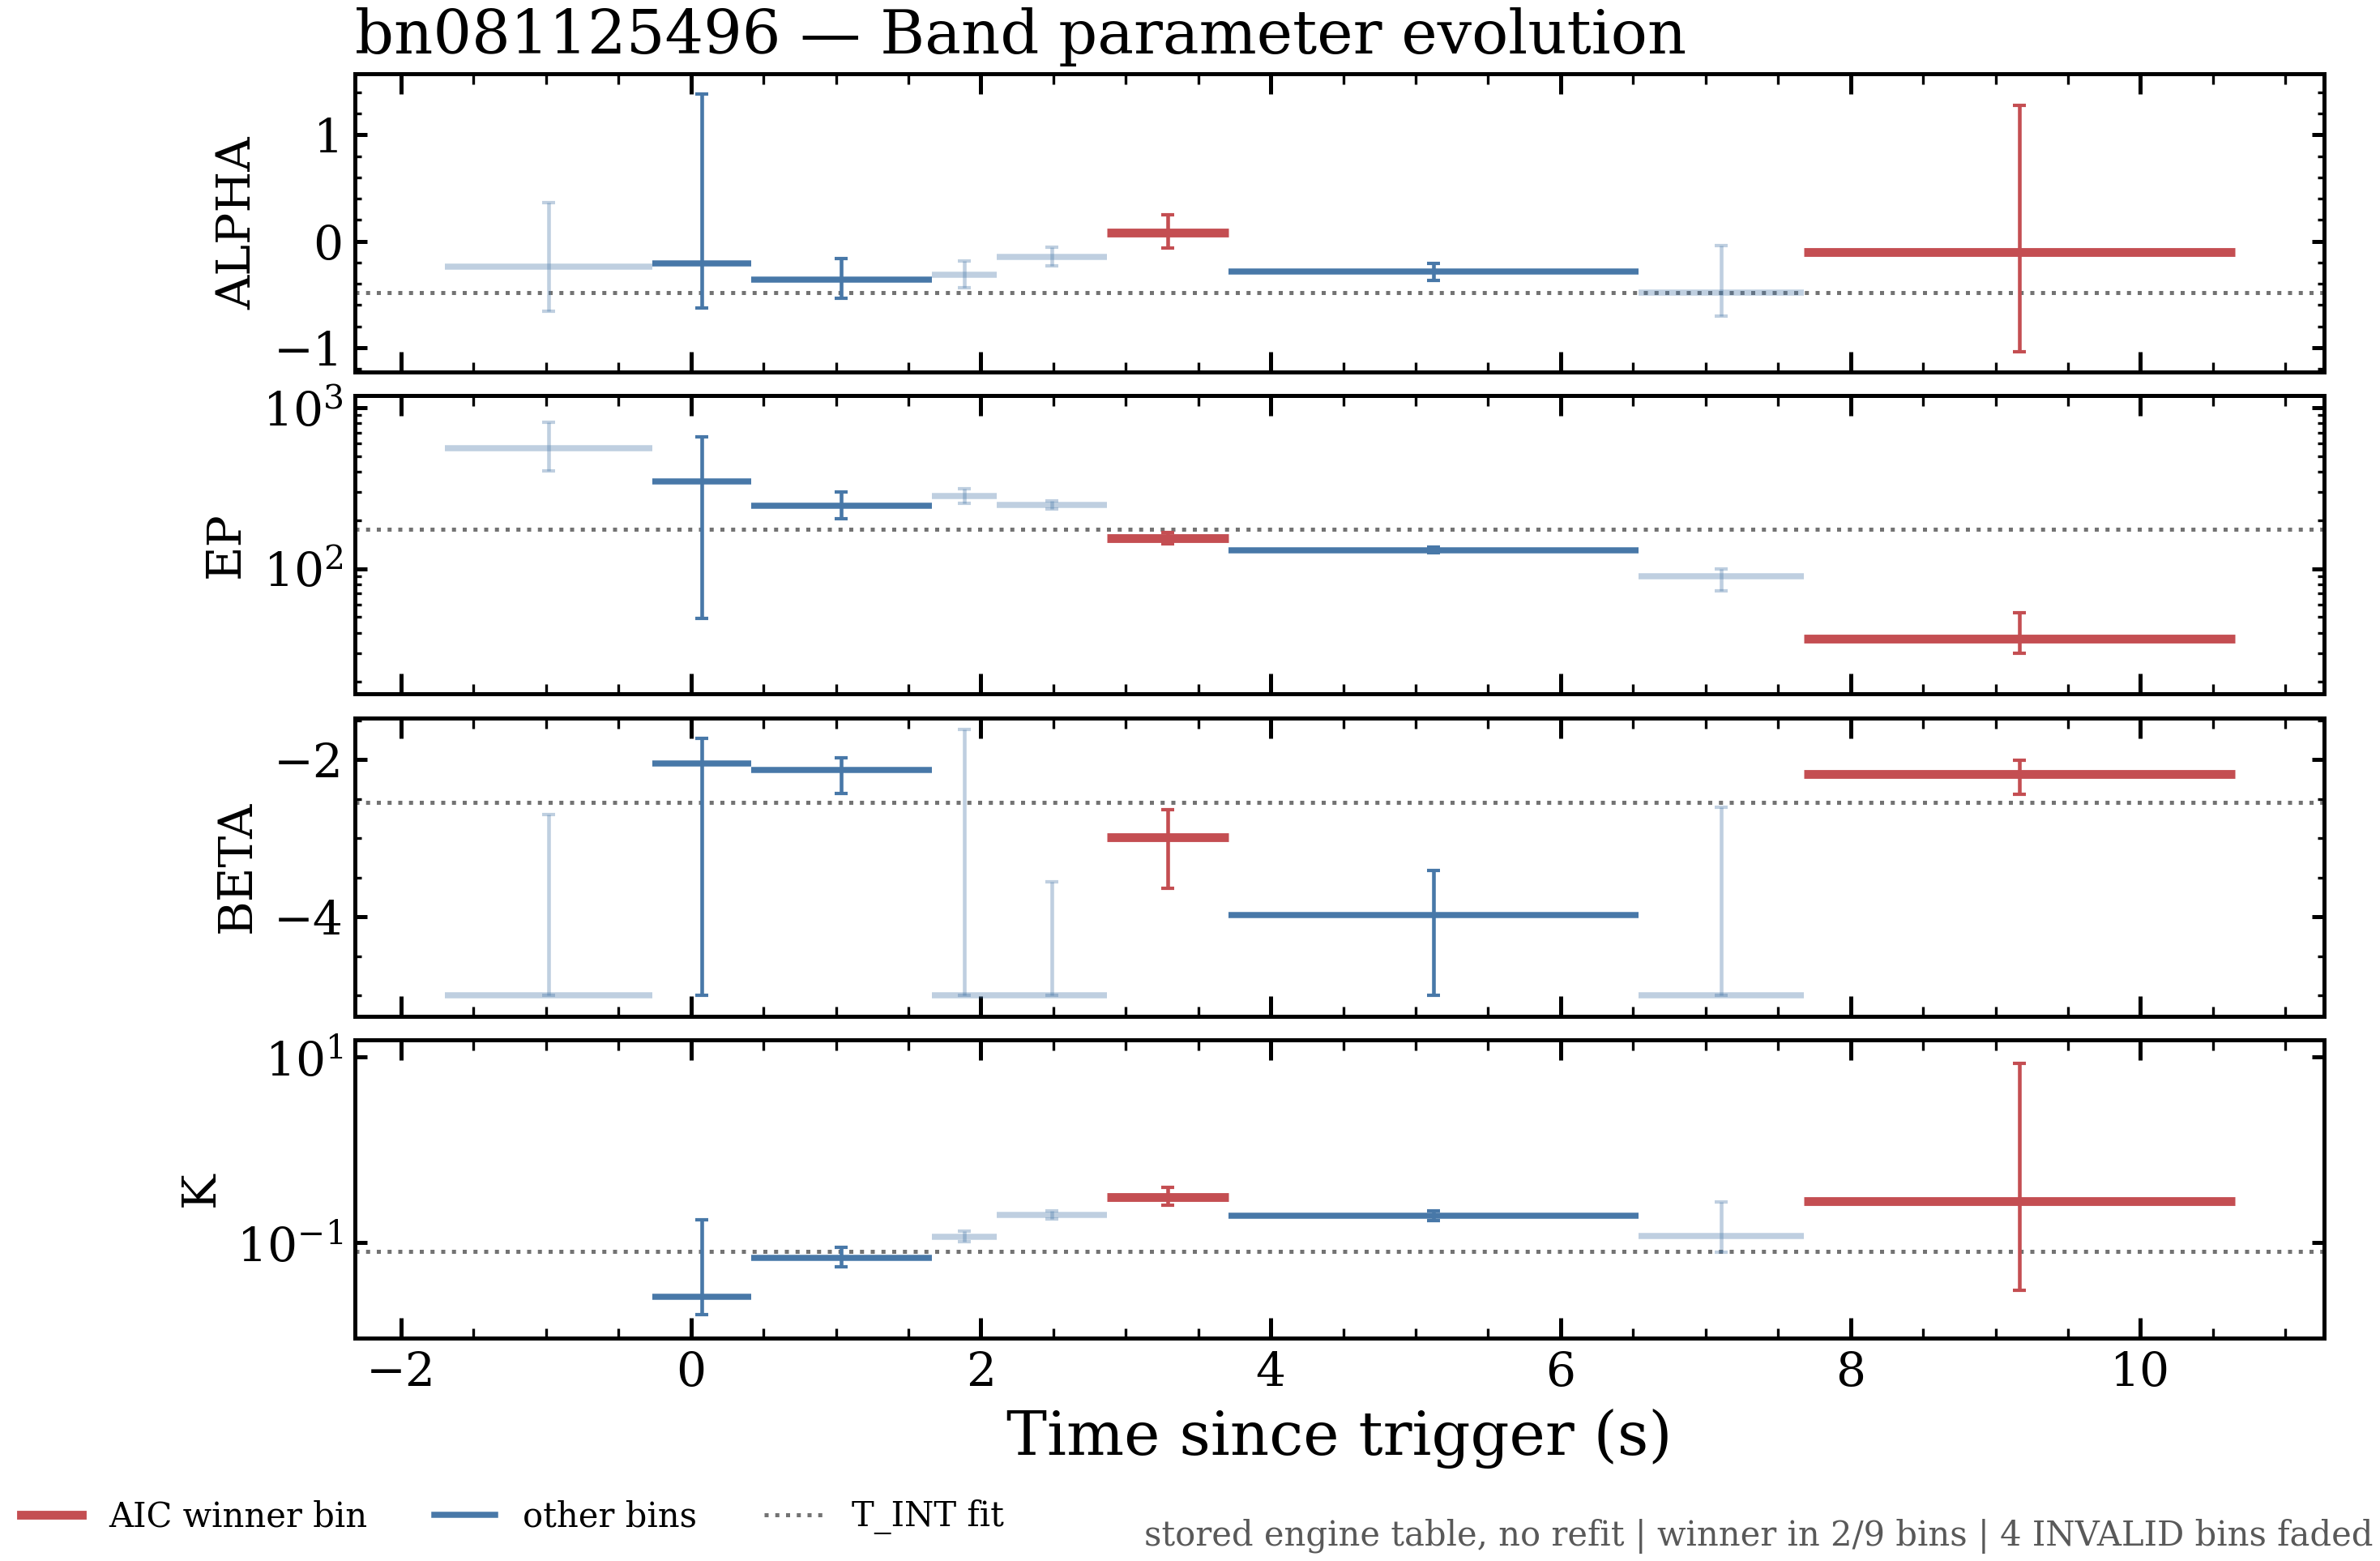
\includegraphics[width=\columnwidth]{figs/bn081125496_paramevo_BAND.png}
\caption{As Figure~\ref{fig:evoCPL} for the Band function. Faded bars are
fits failing validity gates (railed parameters). \label{fig:evoBAND}}
\end{figure}

\begin{figure}
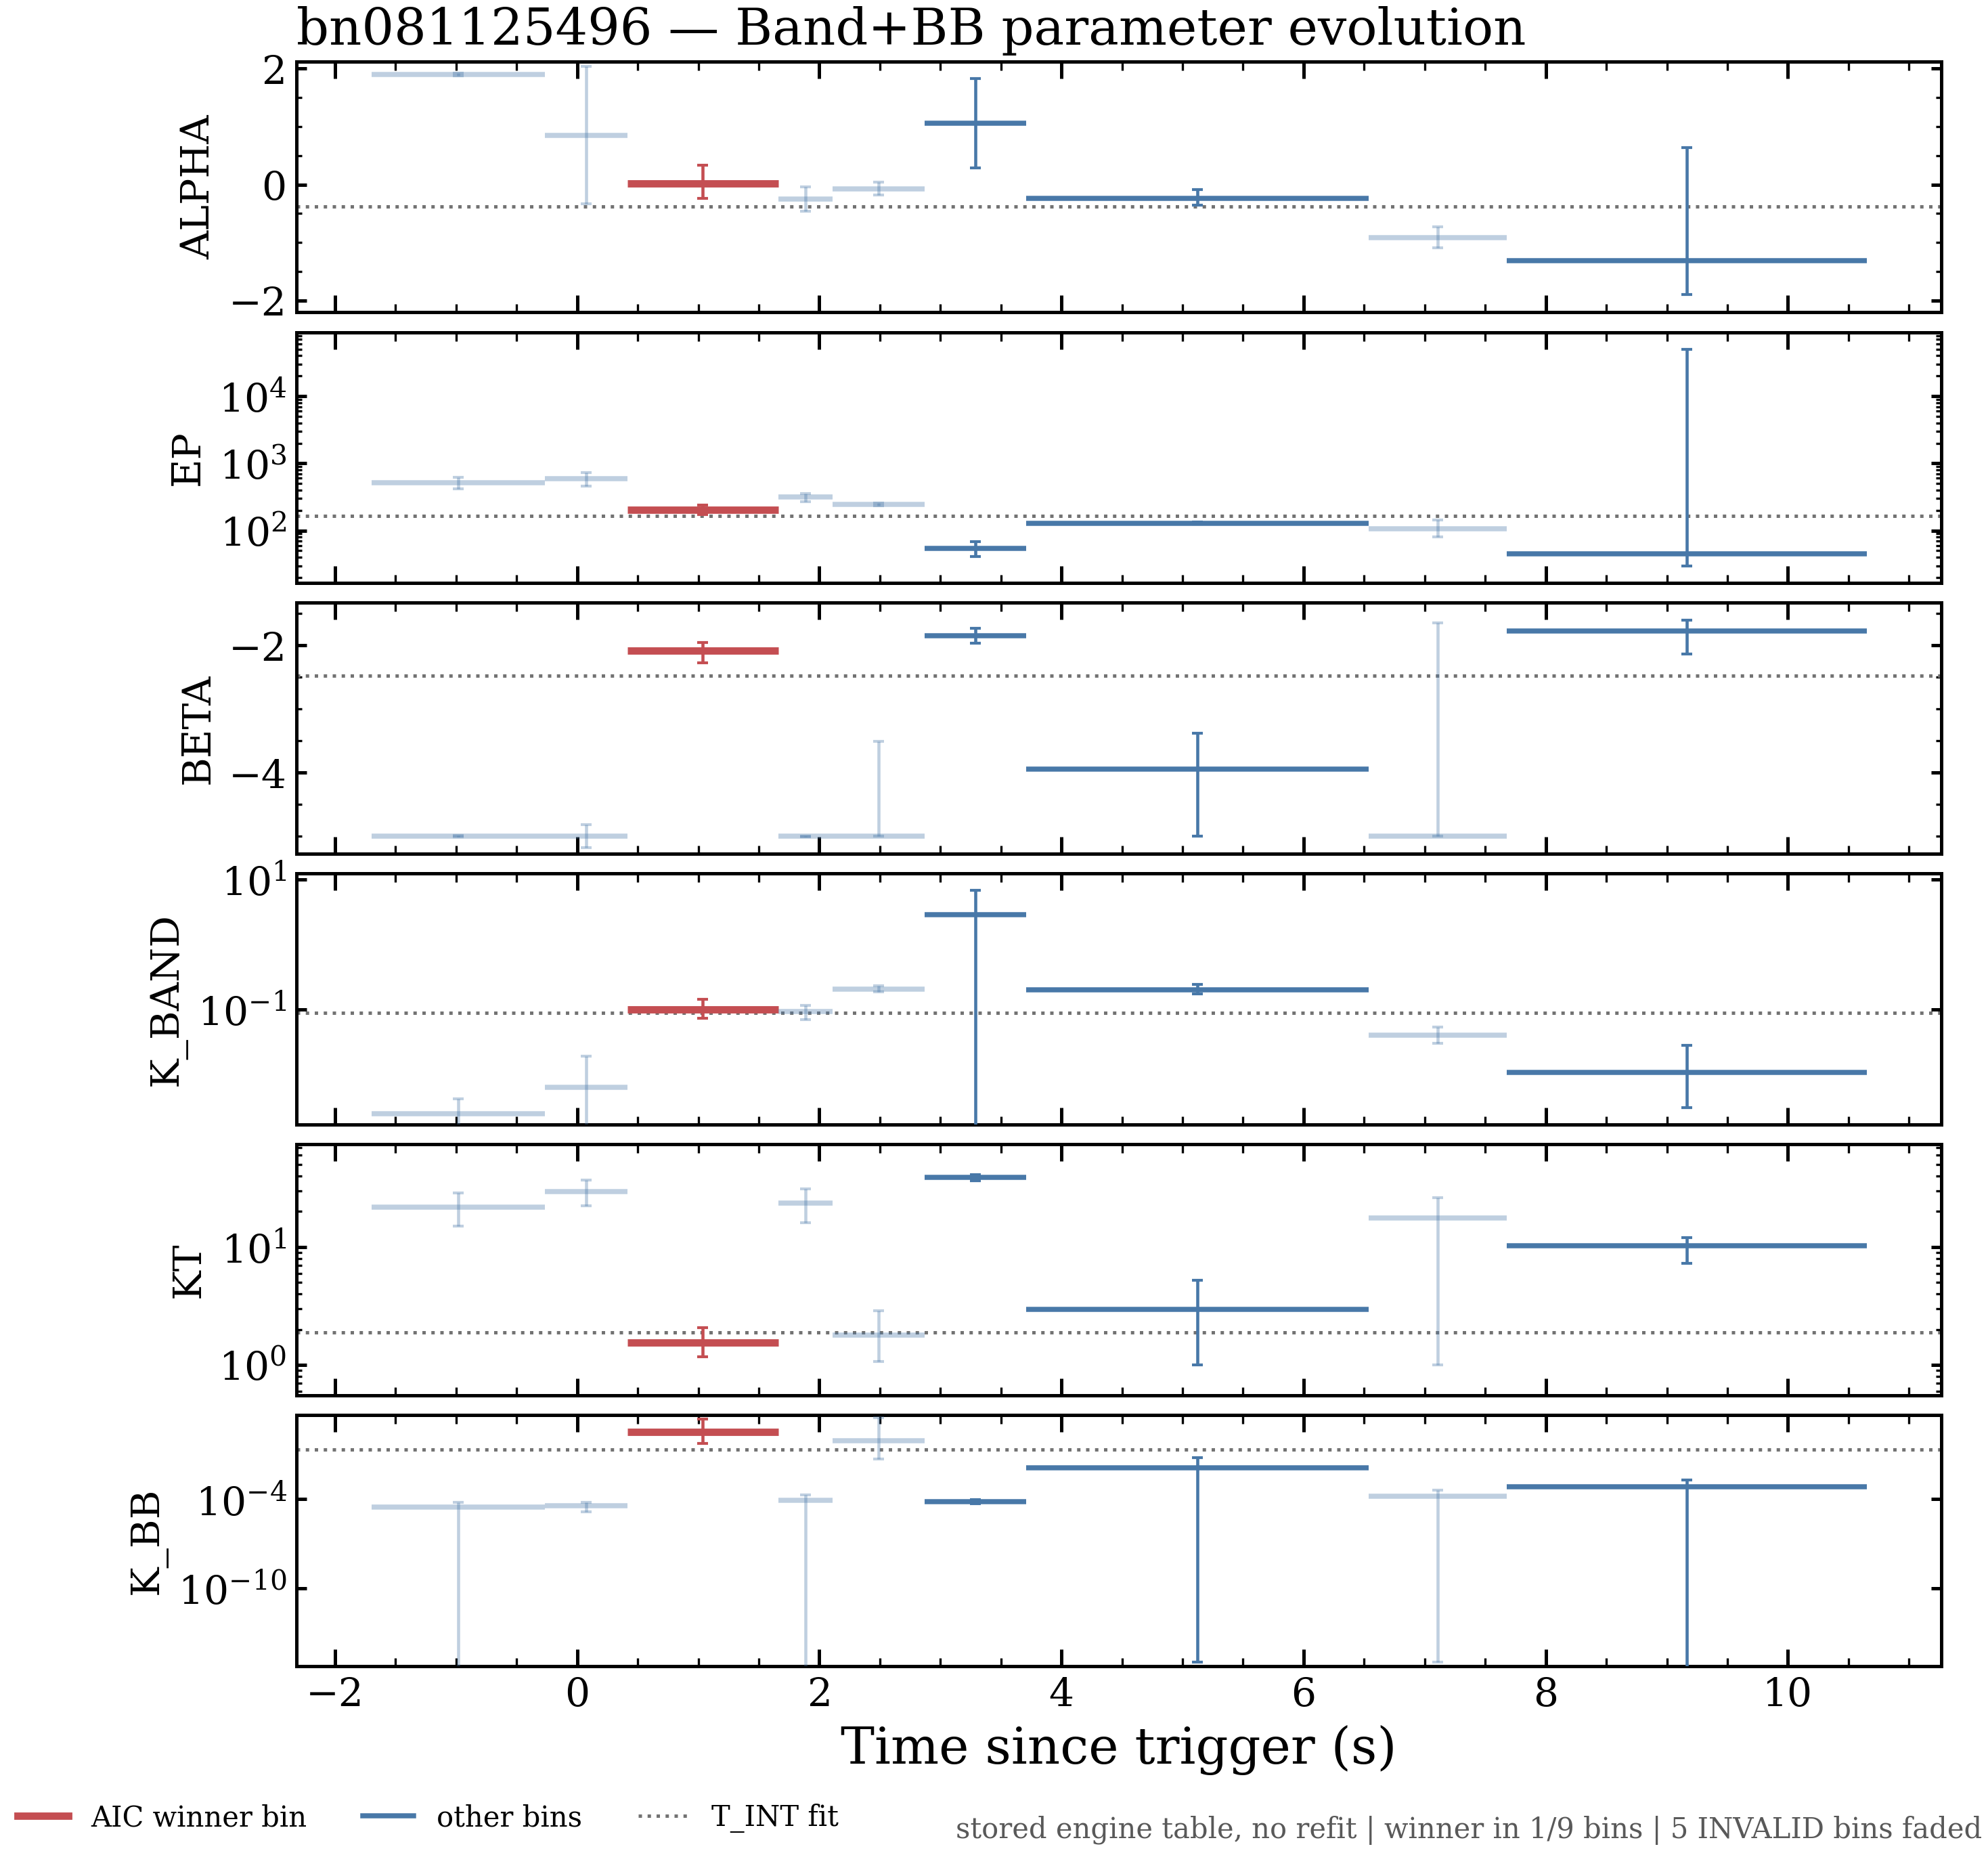
\includegraphics[width=\columnwidth]{figs/bn081125496_paramevo_BANDBB.png}
\caption{As Figure~\ref{fig:evoCPL} for Band+BB. The $kT$ panel shows the
edge-constrained cluster near 1.5~keV (\S\ref{sec:specresults}).
\label{fig:evoBANDBB}}
\end{figure}

\begin{figure}
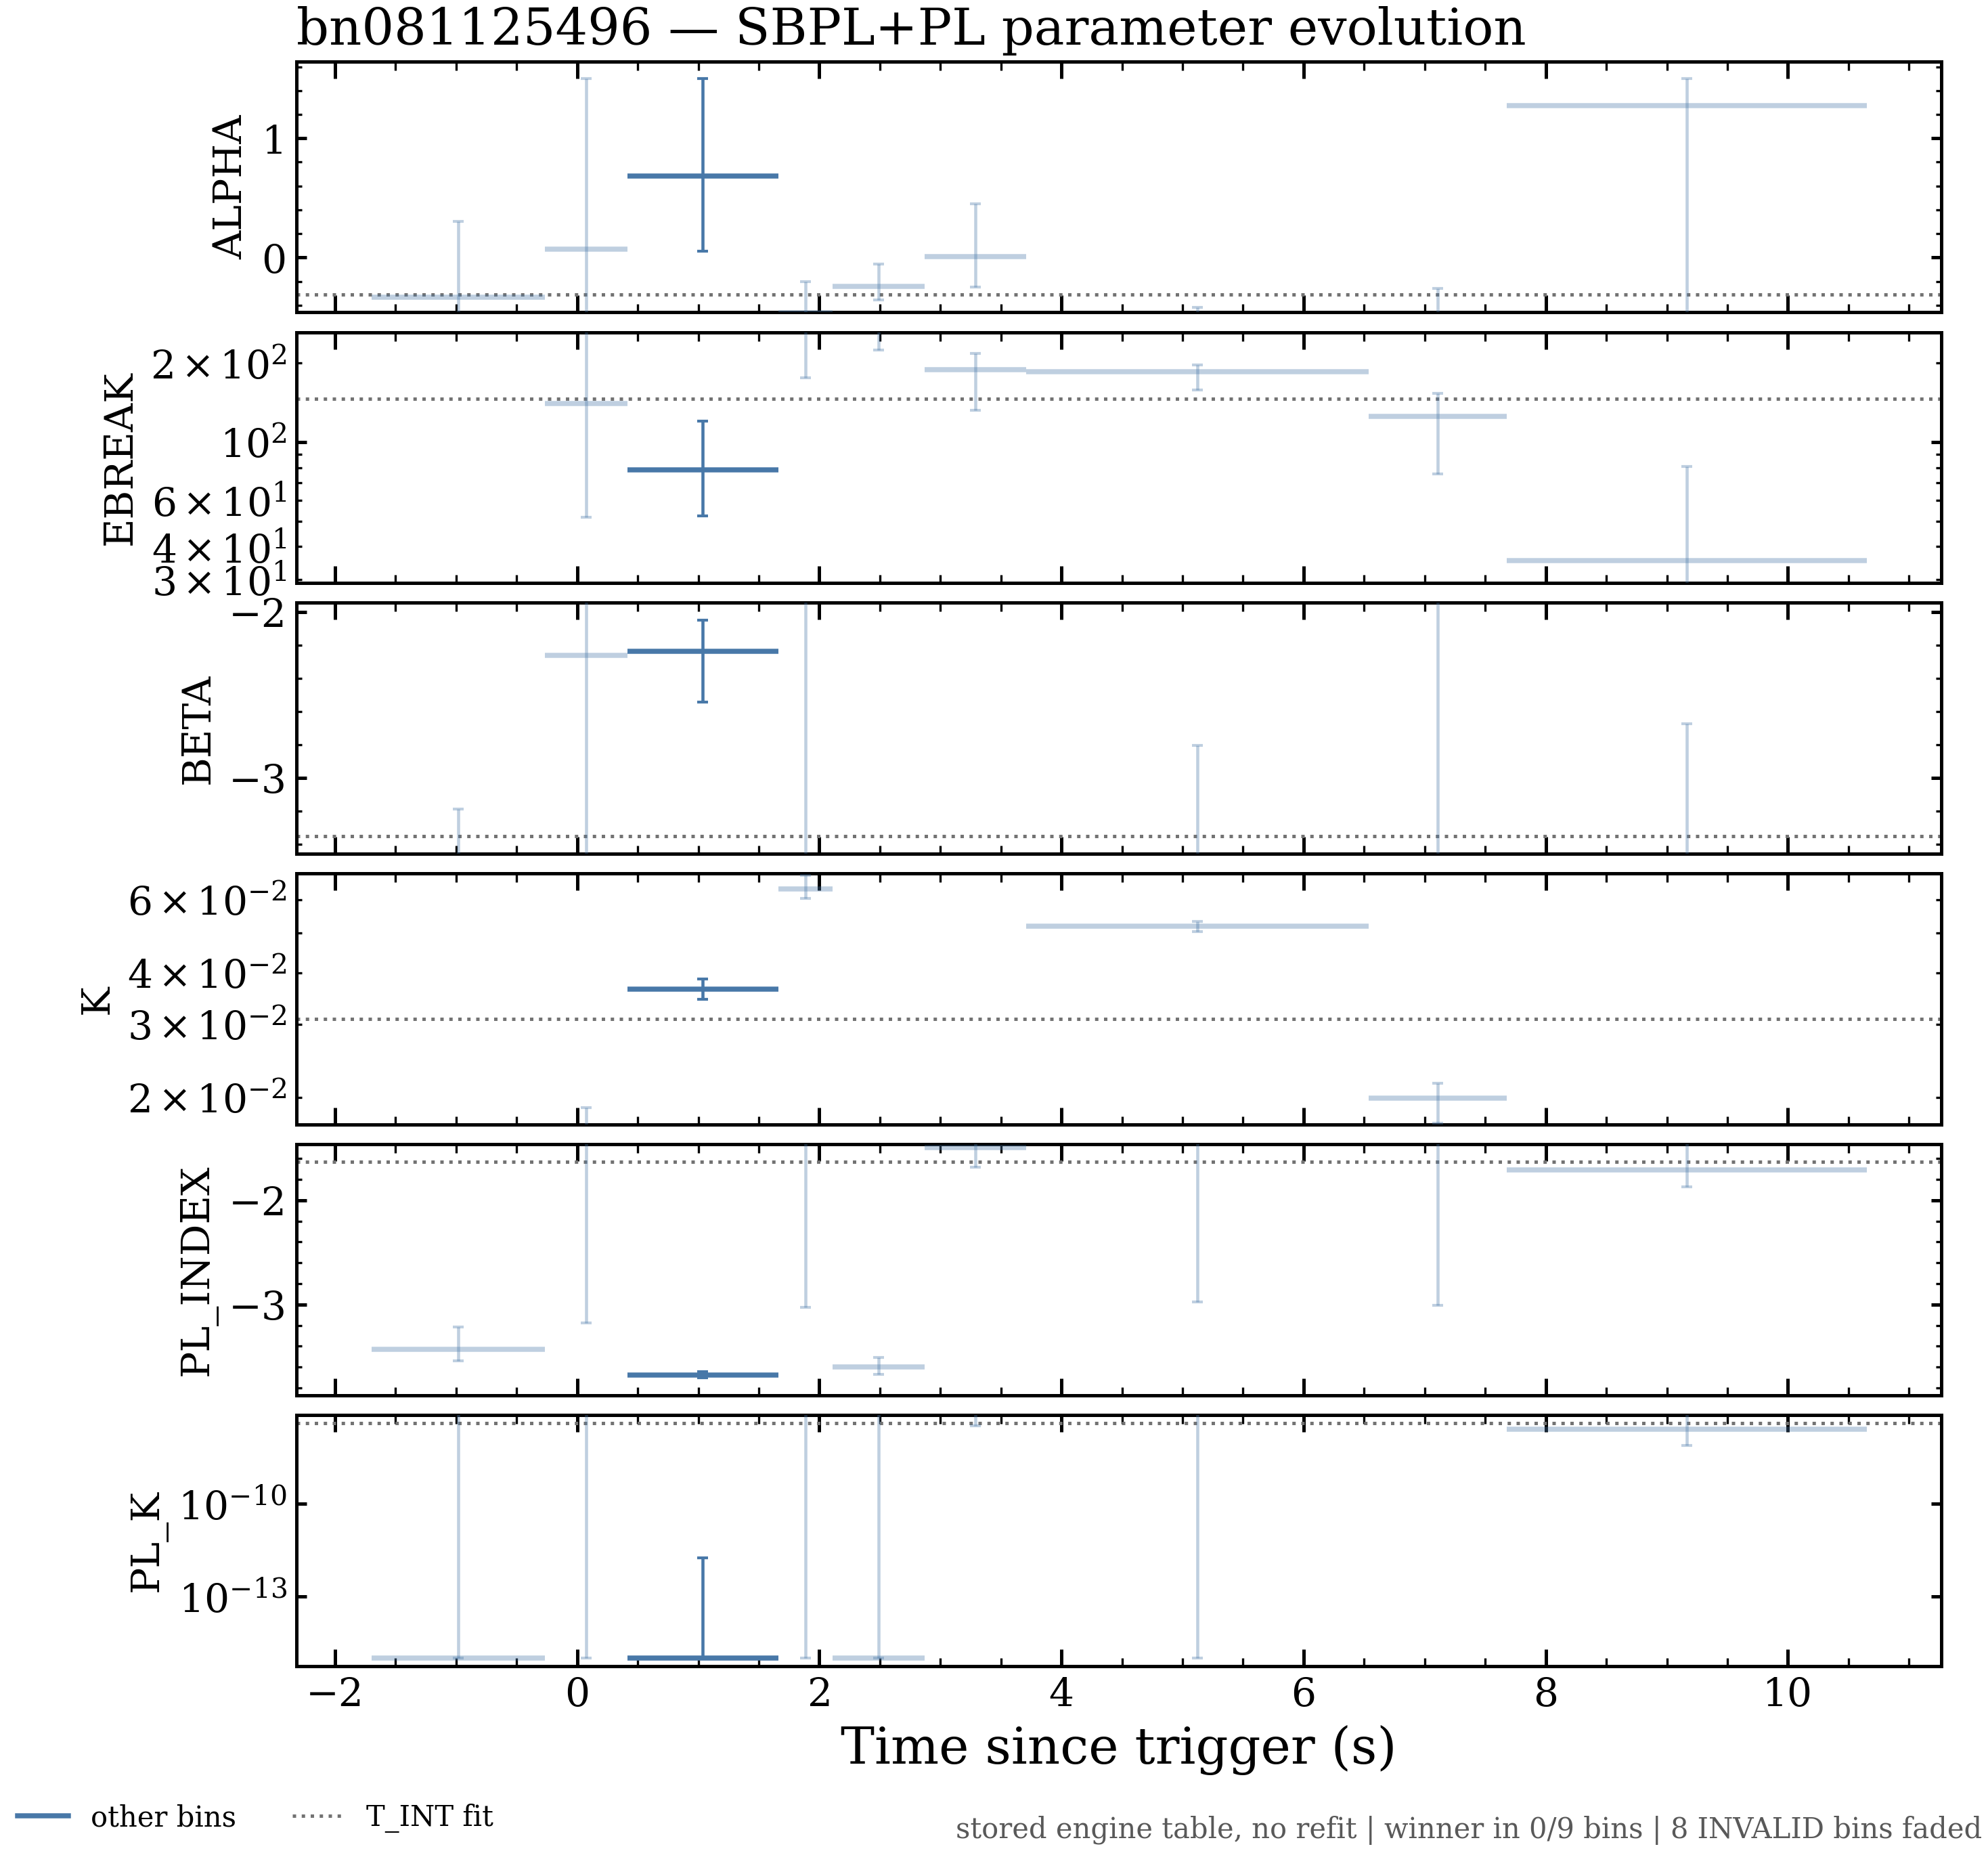
\includegraphics[width=\columnwidth]{figs/bn081125496_paramevo_SBPLPL.png}
\caption{As Figure~\ref{fig:evoCPL} for SBPL+PL, the time-integrated winner:
valid in a single resolved bin. \label{fig:evoSBPLPL}}
\end{figure}

\section{Discussion} \label{sec:discussion}

Assembled, the burst reads as one coherent object:

\textbf{One pulse, one continuum, evolving.} A cutoff power law with
$\Gamma \simeq -0.3$ and a decaying $E_{\rm c}$ describes seven of nine bins;
the hard tail appears exactly where fast evolution concentrates photons above
the cutoff (the rise) and where the decaying $E_{\rm p}$ drags the band
window onto the tail (the late bins). The time-integrated composite winner is
the integral of this evolution, not an extra emission component --- a
single-burst caution for integrated-spectrum component claims
\citep[cf.][]{2019ApJ...886...20Y}.

\textbf{No photosphere, and a reusable artifact class.} The blackbody census
is null, and its failure mode is instructive: every ``significant'' low-$kT$
solution is pinned below the fitted band's edge. A simple gate --- flag any
thermal component whose Wien peak falls below the fitted range --- removes
the entire class and will be applied across the campaign.

\textbf{Timing quantities are estimator statements.} The same data return
MVTs of 34, 215, and 546~ms under three published estimators, and a lag that
is best read as $8\%$ of the pulse width. None of these is wrong; each
answers its own question. For population work --- lag--luminosity
\citep{2012MNRAS.419..614U}, lag--MVT curvature tests
\citep{2013ApJ...778....3S,2025JARNA..11...27G}, MVT compactness limits ---
the estimator, band, frame, and window must travel with every number, and
single-pulse samples are where those choices can be controlled.

\section{Analysis Provenance} \label{sec:provenance}

Every figure in this paper passed a fresh-context verification gate
(producer--verifier separation) before inclusion; every fitted value is bound
to a machine-readable provenance sidecar (inputs, seeds, likelihood values,
software hashes); live fits are hard-guarded to reproduce stored solutions to
$|\Delta\mathrm{AIC}| < 0.1$; and refused or degenerate fits are enumerated
with reasons rather than omitted. The complete gate ledger and per-bin
reviewer notes are archived with the campaign products. A companion paper
describes the agentic pipeline and its verification architecture.

\section{Summary} \label{sec:summary}

We analyzed \grb\ end-to-end with the single-pulse campaign pipeline:
\begin{enumerate}
\item $T_{90} = 8.50^{+0.15}_{-0.19}$~s (windowed lower limit;
$5.3\sigma$ tail beyond the window), $T_{90} \propto E^{-0.14\pm0.02}$,
FRED-like asymmetry $\varphi = 0.317 \pm 0.026$ (Kocevski profile best).
\item MVT $= 33.9 \pm 2.9$~ms (windowed, on the pulse rise; $z = 2.5$
caveat), versus 215~ms (global CWT) and 546~ms (global Haar) --- estimator
labels are part of the measurement.
\item Lag $= 0.705^{+0.291}_{-0.205}$~s (soft lags hard) $\approx 8\%$ of the
pulse width: envelope evolution, with direct implications for population
lag--variability correlations.
\item CPL suffices in 7/9 bins ($\Gamma \simeq -0.3$, $E_{\rm c}$ declining
$321 \rightarrow 59$~keV); a hard tail ($\beta \simeq -2.1$) is demanded only
on the pulse rise and in the late tail.
\item The time-integrated winner (SBPL+PL) wins no resolved bin ---
integrated composite components can be spectral evolution in disguise.
\item Zero photospheric evidence in $\sim$90 blackbody-added fits; all
low-$kT$ solutions are edge-constrained artifacts, including one AIC winner.
\end{enumerate}

\begin{acknowledgments}
This work used \textit{Fermi}/GBM public data. Analysis performed with 3ML
\citep{2015arXiv150708343V}. Draft produced within the single-pulse campaign's
staged, gate-reviewed pipeline; all numbers are provisional pending the
campaign freeze.
\end{acknowledgments}

\appendix

\section{Per-bin model montages} \label{app:montages}

Figures~\ref{fig:m0}--\ref{fig:m8} show the complete 24-model montages for
bins 0--8 (AIC-ordered; winner framed; refusals labeled with reasons).

\begin{figure*}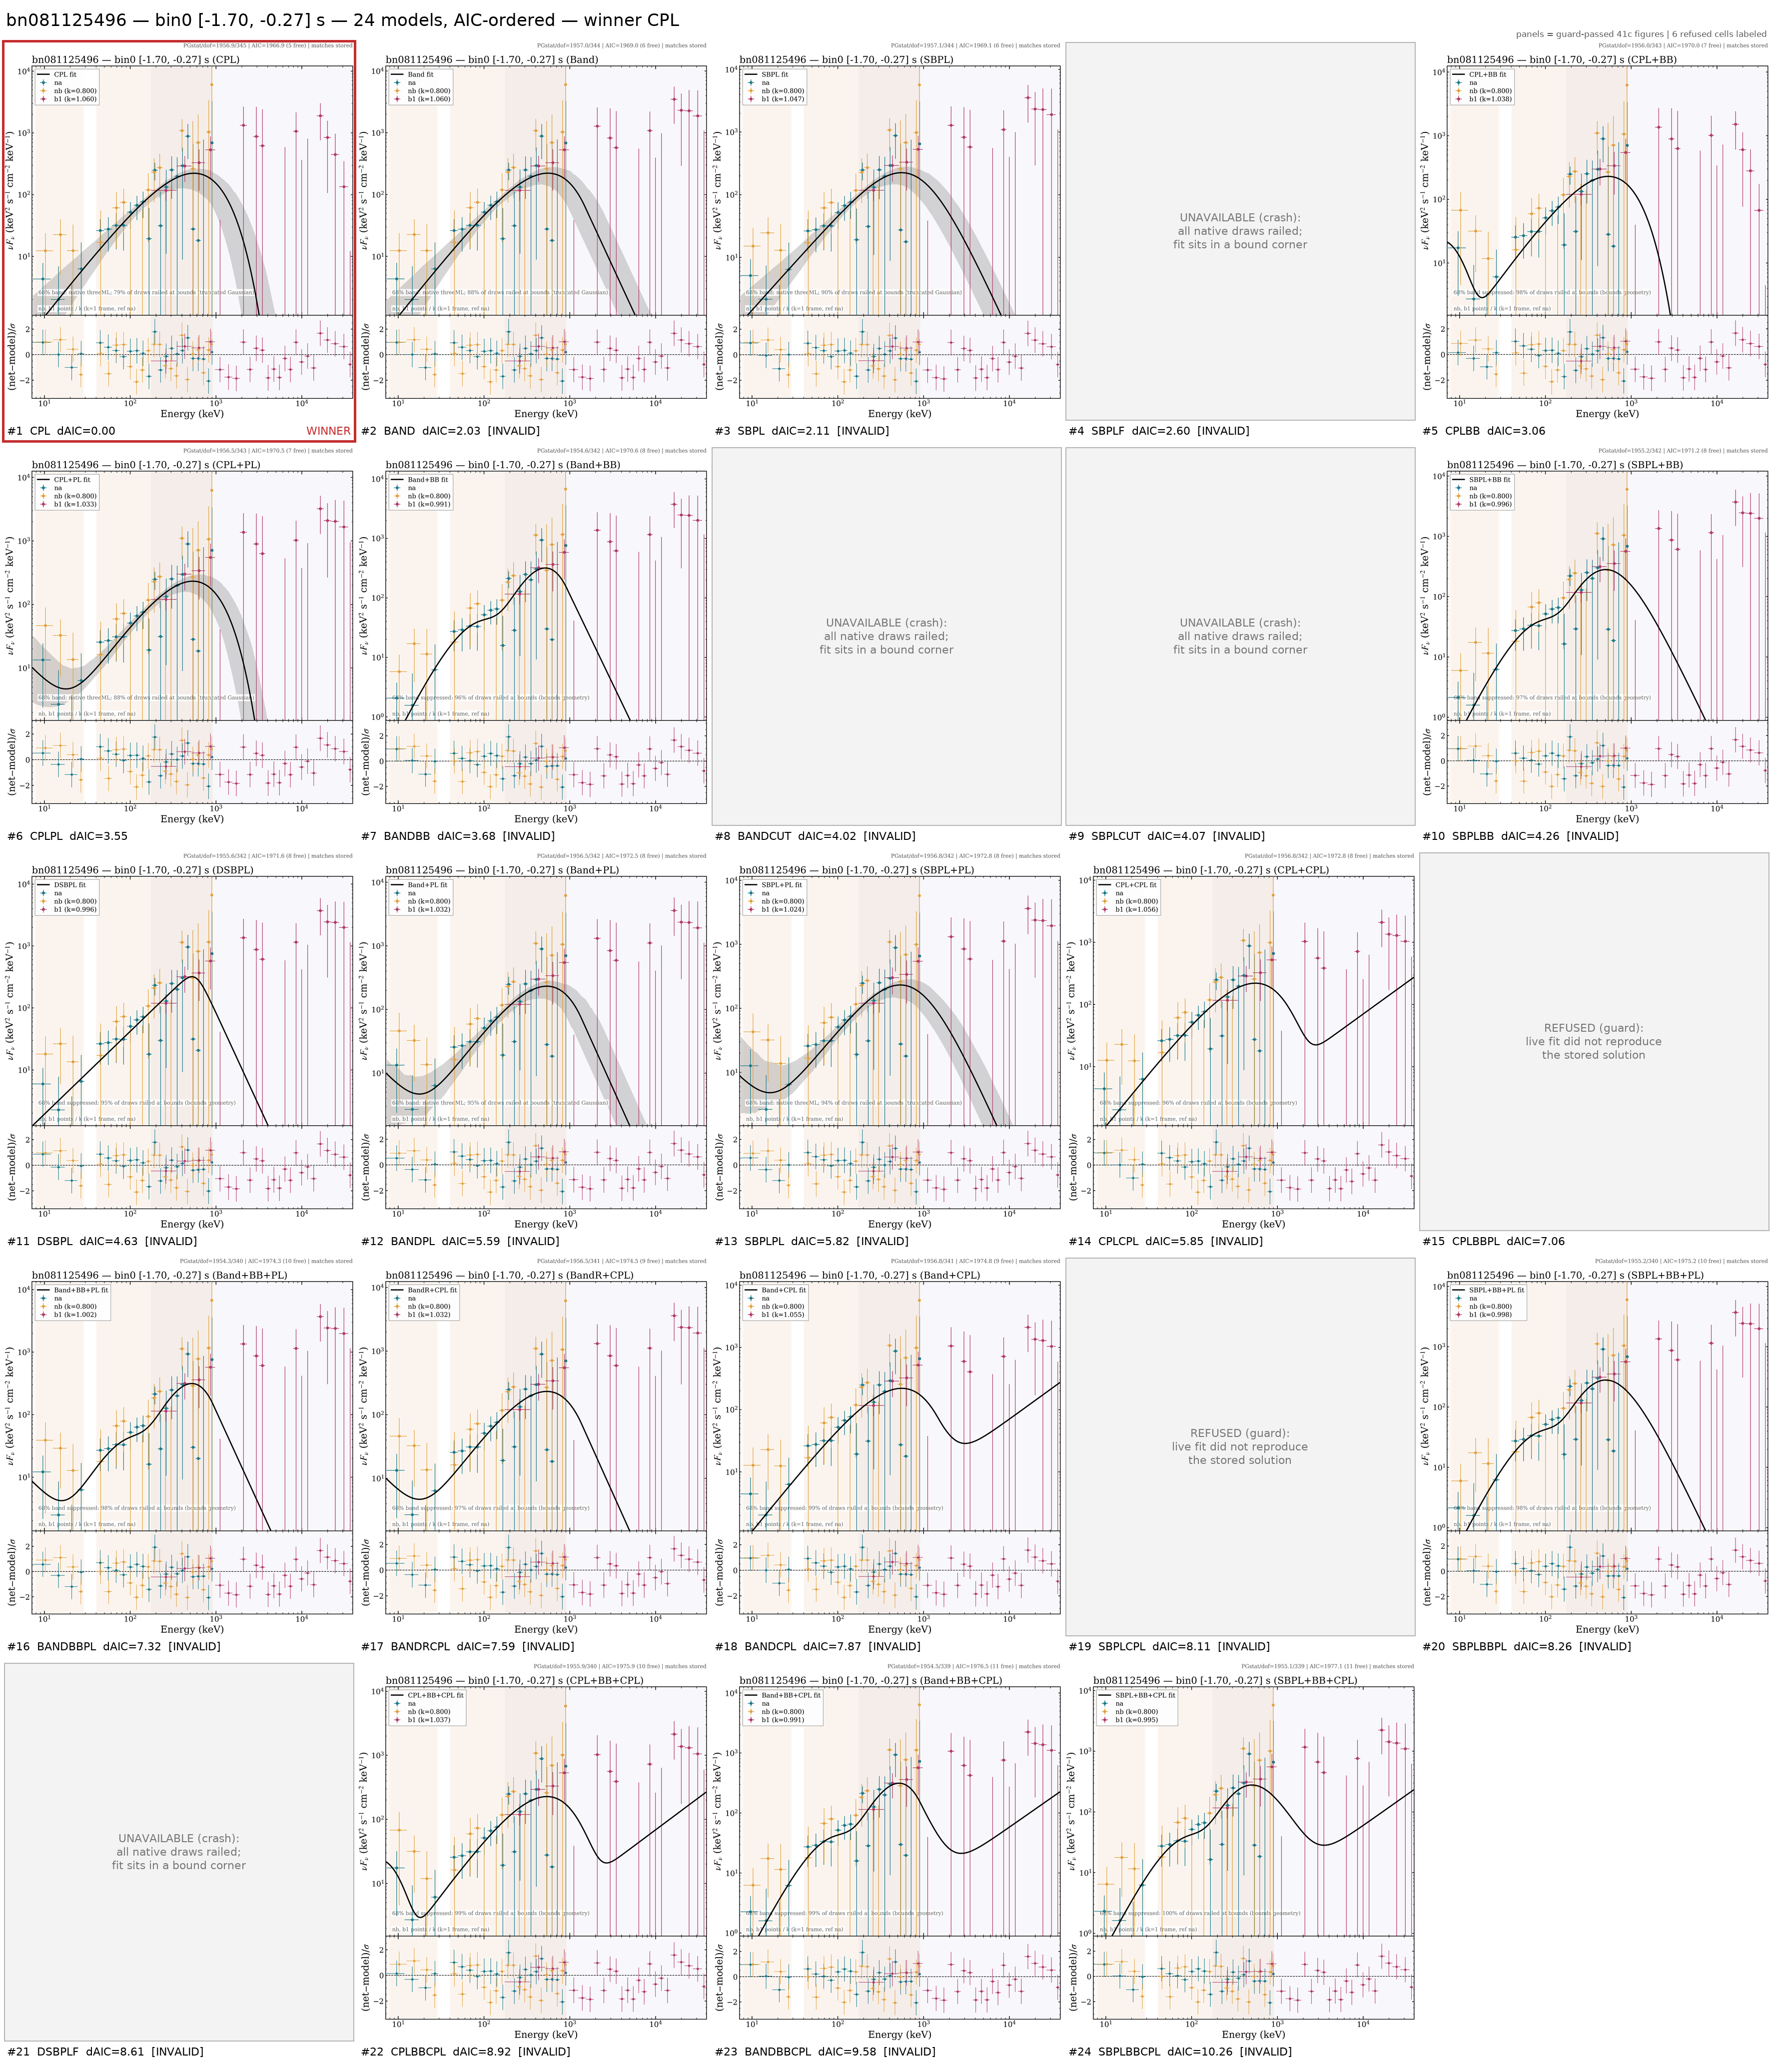
\includegraphics[width=\textwidth]{figs/bn081125496_montage_bin0.png}
\caption{Bin 0 montage.\label{fig:m0}}\end{figure*}
\begin{figure*}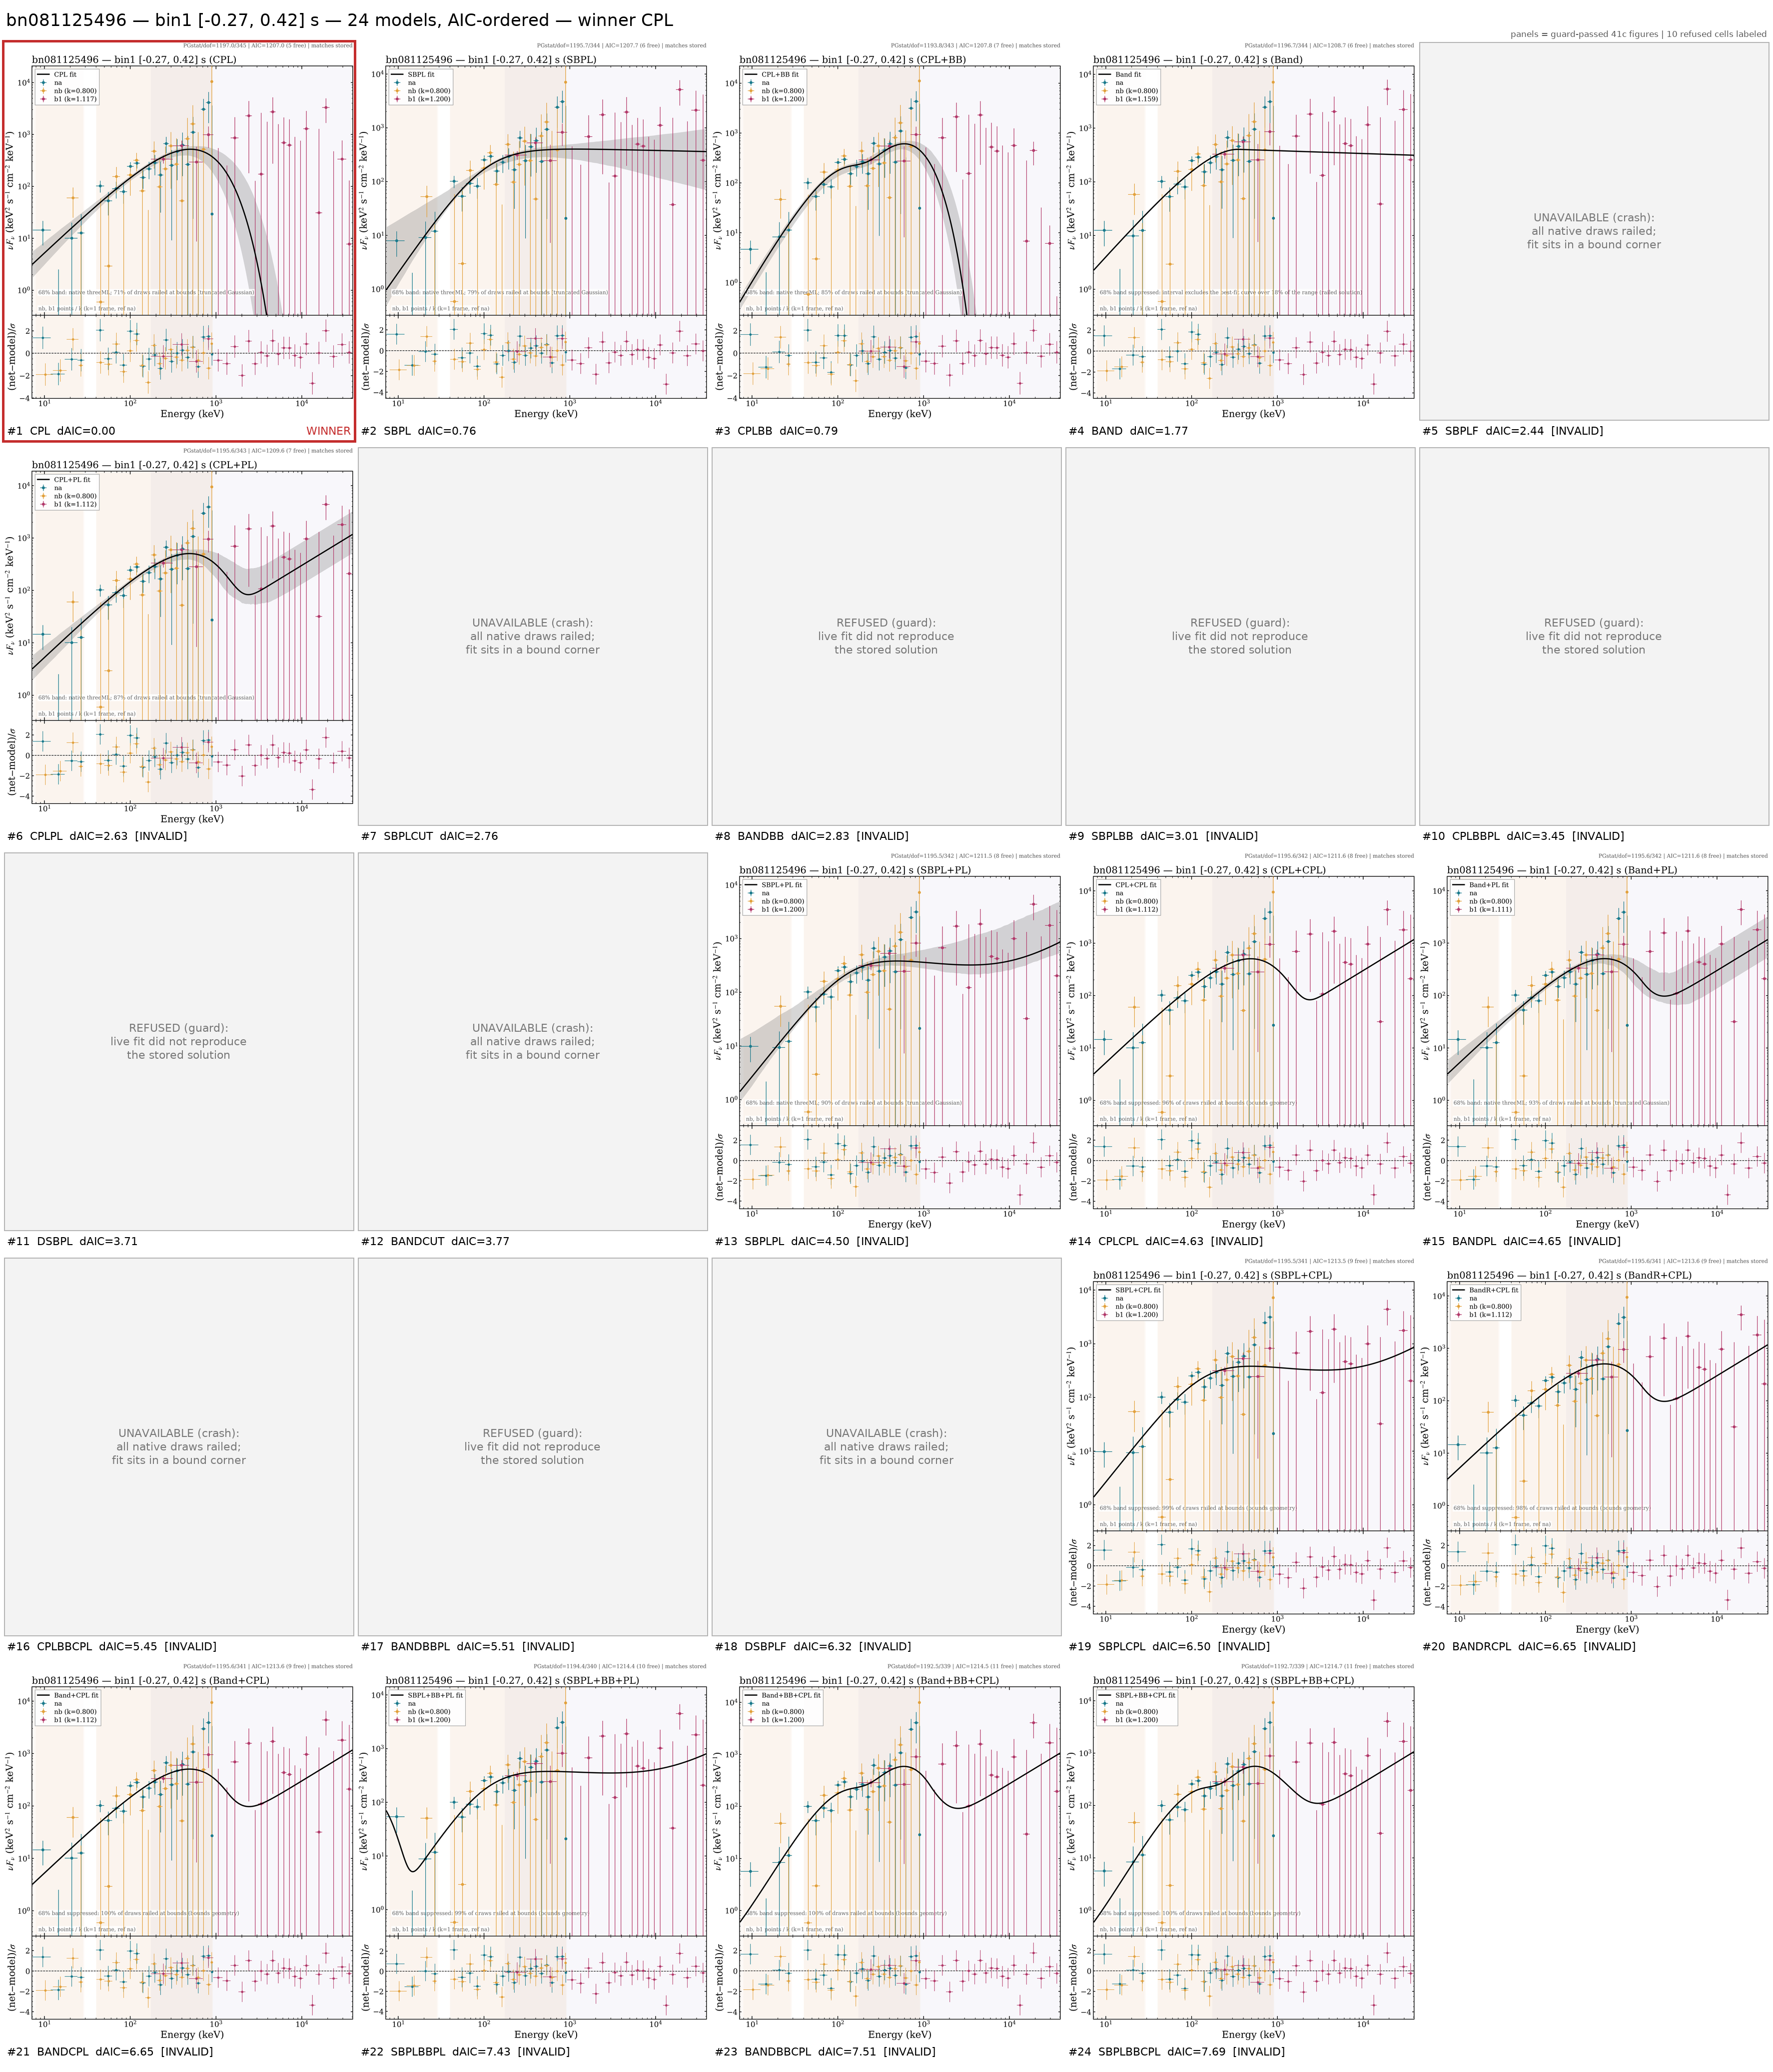
\includegraphics[width=\textwidth]{figs/bn081125496_montage_bin1.png}
\caption{Bin 1 montage.\label{fig:m1}}\end{figure*}
\begin{figure*}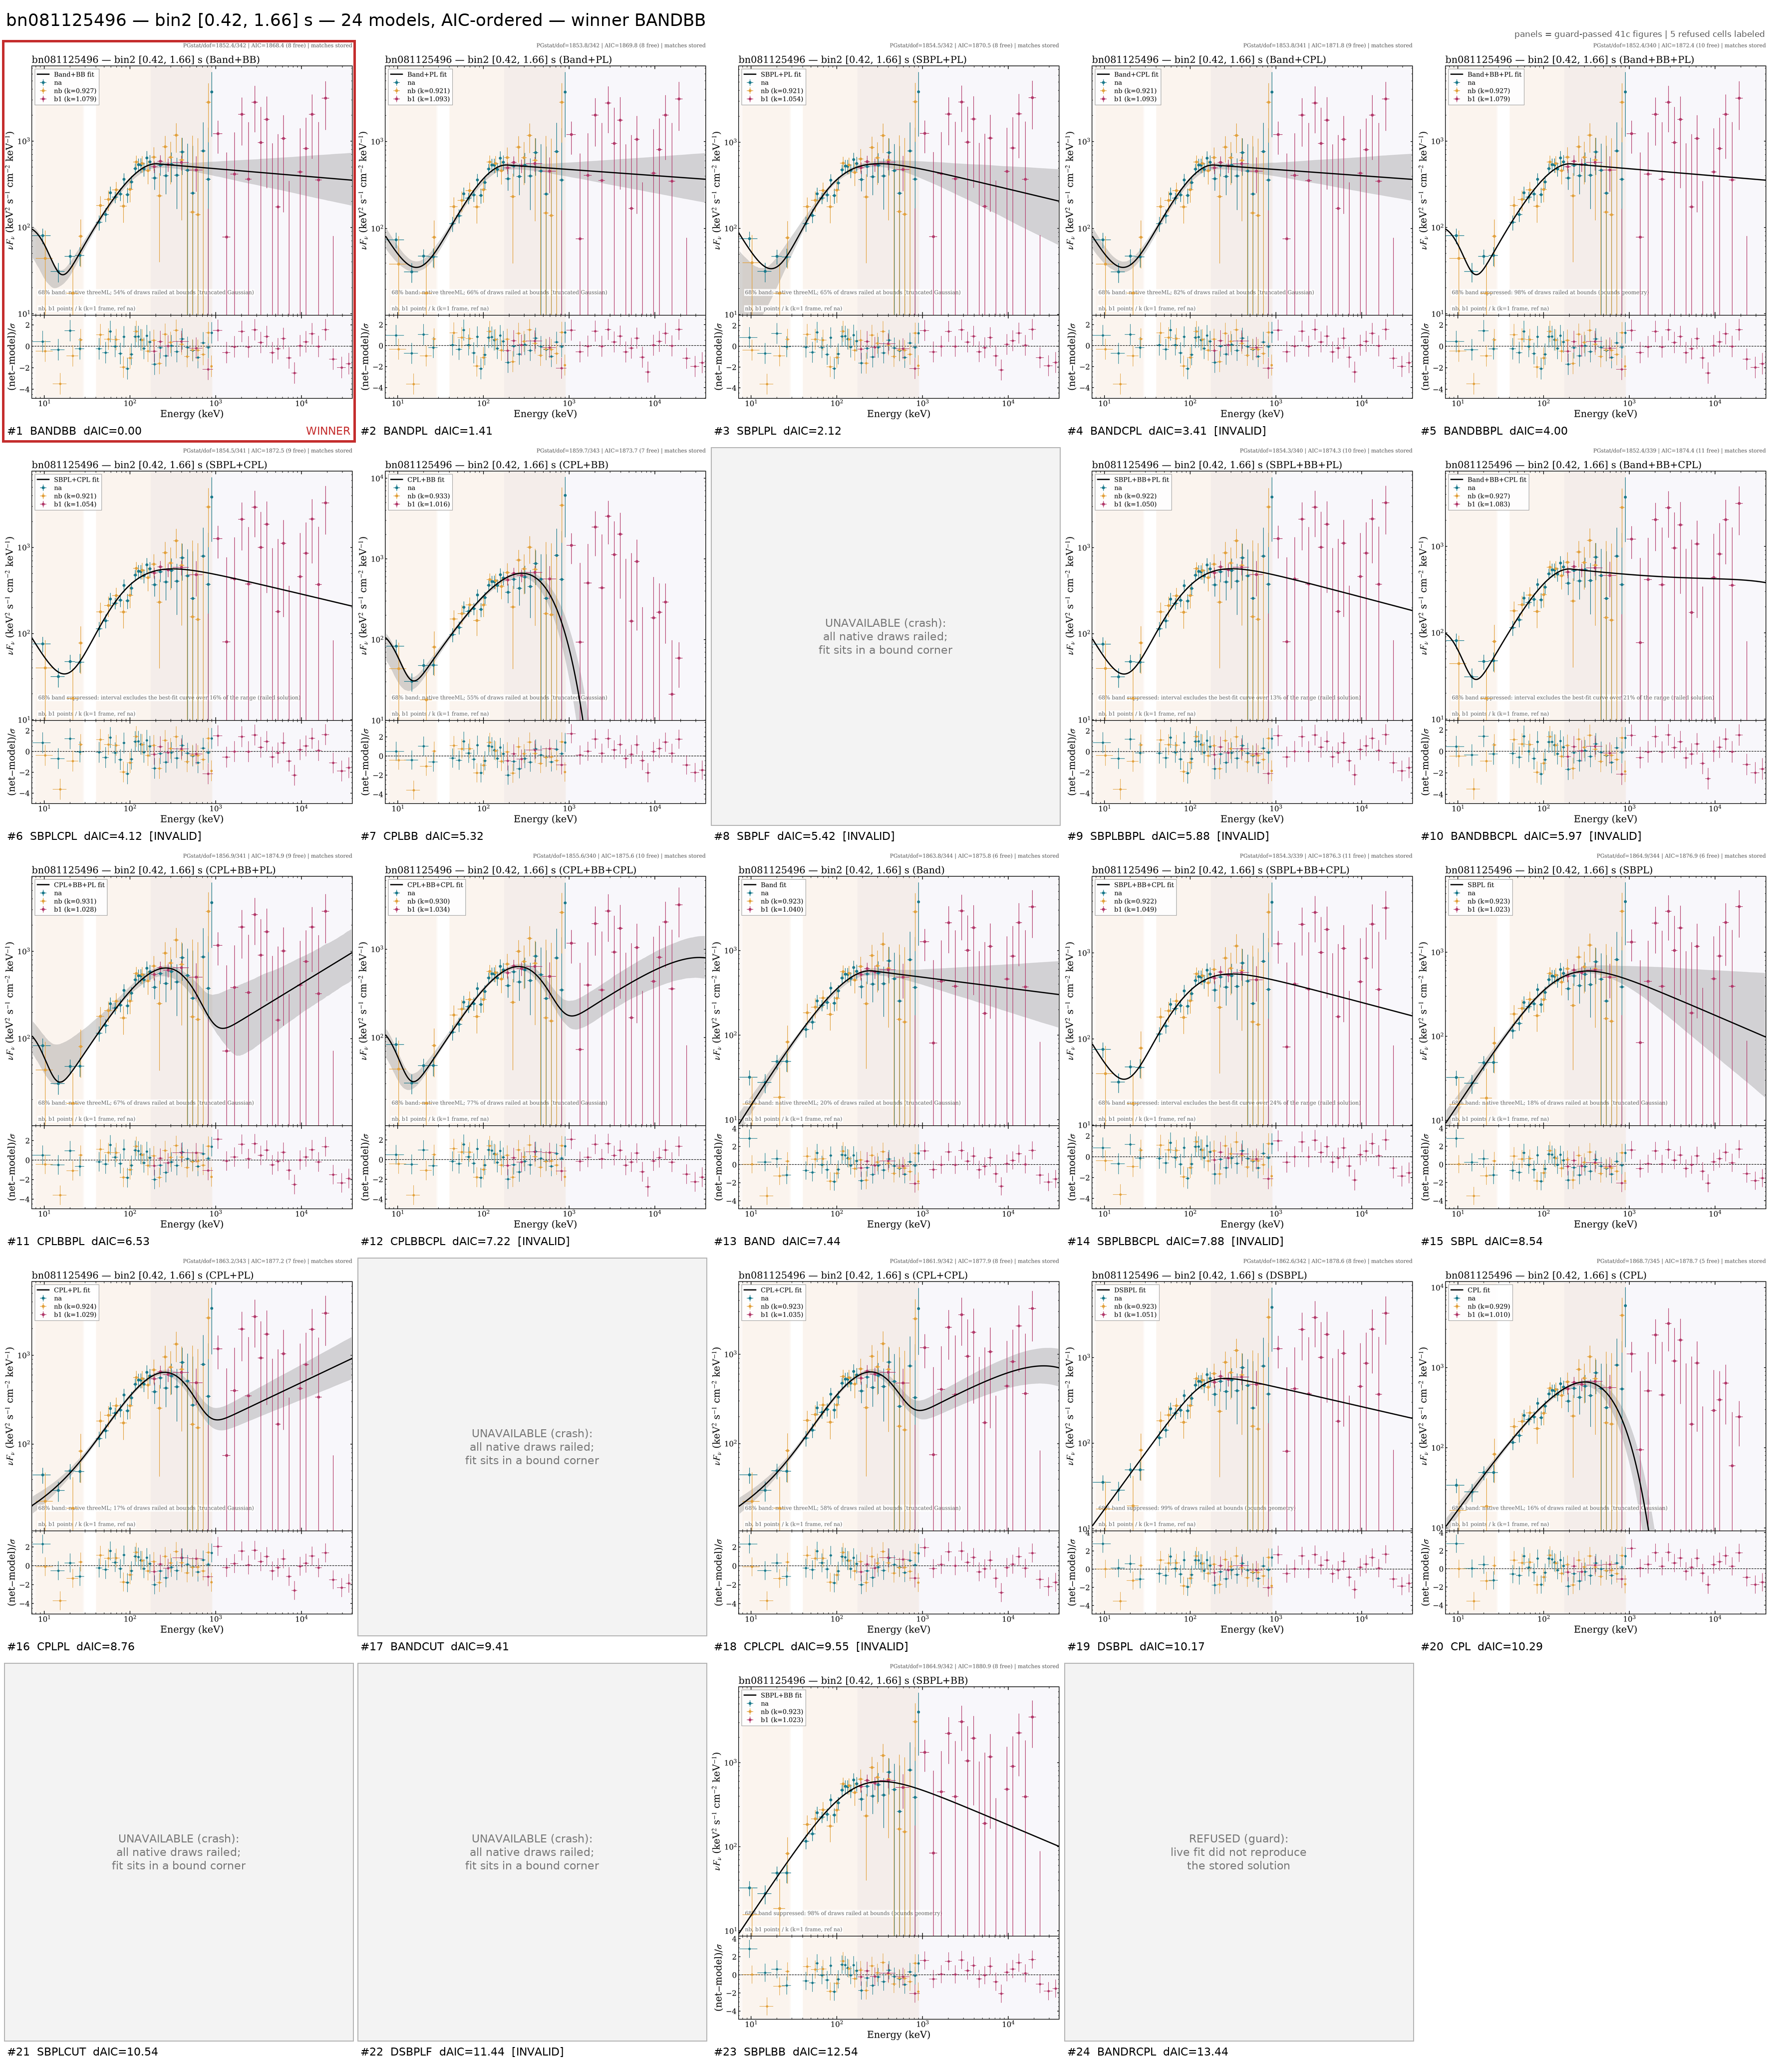
\includegraphics[width=\textwidth]{figs/bn081125496_montage_bin2.png}
\caption{Bin 2 montage.\label{fig:m2}}\end{figure*}
\begin{figure*}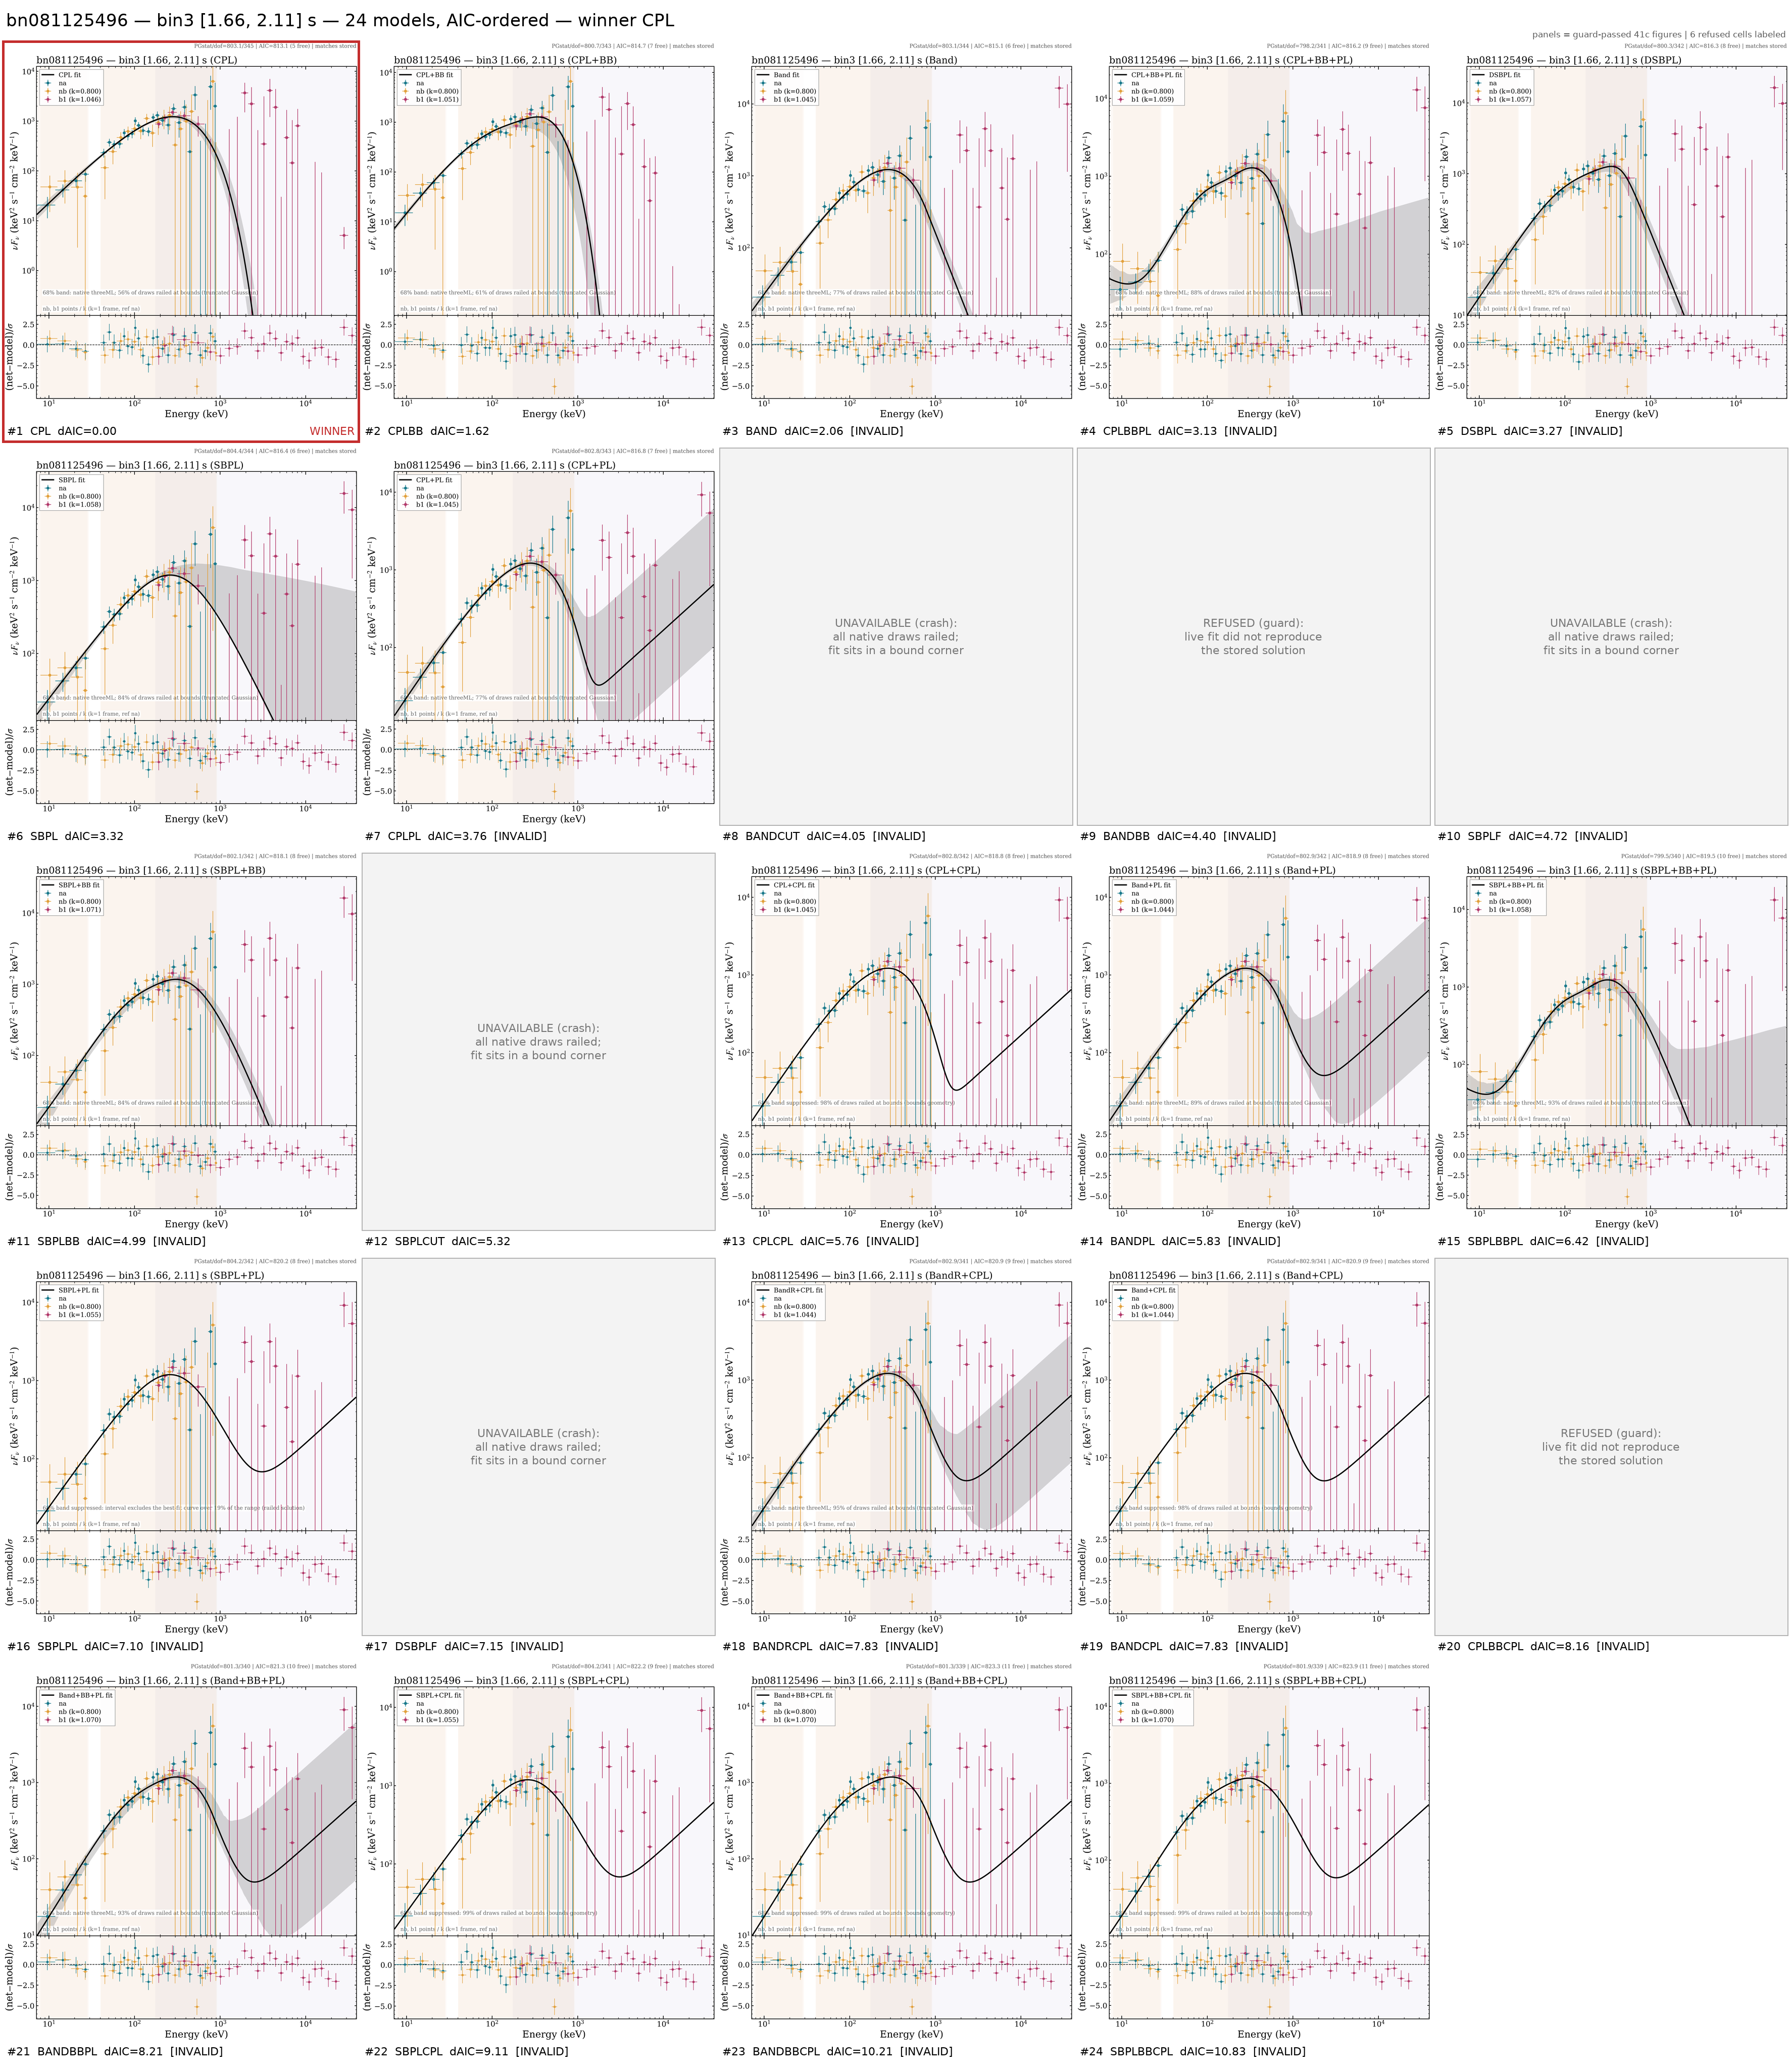
\includegraphics[width=\textwidth]{figs/bn081125496_montage_bin3.png}
\caption{Bin 3 montage.\label{fig:m3}}\end{figure*}
\begin{figure*}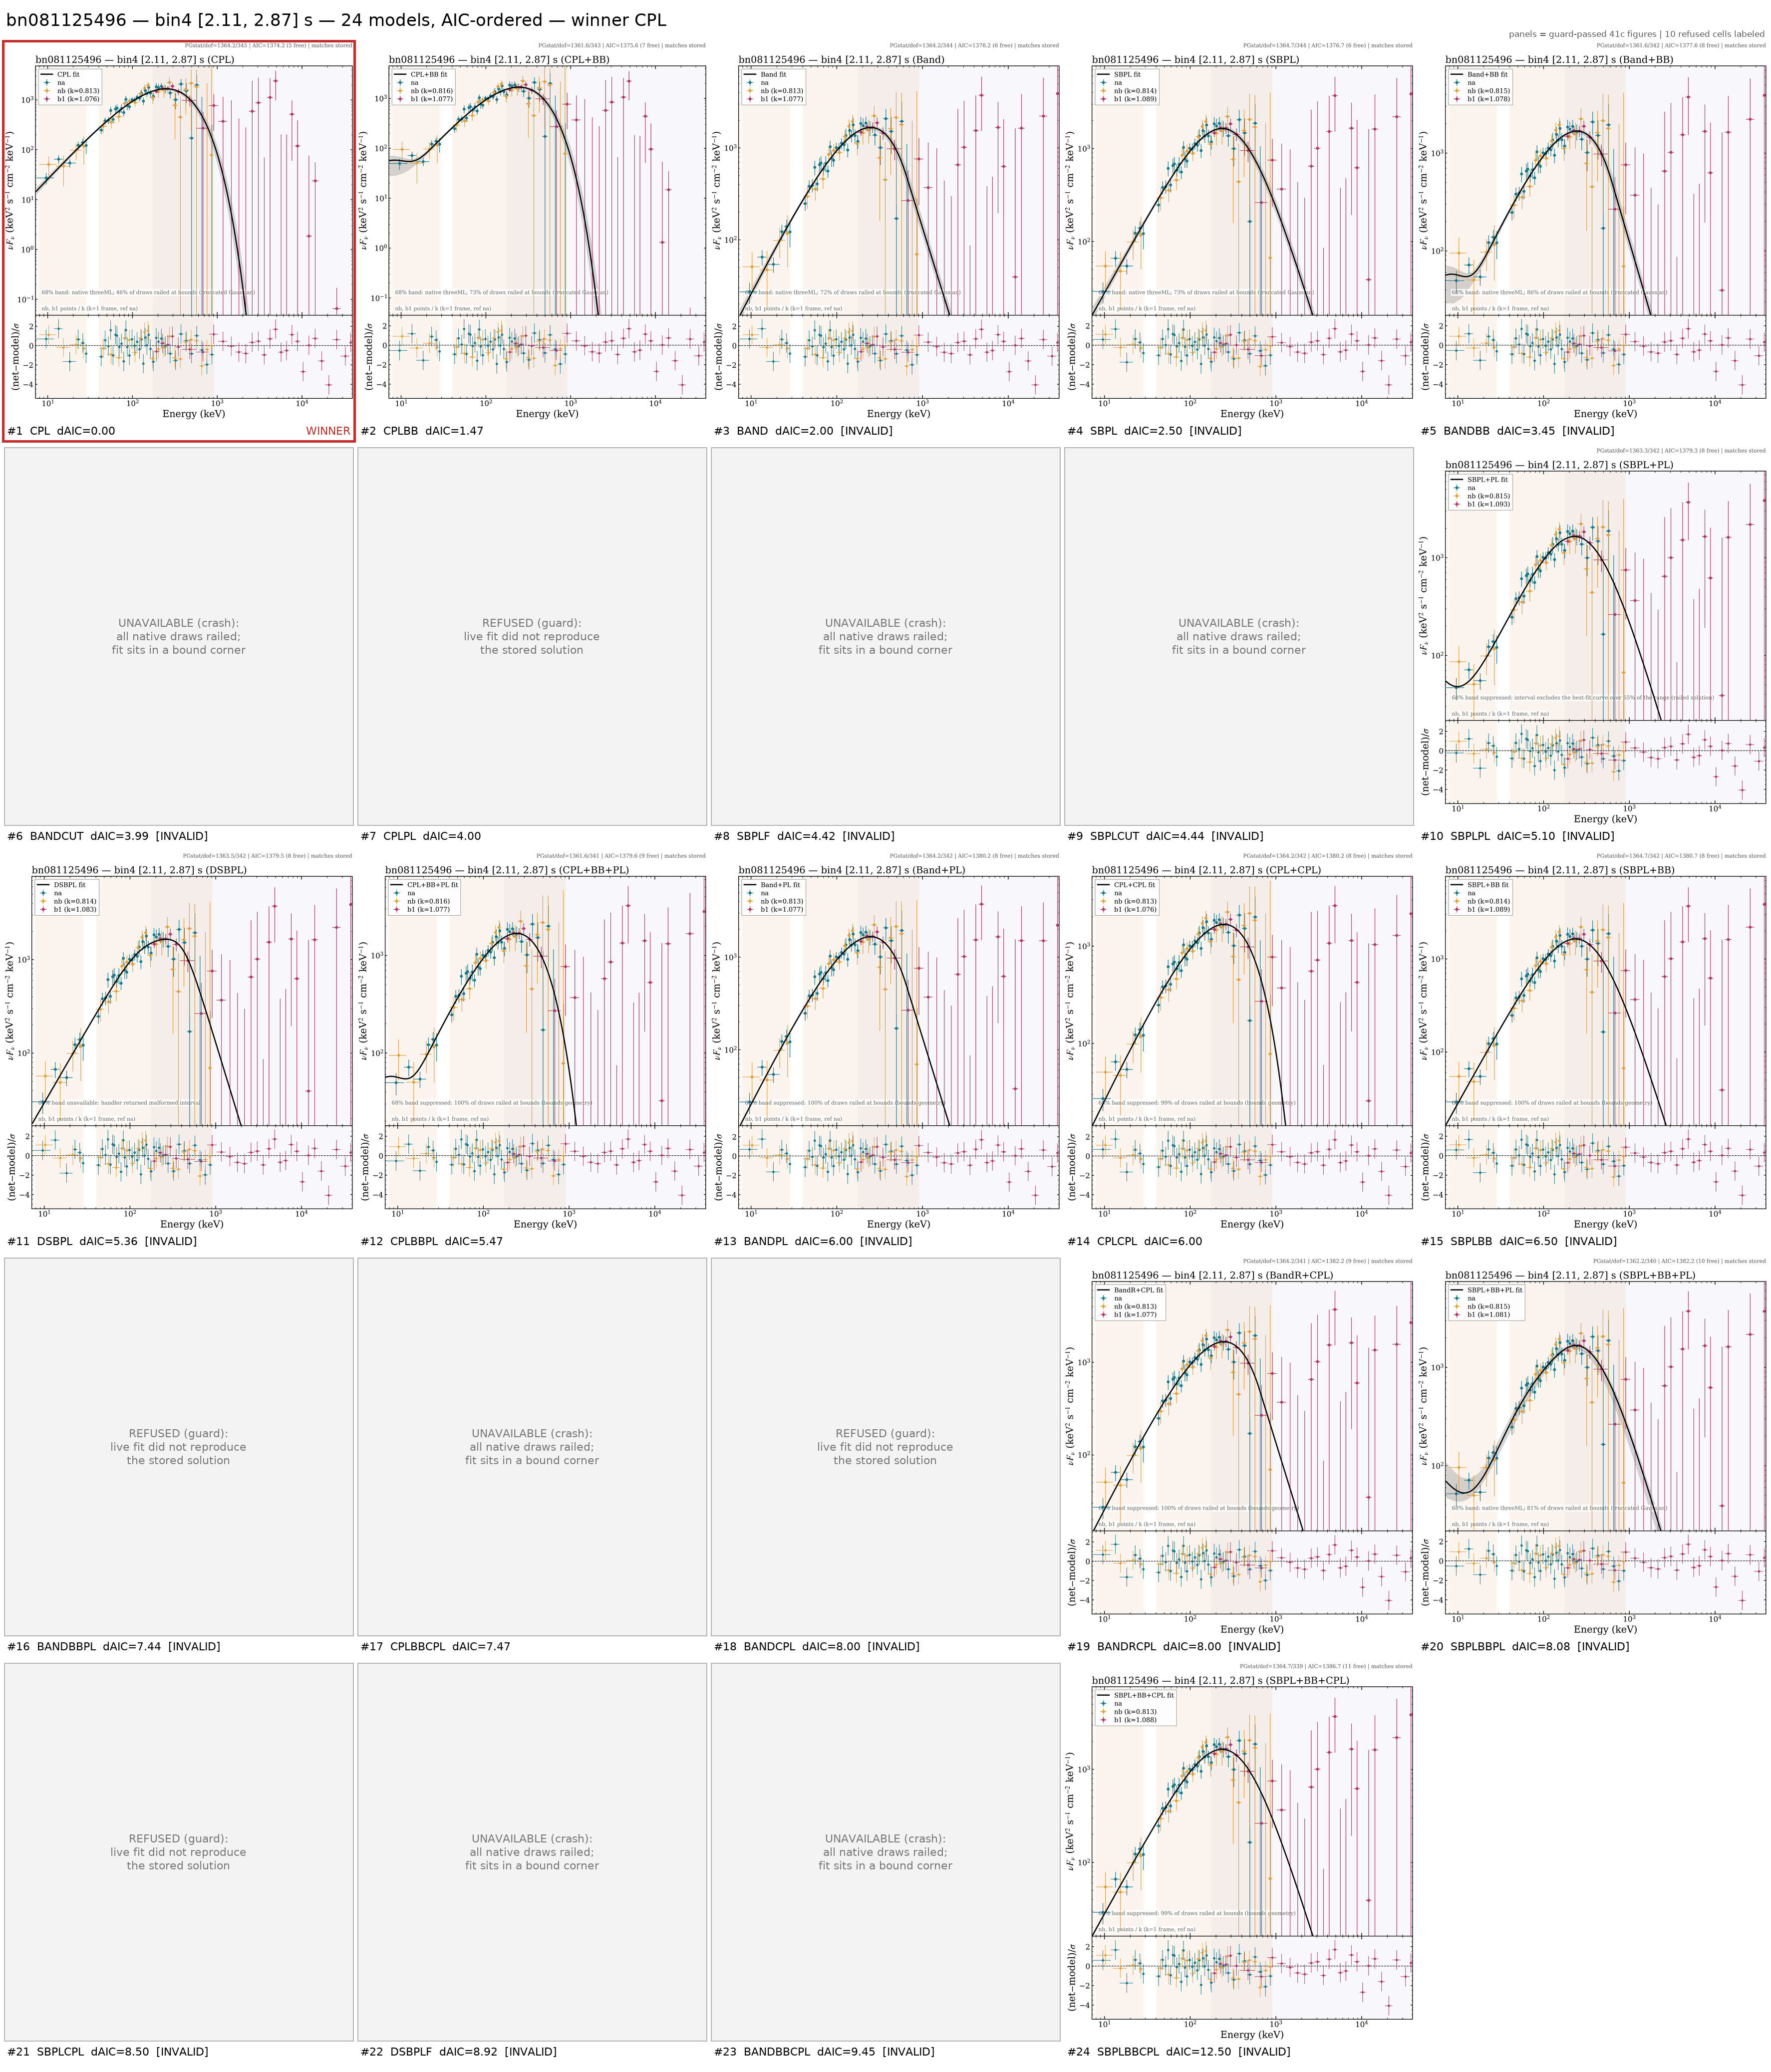
\includegraphics[width=\textwidth]{figs/bn081125496_montage_bin4.png}
\caption{Bin 4 montage.\label{fig:m4}}\end{figure*}
\begin{figure*}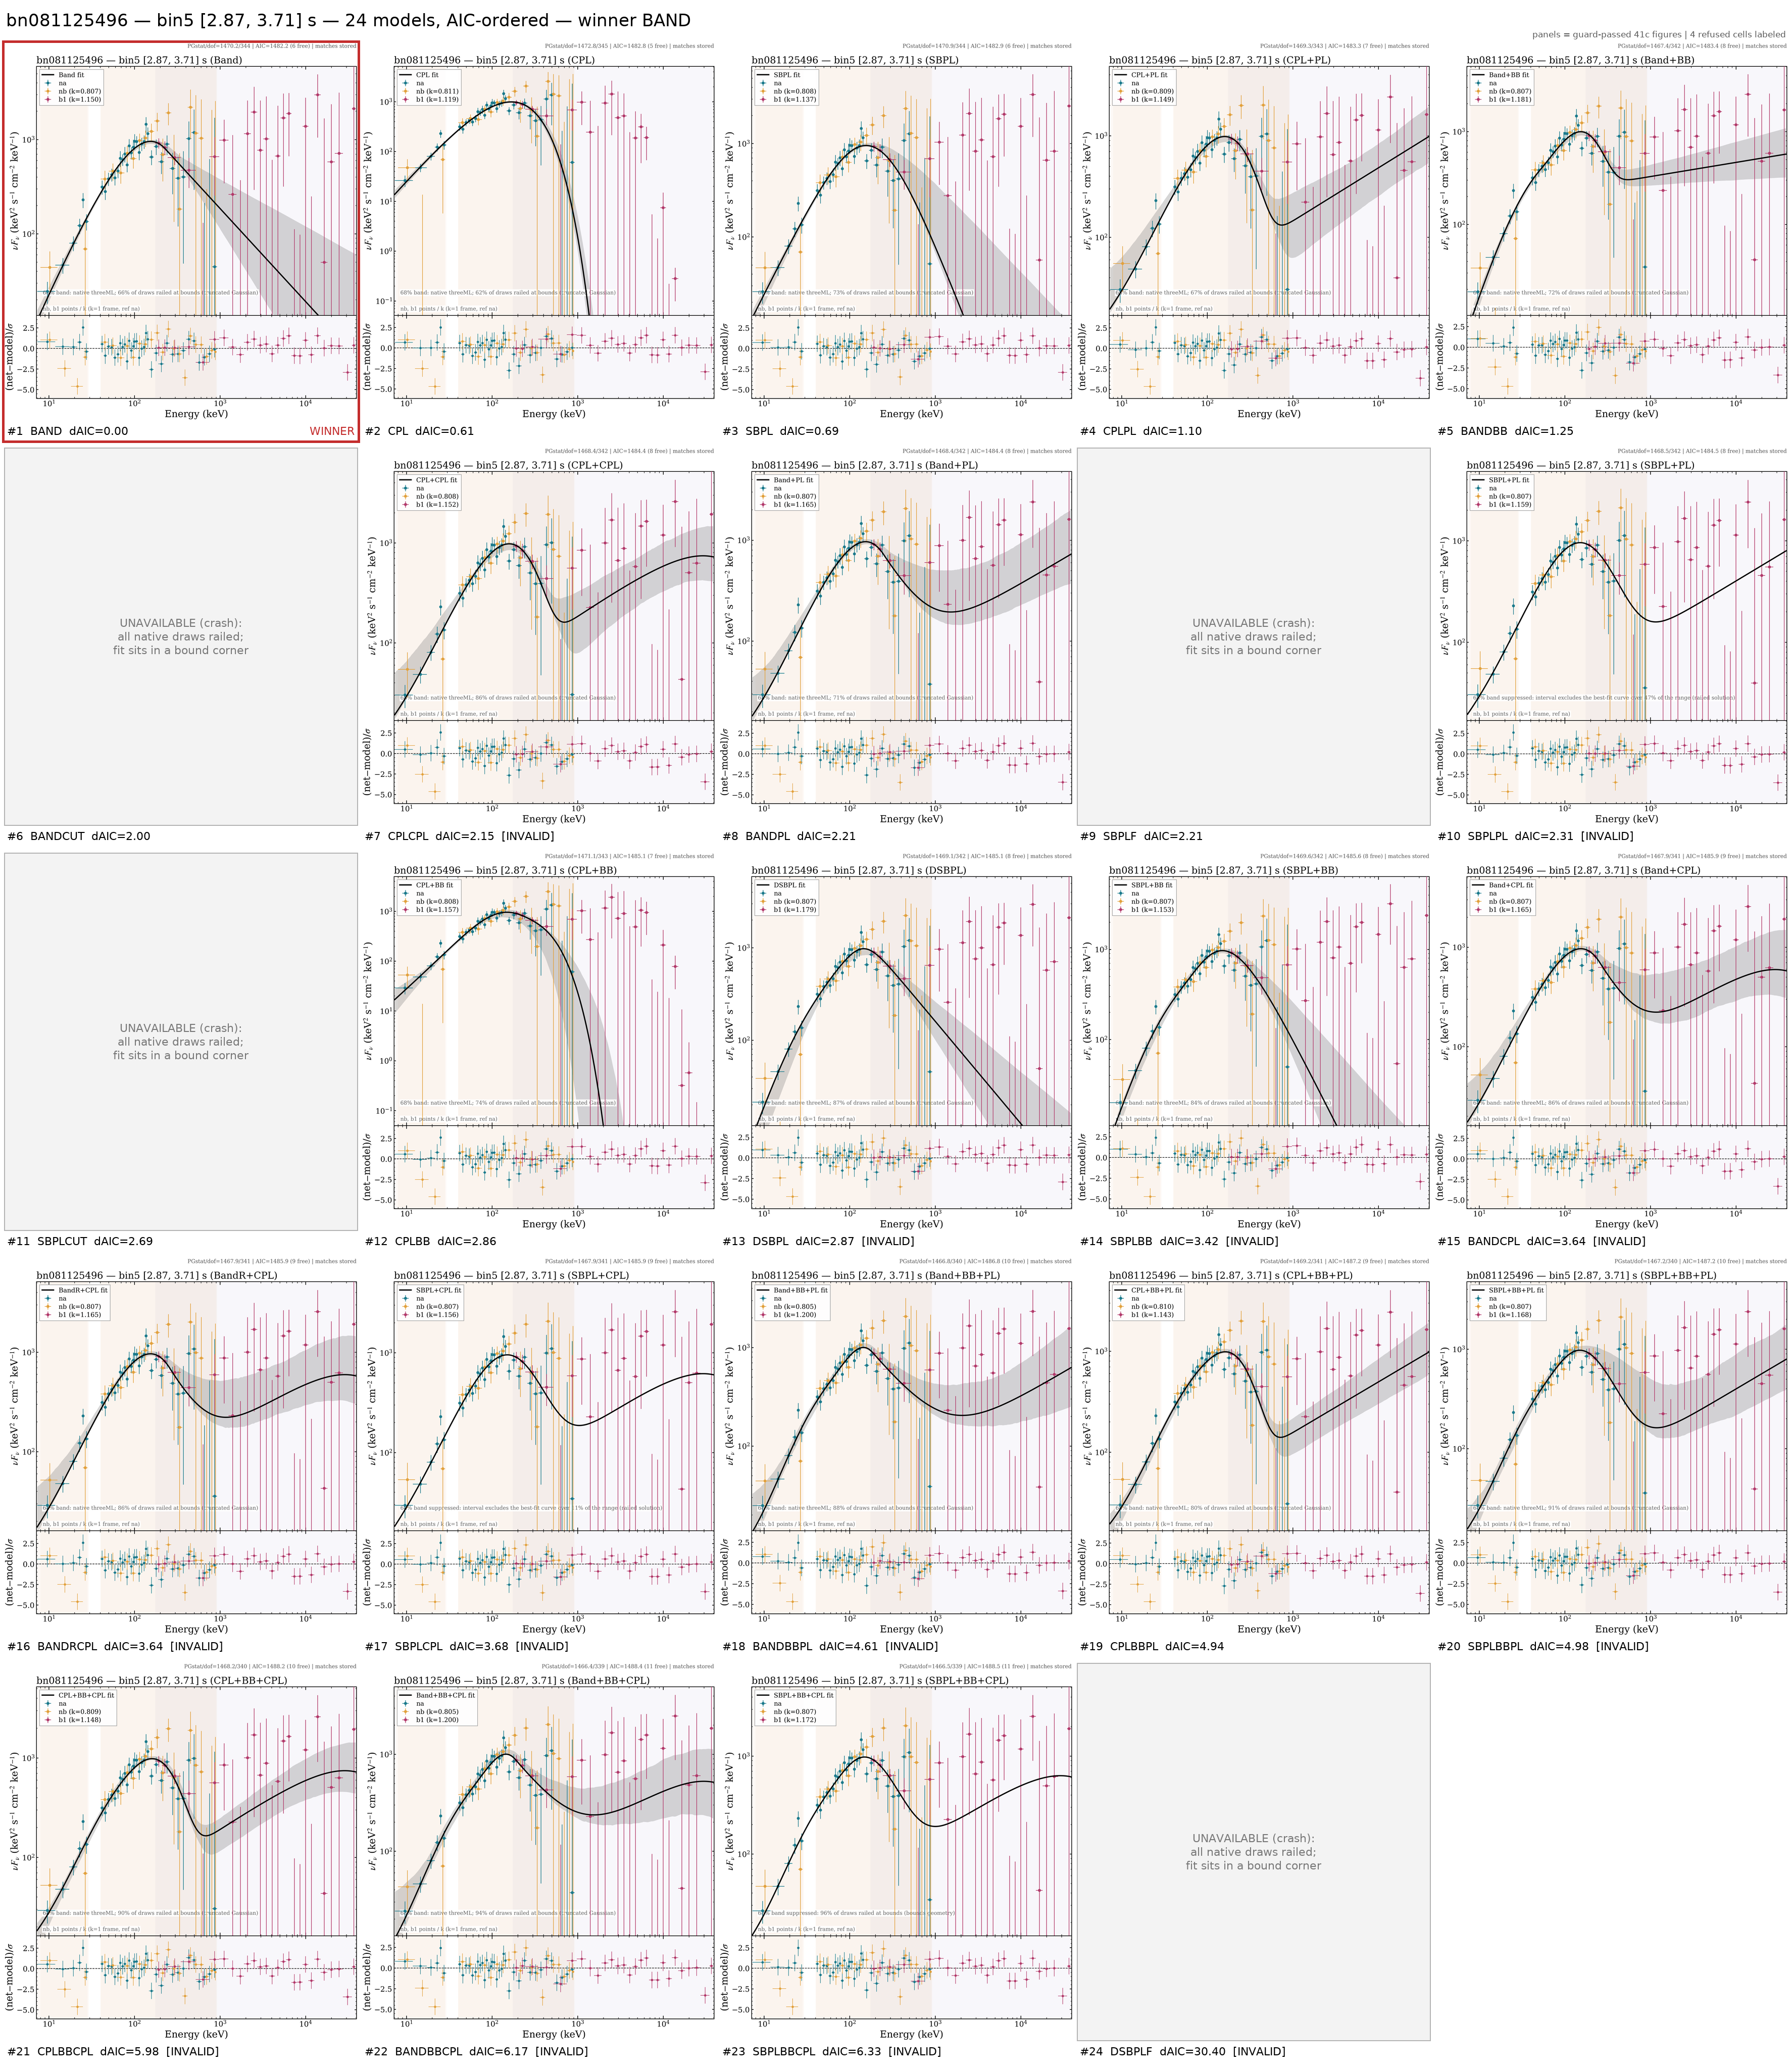
\includegraphics[width=\textwidth]{figs/bn081125496_montage_bin5.png}
\caption{Bin 5 montage.\label{fig:m5}}\end{figure*}
\begin{figure*}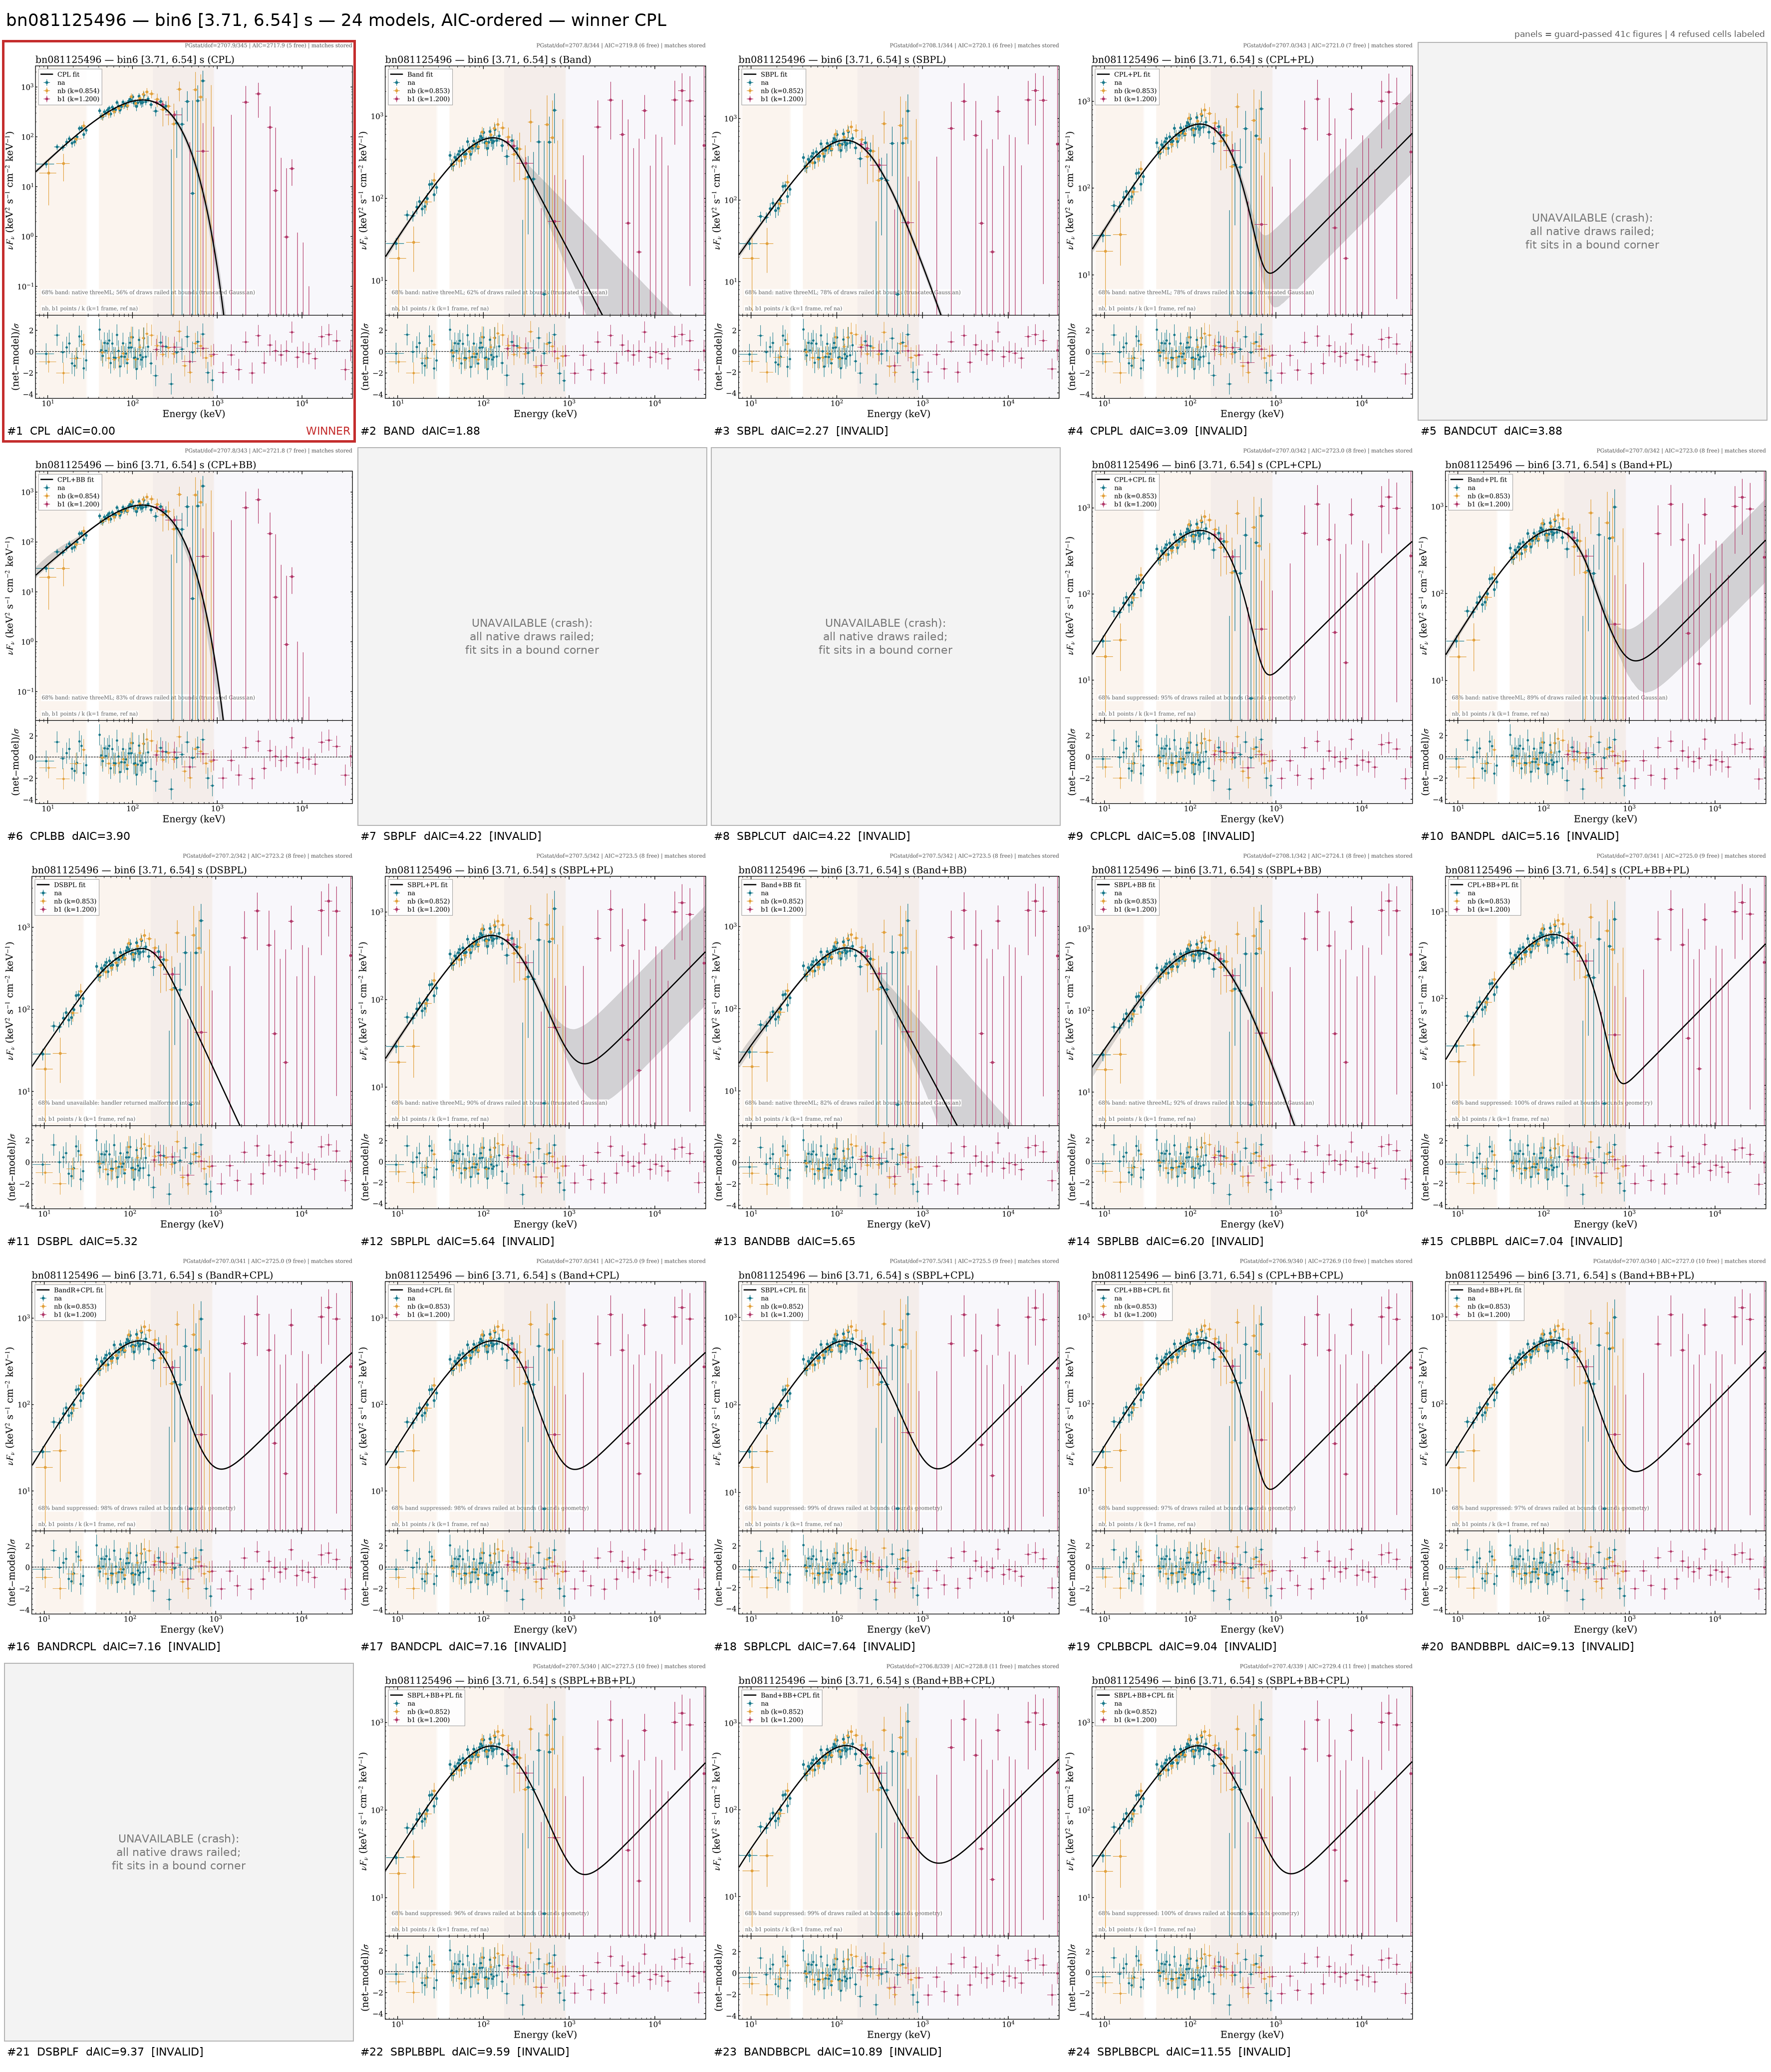
\includegraphics[width=\textwidth]{figs/bn081125496_montage_bin6.png}
\caption{Bin 6 montage.\label{fig:m6}}\end{figure*}
\begin{figure*}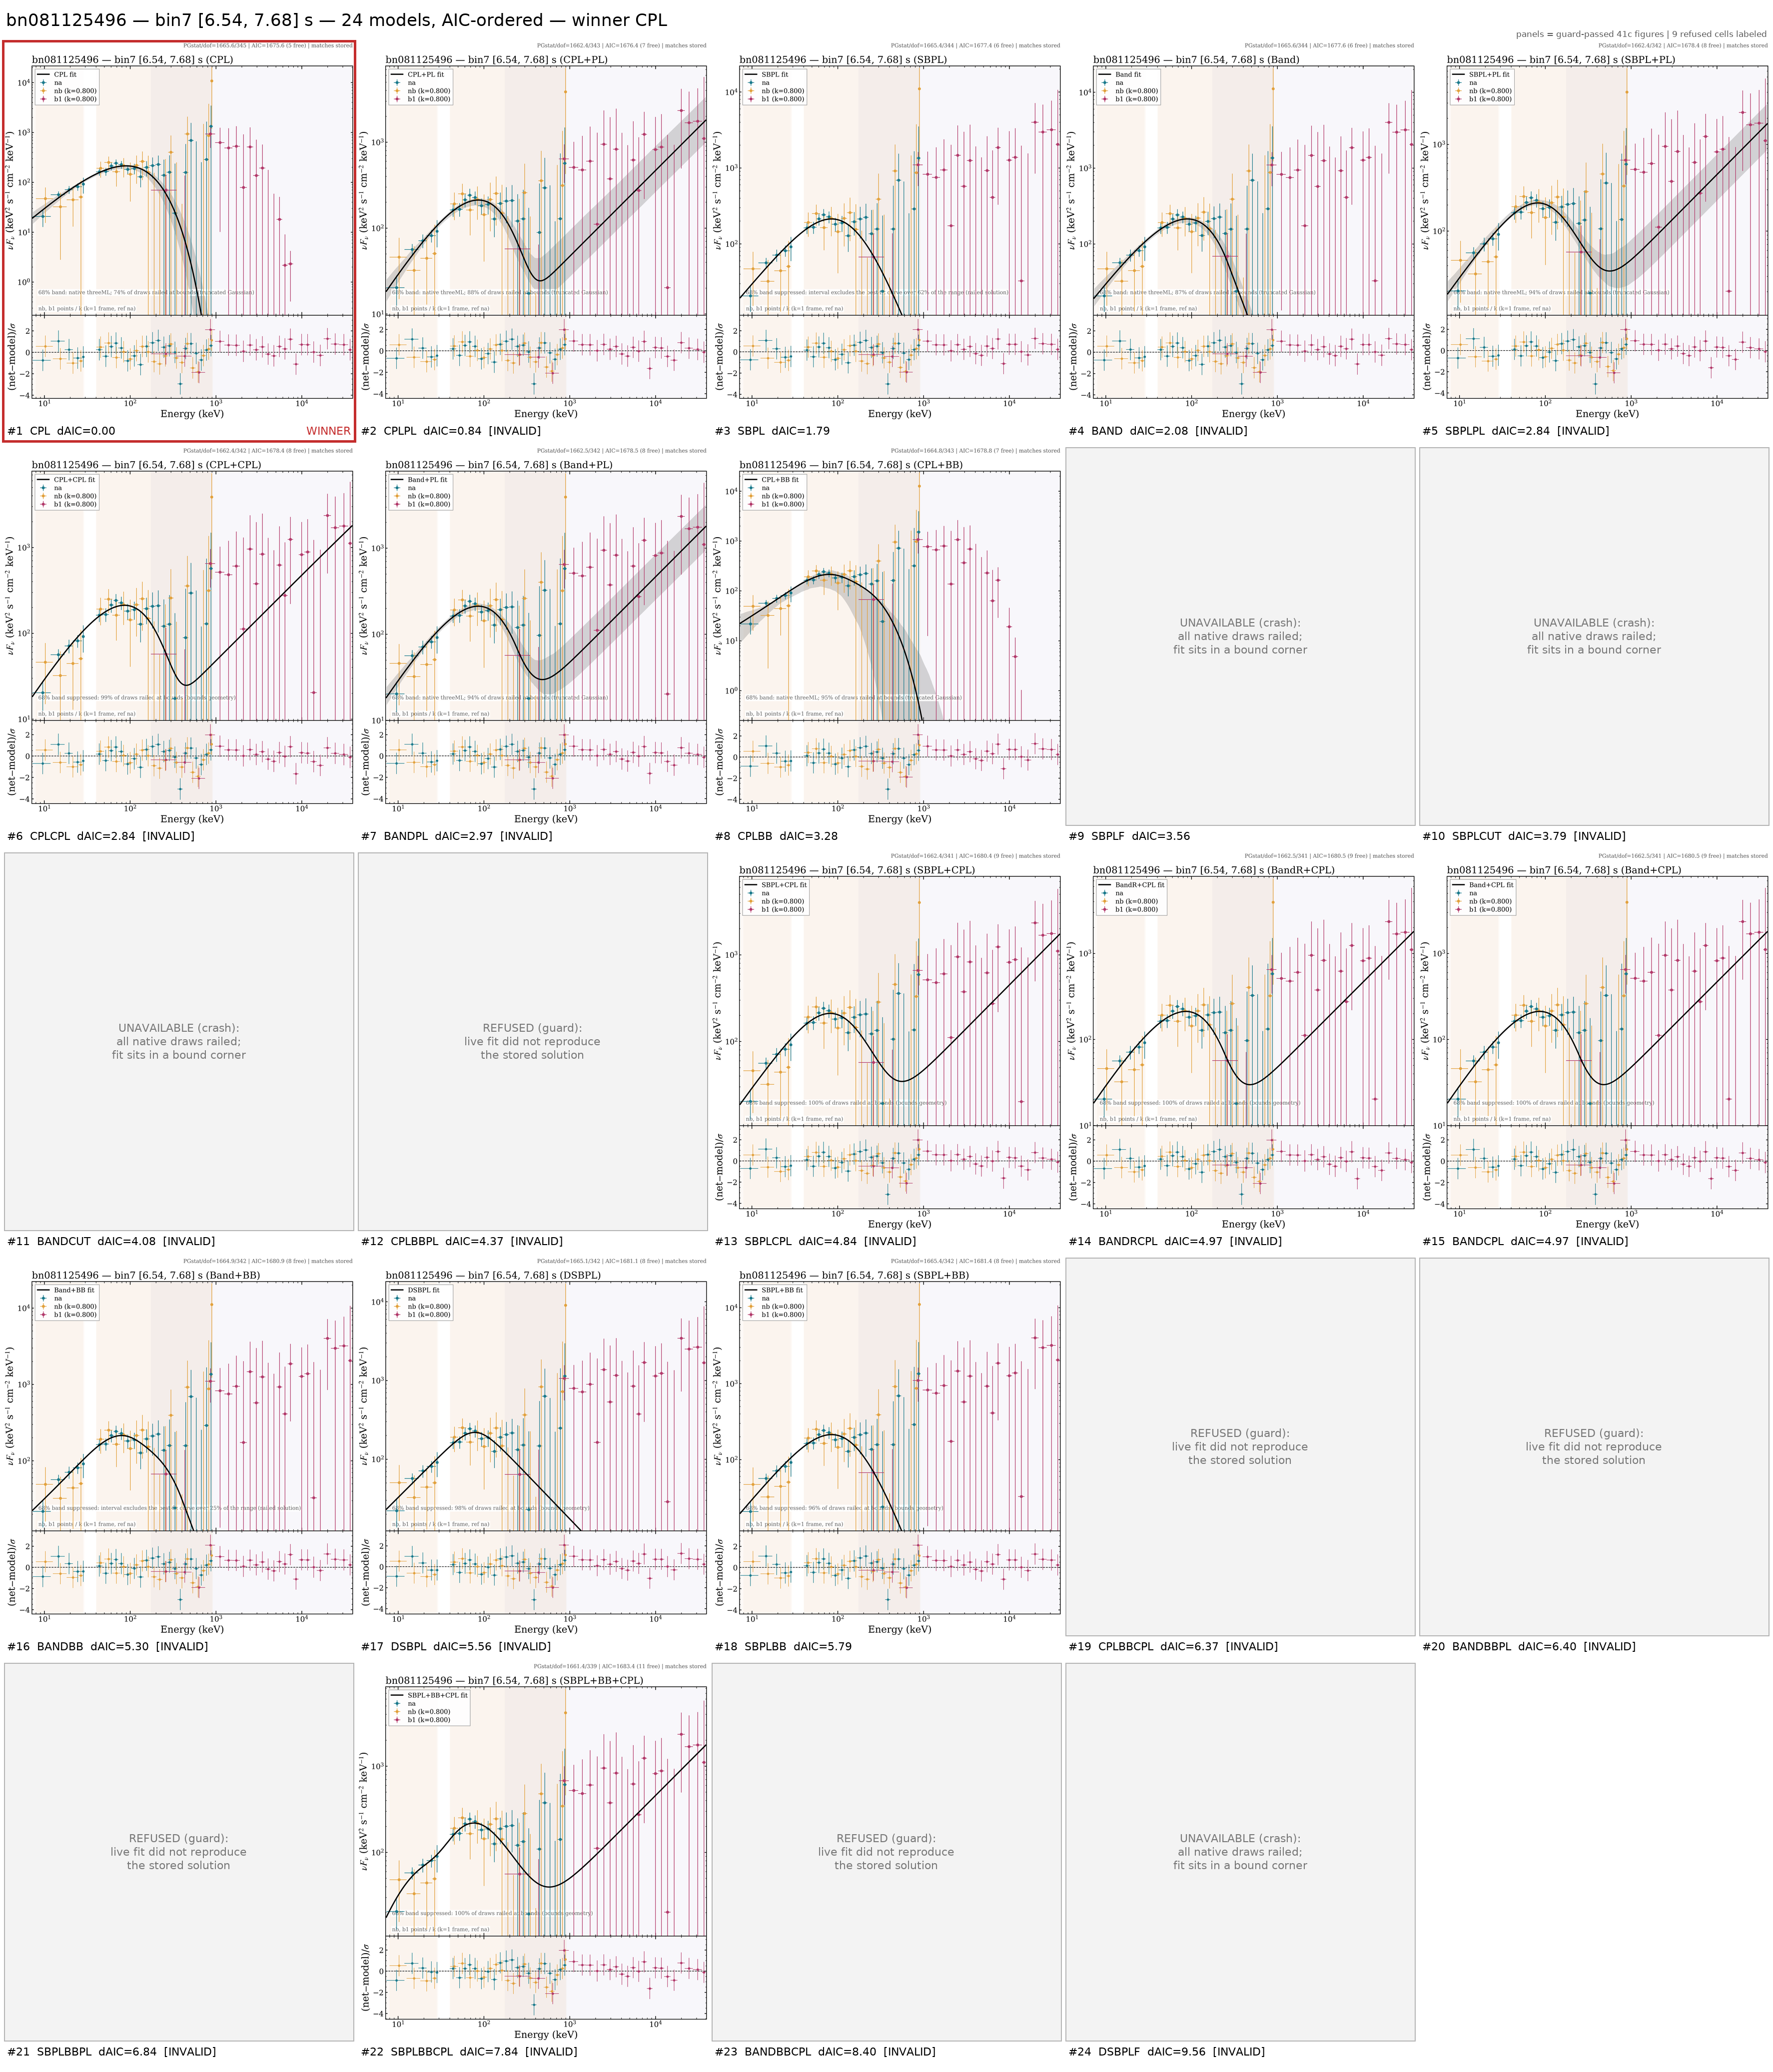
\includegraphics[width=\textwidth]{figs/bn081125496_montage_bin7.png}
\caption{Bin 7 montage.\label{fig:m7}}\end{figure*}
\begin{figure*}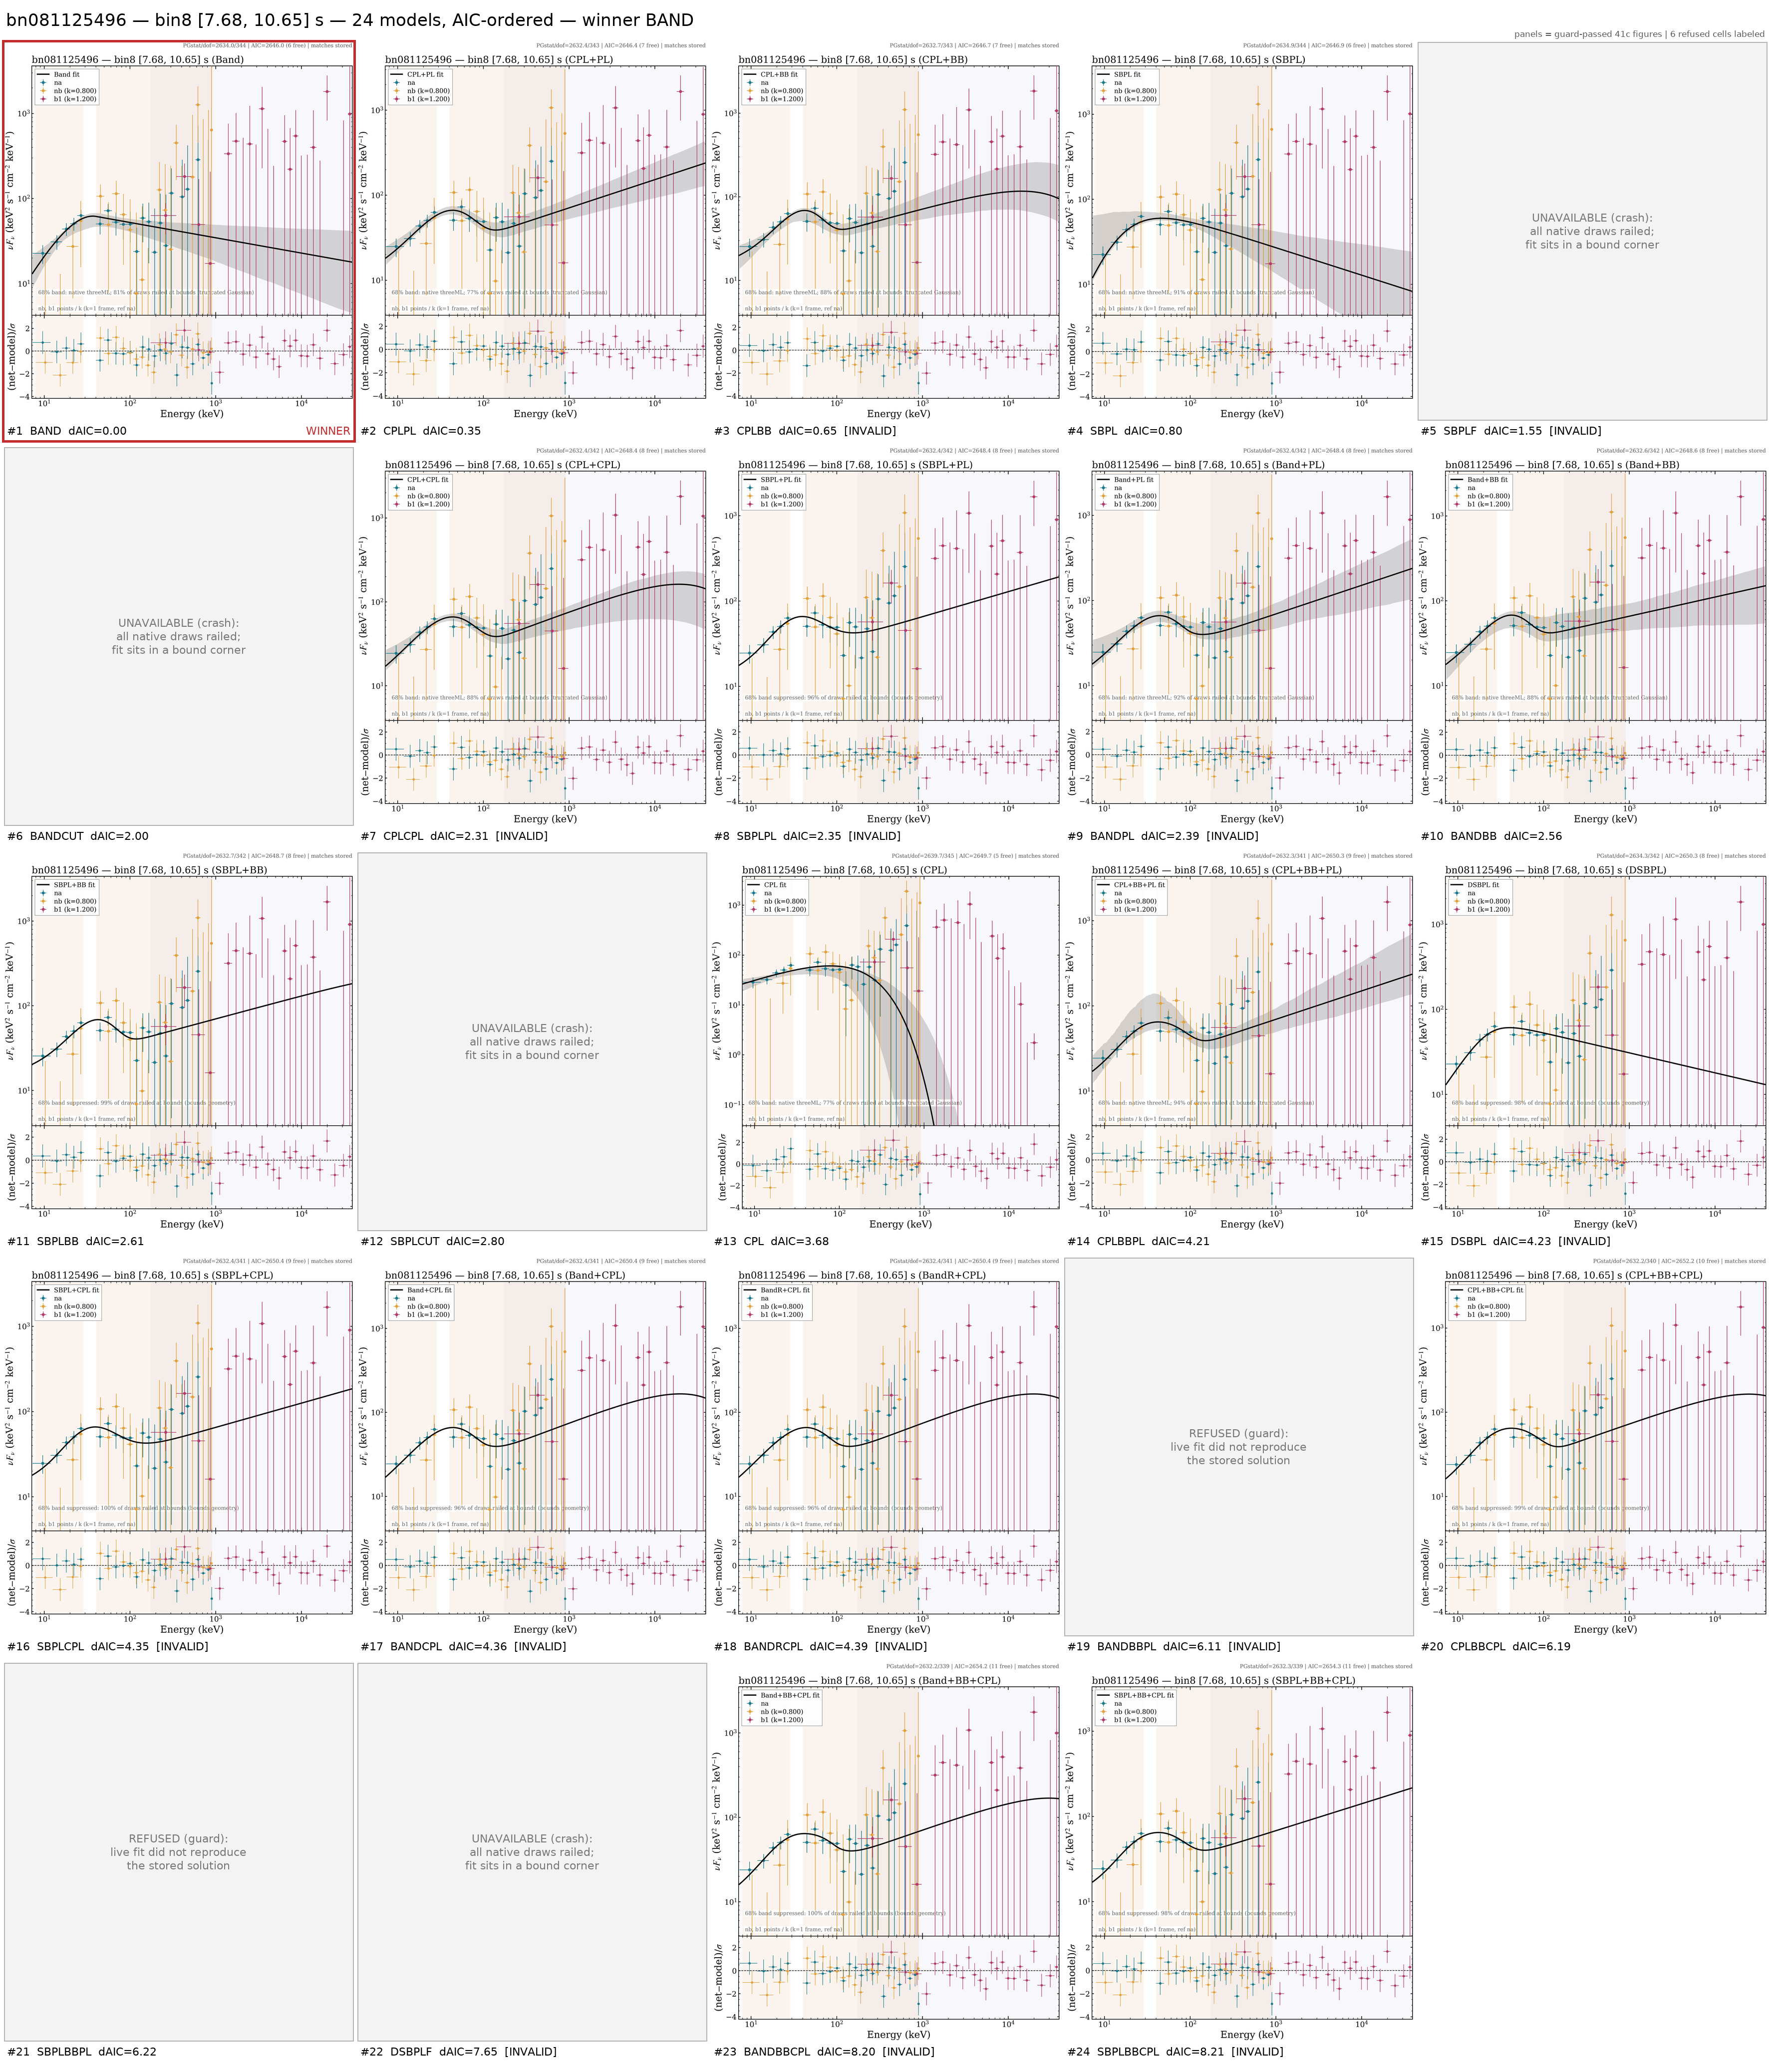
\includegraphics[width=\textwidth]{figs/bn081125496_montage_bin8.png}
\caption{Bin 8 montage.\label{fig:m8}}\end{figure*}

\bibliography{refs}
\bibliographystyle{aasjournal}

\end{document}
